\documentclass[degree=master]{thuthesis}
% 选项:
%   degree=[bachelor|master|doctor|postdoctor], % 必选
%   secret,                                     % 可选
%   pifootnote,                                 % 可选(建议打开)
%   openany|openright,                          % 可选,基本不用
%   arial,                                      % 可选,基本不用
%   arialtoc,                                   % 可选,基本不用
%   arialtitle                                  % 可选,基本不用

% 所有其它可能用到的包都统一放到这里了,可以根据自己的实际添加或者删除。
\usepackage{thuthesis}

% 定义所有的图片文件在 figures 子目录下
\graphicspath{{figures/}}

% 可以在这里修改配置文件中的定义。导言区可以使用中文。
% \def\myname{薛瑞尼}

\begin{document}

%%% 封面部分
\frontmatter
\thusetup{
  %******************************
  % 注意:
  %   1. 配置里面不要出现空行
  %   2. 不需要的配置信息可以删除
  %******************************
  %
  %=====
  % 秘级
  %=====
  secretlevel={秘密},
  secretyear={10},
  %
  %=========
  % 中文信息
  %=========
  ctitle={清华大学学位论文 \LaTeX\ 模板\\使用示例文档 v\version},
  cdegree={工程硕士},
  cdepartment={计算机科学与技术系},
  cmajor={计算机技术},
  cauthor={朱洁},
  csupervisor={李琦副研究员},
  %cassosupervisor={陈文光教授}, % 副指导老师
  %ccosupervisor={王聪教授,王骞教授}, % 联合指导老师
  % 日期自动使用当前时间,若需指定按如下方式修改:
  % cdate={超新星纪元},
  %
  % 博士后专有部分
  cfirstdiscipline={计算机科学与技术},
  cseconddiscipline={系统结构},
  postdoctordate={2009年7月——2011年7月},
  id={编号}, % 可以留空: id={},
  udc={UDC}, % 可以留空
  catalognumber={分类号}, % 可以留空
  %
  %=========
  % 英文信息
  %=========
  etitle={An Introduction to \LaTeX{} Thesis Template of Tsinghua University v\version},
  % 这块比较复杂,需要分情况讨论:
  % 1. 学术型硕士
  %    edegree:必须为Master of Arts或Master of Science(注意大小写)
  %             “哲学、文学、历史学、法学、教育学、艺术学门类,公共管理学科
  %              填写Master of Arts,其它填写Master of Science”
  %    emajor:“获得一级学科授权的学科填写一级学科名称,其它填写二级学科名称”
  % 2. 专业型硕士
  %    edegree:“填写专业学位英文名称全称”
  %    emajor:“工程硕士填写工程领域,其它专业学位不填写此项”
  % 3. 学术型博士
  %    edegree:Doctor of Philosophy(注意大小写)
  %    emajor:“获得一级学科授权的学科填写一级学科名称,其它填写二级学科名称”
  % 4. 专业型博士
  %    edegree:“填写专业学位英文名称全称”
  %    emajor:不填写此项
  edegree={Master of Engineering},
  emajor={Computer Science and Technology},
  eauthor={Zhu Jie},
  esupervisor={Professor Li Qi},
  %eassosupervisor={Chen Wenguang},
  % 日期自动生成,若需指定按如下方式修改:
  % edate={December, 2005}
  %
  % 关键词用“英文逗号”分割
  ckeywords={\TeX, \LaTeX, CJK, 模板, 论文},
  ekeywords={\TeX, \LaTeX, CJK, template, thesis}
}

% 定义中英文摘要和关键字
\begin{cabstract}
  论文的摘要是对论文研究内容和成果的高度概括。摘要应对论文所研究的问题及其研究目
  的进行描述,对研究方法和过程进行简单介绍,对研究成果和所得结论进行概括。摘要应
  具有独立性和自明性,其内容应包含与论文全文同等量的主要信息。使读者即使不阅读全
  文,通过摘要就能了解论文的总体内容和主要成果。

  论文摘要的书写应力求精确、简明。切忌写成对论文书写内容进行提要的形式,尤其要避
  免“第 1 章……;第 2 章……;……”这种或类似的陈述方式。

  本文介绍清华大学论文模板 \thuthesis{} 的使用方法。本模板符合学校的本科、硕士、
  博士论文格式要求。

  本文的创新点主要有:
  \begin{itemize}
    \item 用例子来解释模板的使用方法;
    \item 用废话来填充无关紧要的部分;
    \item 一边学习摸索一边编写新代码。
  \end{itemize}

  关键词是为了文献标引工作、用以表示全文主要内容信息的单词或术语。关键词不超过 5
  个,每个关键词中间用分号分隔。(模板作者注:关键词分隔符不用考虑,模板会自动处
  理。英文关键词同理。)
\end{cabstract}

% 如果习惯关键字跟在摘要文字后面,可以用直接命令来设置,如下:
% \ckeywords{\TeX, \LaTeX, CJK, 模板, 论文}

\begin{eabstract}
   An abstract of a dissertation is a summary and extraction of research work
   and contributions. Included in an abstract should be description of research
   topic and research objective, brief introduction to methodology and research
   process, and summarization of conclusion and contributions of the
   research. An abstract should be characterized by independence and clarity and
   carry identical information with the dissertation. It should be such that the
   general idea and major contributions of the dissertation are conveyed without
   reading the dissertation.

   An abstract should be concise and to the point. It is a misunderstanding to
   make an abstract an outline of the dissertation and words ``the first
   chapter'', ``the second chapter'' and the like should be avoided in the
   abstract.

   Key words are terms used in a dissertation for indexing, reflecting core
   information of the dissertation. An abstract may contain a maximum of 5 key
   words, with semi-colons used in between to separate one another.
\end{eabstract}

% \ekeywords{\TeX, \LaTeX, CJK, template, thesis}

% 如果使用授权说明扫描页,将可选参数中指定为扫描得到的 PDF 文件名,例如:
% \makecover[scan-auth.pdf]
\makecover

%% 目录
\tableofcontents

%% 符号对照表
\begin{denotation}[3cm]
\item[SSE] 加密搜索 (Searchable Symmetric Encryption)
\item[VSSE] 可验证加密搜索 (Verifiable Searchable Symmetric Encryption)
\item[MPT] 默克尔帕特里夏树 (Merkle Patricia Tree)
\item[IH] 增量哈希 (Incremental Hash)
\item[$\mathcal{W}$] 关键字集合
\item[$|W|$] 关键字集合大小
\item[$w_i$ ] 关键字,其中$i \in \{1, \cdots, |W|\}$
\item[$\mathcal{D}$] 明文文件集合
\item[$D_{w_i}$] 包含关键字$w_i$的明文文件集合
\item[$\mathcal{C}$] 密文文件集合
\item[$C_{w_i}$] 包含关键字$w_i$的密文文件集合
\item[$d$] 明文文件
\item[$c$] 密文文件
\item[$W_d$] 文件$d$包含的关键字集合
\item[$\tau$]	搜索令牌
\item[$\lambda$] 验证索引
\item[$\pi$] 鉴别符
\end{denotation}



%%% 正文部分
\mainmatter
\chapter{绪论}
\label{cha:intro}
\section{研究背景及选题意义}
随着云计算技术的发展与日渐成熟,云存储技术也被广泛提及。对个人用户来说,云存储技术通过提高存储效率,为其节省了大量本地存储空间,也便于用户随时随地存储数据,同时云存储技术还为多人之间的数据共享提供了高效的解决方案。对于企业用户来说,云存储技术通过虚拟化技术进行了资源整合,提高了存储空间的利用率,同时云存储技术具备的负载均衡、故障冗余等功能也确保了企业级数据的安全。目前,云存储技术主要分为私有云、公有云和混合云三个类别。其中私有云存储技术主要面向企业用户,为其提供一个安全、高效的云存储环境。一般来说,私有云往往部署在企业内部的数据中心内,它将数据维护在企业防火墙之内,因此安全性较高。而公有云存储业务则向互联网开放,其计算资源相对私有云有很大的优势,但其安全性相对私有云大大降低。公有云存储业务主要面向个人消费者,目前几乎任何一家大型互联网公司都在为用户提供公有云存储服务,例如,Google Drive,iCloud,Dropbox,百度云等等。但公有云存储确实导致了许多安全性问题的产生,例如,数据丢失,数据隐私泄露等等。iCloud曾在2014年出现过严重的数据泄露事件,导致用户对其信任度大大降低,Dropbox也出现过类似事件。总体来说,云存储技术虽然使得用户可以随时随地地存取数据,方便了用户之间的数据共享,降低了维护数据的成本~\cite{juels2007pors,ateniese2008scalable,kamara2011cs2,wang2011enabling,stefanov2012iris,kamara2013parallel,sun2015catch},但其带来的安全问题也不容忽视。云存储带来的安全性问题可以分为以下两类:
\begin{itemize}
	\item 可用性问题。要求云服务器保证数据不丢失,用户可以将云服务器作为数据中枢进行数据备份和同步。目前,一般的云服务提供商都采用了多副本的方式来保障数据的可用性,即将数据的多个副本分别写入其他的存储节点,当一个节点发生故障时,其他节点继续提供服务,同时通过其他节点中的数据副本,快速恢复故障节点上丢失的数据。目前,针对数据可用性的相关学术研究包括数据拥有证明 (Proof of Data Possession, PDP)~\cite{ateniese2007provable, ateniese2008scalable,curtmola2008mr, erway2015dynamic,zhu2012cooperative} ,数据可恢复性证明 (Proof of Retrievability, PoR)~\cite{juels2007pors, bowers2009proofs, stefanov2012iris},数据审计 (Data Auditing)~\cite{wang2010privacy,wang2010toward,wang2013privacy,wang2011enabling,zhu2011dynamic}等等;
	\item 隐私性问题。要求云服务器保证数据的隐私并且不泄露数据。目前,云服务提供商一般采用数据加密方式对隐私数据进行保护,但数据加密往往会导致数据可用性的降低,例如数据失去可搜索性。因此加密搜索 (Searchable Encryption, SE) 随之产生。加密搜索方案按照采用的秘钥机制不同可以分为两类,一是对称加密搜索 (Searchable Symmetric Encryption, SSE)\cite{song2000practical,curtmola2011searchable,kamara2012dynamic,cash2014dynamic,wang2016searchable},二是公钥加密搜索 (Public Key Encryption with Keyword Search, PEKS)~\cite{boneh2004public}。
\end{itemize}

加密搜索的提出,使得用户可以在上传数据给云服务器之前,对其进行加密,并且使得云服务器可以在加密数据上进行搜索。从而既保证了数据的隐私性,又保证了数据的可搜索性。目前,由于效率问题,应用较为广泛的为对称加密搜索技术。然而,大部分的对称加密搜索方案都基于服务器是半可信的假设~\cite{curtmola2011searchable, kamara2012dynamic, cash2014dynamic},即服务器会遵循协议但是可以从用户的查询中推断相关信息。这种假设在实际应用场景中往往是不成立的。因为云服务器可能会因为外部攻击,内部配置错误,软件错误等等问题而导致其违反原有协议~\cite{sun2015catch,bost2016verifiable}。这种协议违反所导致的最常见问题就是服务器返回的搜索结果不完整。例如,云服务器有可能为了节省计算开销和通信开销而返回少量搜索结果给用户,甚至有可能不返回搜索结果给用户。


为了解决该问题,可验证对称加密搜索 (Verifiable Searchable Symmetric Encryption, VSSE) 技术也相应提出\cite{kamara2011cs2,kurosawa2012uc,chai2012verifiable,kurosawa2013update,stefanov2014practical,cheng2015verifiable,bost2016verifiable,ogataefficient}。可验证对称加密搜索技术允许用户对搜索结果进行验证,从而来检测云服务器的不诚信行为,保障加密搜索的正确性。然而,据我们所知,现有的可验证对称加密搜索方案都是不完善的。例如,有的方案~\cite{kurosawa2012uc,chai2012verifiable,cheng2015verifiable,ogataefficient}不支持数据更新,只能作用在静态数据库中,数据库若有变化则需要重建整个索引。有的方案~\cite{kamara2011cs2,kurosawa2013update,stefanov2014practical}无法防止服务器故意返回空结果来规避结果验证。即,这些方案\cite{kamara2011cs2,kurosawa2013update,stefanov2014practical}在用户提交的关键字不存在于数据库中时,是不返回任何搜索结果的。这就导致了服务器可以对任意关键字返回空结果来规避结果验证,除非用户在本地保留数据库的所有关键字集合。另外,大部分的可验证对称加密搜索方案~\cite{kamara2011cs2,kurosawa2012uc,chai2012verifiable,kurosawa2013update,stefanov2014practical,
cheng2015verifiable,ogataefficient,bost2016verifiable}仅仅支持在单用户场景下工作,即数据持有者自己写自己读的场景,而现实情况中,数据往往有共享需求,即一方写多方读的多用户场景\footnote{本文所述的多用户场景指一方写入,多方读取的场景,下文中若不做特别说明,均指这种情况。}。表格~\ref{tab:comparison}比较了现有可验证对称加密搜索方案的功能。



\begin{table}[t]
  \begin{center}
  \caption{现有可验证对称加密搜索方案比较}
  \label{tab:comparison}
  %\begin{threeparttable}
  \begin{tabular}{c c c c c c c}
    \toprule[1.5pt]
                                          &动态$^1$         &新鲜性$^2$     &完整性$^3$    &验证效率$^4$        &通用$^5$  &多用户 \\
    \midrule[1pt]
    KPR11~\cite{kamara2011cs2}            &\checkmark          &\checkmark         &\texttimes                          &$O(|W|)$                      &\checkmark  &\texttimes\\

    KO12~\cite{kurosawa2012uc}            &\texttimes          &\text{-}           &\texttimes                          &$O(n)$                        &\texttimes	&\texttimes\\

    CG12~\cite{chai2012verifiable}        &\texttimes          &\text{-}           &\checkmark                          &$O(log(|W|))$                 &\texttimes  &\texttimes\\

    KO13~\cite{kurosawa2013update}        &\checkmark          &\checkmark         &\texttimes                          &$O(n)$                        &\texttimes 	&\texttimes\\

    SPS14~\cite{stefanov2014practical}    &\checkmark         &\checkmark         &\texttimes                          &$min\{\alpha+log(N), r log^3(N)\}$    &\texttimes &\texttimes\\

    CYG15\cite{cheng2015verifiable}    &\texttimes           &\text{-}         &\texttimes                            &$O(|W|)+O(r)$                 &\texttimes &\texttimes\\

    BFP16~\cite{bost2016verifiable}       &\checkmark          &\checkmark         &\checkmark                          &$O(r)$                        &\checkmark   &\texttimes\\

    OK16~\cite{ogataefficient}            &\texttimes          &\text{-}           &\checkmark                          &$O(r)$                        &\checkmark  &\texttimes\\

    \bottomrule[1.5pt]
  \end{tabular}\\
  \end{center}
	$^1$ \wuhao{注意,动态是指方案是否支持用户数据动态更新,由此可将可验证对称加密搜索方案分为静态和动态两种类型,后者在功能性上更完善。}\\
  $^2$ \wuhao{注意,'\texttimes' 表示有实现的需求但是该方案没有实现, 而 '-' 表示没有实现的需求。具体而言,静态的可验证对称加密搜索方案不存在数据新鲜性问题,因此方案~\cite{kurosawa2012uc,chai2012verifiable,cheng2015verifiable,ogataefficient}也没有进行数据新鲜性验证的需求。}\\
  $^3$ \wuhao{我们考虑各种数据完整性攻击,尤其包括服务器故意返回空结果来规避结果验证的场景。}\\
  $^4$ \wuhao{验证效率是指服务器进行结果验证支持所需要的计算开销。对于表格中的非通用型方案~\cite{kurosawa2012uc,chai2012verifiable,kurosawa2013update,stefanov2014practical,cheng2015verifiable}来说,由于他们的方案并没有将验证索引从加密搜索方案中解耦,因此他们的验证效率和服务器进行加密搜索所需的计算开销是等价的。这里,$n$ 代表所有文件的数量, $|W|$ 表示所有关键字的数量, $r$ 表示包含某一特定关键字的文件数量, $\alpha$ 表示某一关键字历史上被加入到集合中的次数~\cite{stefanov2014practical}, $N$ 表示键值对 (文件,关键字) 对的数量。}\\
  $^5$ \wuhao{一个通用的可验证对称加密搜索方案是指该方案可以为任何加密搜索方案提供结果验证的功能,而非通用的可验证对称加密搜索方案表示该方案仅支持在特定的加密搜索方案下工作。}\\
\end{table}

\section{研究现状}
\subsection{安全云存储方案}
可验证的云存储服务已经被广泛的研究过,例如,数据拥有性证明~\cite{ateniese2007provable, ateniese2008scalable,curtmola2008mr, erway2015dynamic,zhu2012cooperative},数据可取回证明~\cite{juels2007pors, bowers2009proofs, stefanov2012iris},数据审计~\cite{wang2010privacy,wang2010toward,wang2013privacy,wang2011enabling,zhu2011dynamic}等等。这些方案主要侧重于云端存储数据的完整性验证,并支持丢失数据的恢复。注意,这些方案与加密搜索场景下的结果验证是不同的。因为加密搜索的结果验证不仅需要验证某个文件本身的完整性,还需要验证整个搜索结果集合是否完整。而这些方案只能单纯验证数据块的完整性,不支持对搜索结果完整性的验证。

\subsection{安全加密搜索方案}
加密搜索的概念首次由Song等人~\cite{song2000practical}在2000年提出,他们的方案允许用户将加密后的数据集存储到云端,并同时保证用户在该加密数据集上进行搜索的能力。随后,加密搜索方案被广泛的研究,总体来说可以分为以下两个分支:对称加密搜索 (Searchable Symmetric Encryption, SSE)和公钥加密搜索 (Public Key Encryption with Keyword Search, PEKS)。其中,最经典的对称加密搜索方案~\cite{curtmola2011searchable}由Curtmola等人提出,他们对加密搜索的安全性进行了严格的定义,提出加密搜索方案至少要在面对一个被动敌手(Passive Adversary)的情况下是安全可靠的。他们的方案利用了明文搜索中的倒排索引 (Inverted Index) 思想,在效率和安全性上较已有的方案都有较大提升。目前还有许多不同的对称加密搜索方案实现了不同的搜索功能。例如,动态对称加密搜索 (Dynamic SSE) 方案~\cite{kamara2012dynamic,cash2014dynamic,stefanov2014practical}允许用户更新其数据集, 支持关键字排序 (Ranked Keyword Search) 的对称加密搜索方案~\cite{wang2010secure}允许用户获取根据某一影响因子排序后的搜索结果。最经典的公钥加密搜索方案~\cite{boneh2004public}由Boneh等人提出,他们的方案利用了双线性映射技术。总体来说,公钥加密搜索方案的性能是远远低于对称加密搜索方案的。


\subsection{可验证数据结构}
可验证数据结构 (Authenticated Data Structure, ADS) 在不可信的云存储环境中,主要被用于验证数据块的完整性。典型的可验证数据结构包括:默克尔树 (Merkle Tree, MT)~\cite{merkle1987digital}, 可验证哈希表( Authenticated Hash Table, AHT)~\cite{papamanthou2008authenticated} 以及可验证跳表 (Authenticated Skip List, ASL)~\cite{pugh1990skip,goodrich2001implementation}。其中,默克尔树是最常见的用于验证数据完整性的数据结构,但是默克尔树对数据更新的支持不够灵活。采用默克尔树实现的可验证对称加密搜索方案~\cite{kamara2011cs2}由于没法在中间节点存储关键字信息,因此也不支持与关键字相关的搜索。可验证哈希表采用了RSA累加器 (RSA Accumulator)~\footnote{RSA为提出该算法的三个密码学家名字的首字母,分别为Ron Rivest, Adi Shamir和Leonard Adleman}  方法来实现数据验证,但是它的搜索和更新性能都较低。具体而言,可验证哈希表的搜索与更新速度在毫秒级别,而我们采用的默克尔帕特里夏树 (Merkle Patricia Tree, MPT) 的搜索更新速度在微秒级别。可验证跳表采用了类似多级链表的方式来实现,一定程度上提升了搜索性能,但如果它将关键字信息存储于搜索路径上,存储空间将比MPT大很多。


\subsection{可验证对称加密搜索方案}
由Kamara等人提出的CS2方案~\cite{kamara2011cs2}通过使用默克尔树构建验证索引来支持用户对搜索结果的验证。具体的做法是,以加密的关键字作为“键”,以该关键字对应的加密文件集合作为“值”,将该“键值对”存储在默克尔树的叶子结点上。用户在本地需要保留默克尔树的根哈希作为一个指纹信息。在进行结果验证时,用户需要通过其搜索的关键字本身及服务器返回的该关键字对应在默克尔树上的路径来重构出该根哈希,并与保留的根哈希进行比对,从而来进行结果验证。但是他们的方案无法检测服务器恶意返回空结果的情况。关键的原因是,当用户搜索的关键字不存在时,默克尔树上不会存在该关键字对应的路径,因此服务器无法返回任何信息给用户。解决该问题的一个简单的方法是在构建默克尔树时,将整个字典空间中所有可能的关键字集合都存储在默克尔树中,但这样做会导致大量的空间浪费。

近期,Kurosawa等人提出了一系列可验证对称加密搜索方案~\cite{kurosawa2012uc,kurosawa2013update,ogataefficient}。但是他们的方案要么效率很低~\cite{kurosawa2012uc,kurosawa2013update},要么不支持用户数据动态更新~\cite{kurosawa2012uc,ogataefficient}。其中方案~\cite{kurosawa2012uc}需要线性搜索时间并且不支持数据动态更新。他们的扩展方案~\cite{kurosawa2013update}支持了用户数据更新,该方案通过消息验证码 (Message Authenticated Code, MAC)来确保了数据完整性,通过RSA累计器确保了数据新鲜性,但是方案的搜索复杂度超过了线性时间,并且该方案需要用户在本地维护一个关键字集合来探测服务器故意返回空结果的情况,这将引入较大的空间开销。Ogata等人也提出了一个通用的可验证对称加密搜索方案~\cite{ogataefficient},该方案可以为任何对称加密搜索方案提供结果验证服务,并且不需要用户自己在本地维护一个关键字集合,但是他们的方案仍然是一个静态的方案,即不支持用户数据更新。同样,方案~\cite{chai2012verifiable} \cite{cheng2015verifiable}也只是静态方案。

由Stefanov等人提出的方案~\cite{stefanov2014practical}采用了时间戳和消息验证码机制来实现了结果验证,但是他们的方案没法防御服务器故意返回空结果来规避结果验证的情况。Bost等人提出的方案~\cite{bost2016verifiable}是目前为止最完善的通用可验证对称加密搜索方案,但他们的方案在搜索时需要与服务器进行两轮通信,即用户需要在拿到加密搜索的结果后再与服务器进行通信来验证搜索结果。加密搜索和结果验证过程在云服务器端无法并行进行,这将导致较大的验证时延和通信开销,并且他们的方案同样也不支持多用户场景下的结果验证。

总体来说,一个完善的通用可验证对称加密搜索方案首先应该支持数据新鲜性和数据完整性验证,尤其要关注搜索结果为空时的验证,这是一个较大的安全性漏洞,但被大部分的方案忽略。
其次该方案应该在支持结果验证的同时,尽量降低用户本身的存储和计算开销,例如不需要用户在本地维护一个关键字集合。
另外,该方案还应该支持用户数据的更新,并且能够支持多用户场景下的结果验证。
综上所述,现有的可验证加密搜索方案无法在保证验证效率的同时,完善地验证数据新鲜性和数据完整性。并且现有的方案都不能满足多用户场景下的对称加密搜索结果验证。这需要我们利用合理的数据结构,并设计合理的算法来设计一个通用的可验证对称加密搜索方案。

\subsection{可验证公钥加密搜索方案}
第一个可验证的公钥加密搜索方案~\cite{zheng2014vabks}由Zheng等人提出,他们的方案采用了基于属性的关键字 (Attribute-based keyword, ABK)技术,但是他们的方案也只适用于数据库静态的情况,当用户数据有更新时,需要重新构建索引,效率低下。基于他们的工作,Liu等人又提出了一个更高效的可验证公钥加密搜索方案~\cite{liu2014efficient},Sun等人提出了一个支持多关键字搜索的可验证公钥加密搜索方案~\cite{sun2015catch},Liu等人又提出了一个可以防止选择密文攻击的可验证公钥加密方案~\cite{liu2015cca}。此外,也还有许多可验证公钥加密搜索方案~\cite{ameri2015generic,zhang2016pvsae}。然而,由于公钥加密本身的限制,他们的方案必不可少地需要引入一个可信第三方,并且搜索的性能大大低于可验证对称加密搜索方案。

\subsection{多用户加密搜索方案}
目前有一些多用户场景下的加密搜索方案~\cite{curtmola2011searchable,yang2009multiuser,jarecki2013outsourced,sun2016efficient},但这些方案都不支持结果验证。Curtmola等人在2006年即提出了一个基于广播加密的多用户加密搜索方案~\cite{curtmola2011searchable},该方案允许数据持有者将数据分享给其他用户,并且数据持有者可以设定其他用户的访问控制权限,可以随时撤销或者新增用户。Yang等人也通过双线性映射 (Bilinear Mapping) 技术提出了一种支持多用户读多用户写的方案~\cite{yang2009multiuser},但是该方案的搜索效率与数据集合的大小成正比,无法应用于数据量很大的场景中。Jerecki等人随后又提出了一个多用户加密搜索方案~\cite{jarecki2013outsourced},但是该方案需要数据持有者和其合法数据搜索用户产生频繁交互,给数据持有者带来了很大的通信开销。近期,Sun等人提出了一个非交互式的多用户加密搜索方案~\cite{sun2016efficient},该方案降低了数据持有者的通信开销,但他们的方案不支持用户数据更新。据我们目前所知,现有的可验证对称加密搜索方案都只支持单用户场景下的结果验证,而不支持多用户场景下的结果验证,因为多用户场景下的结果验证会面临更多的挑战。例如,当数据在不同用户之间共享时,由于数据搜索用户无法探知数据持有者是否对数据集合进行了更新,因此一个恶意的服务器可以返回旧数据集合的搜索结果。除非数据持有者在每次更新时都通知所有的数据搜索用户,但这将会带来很大的通信开销。我们将在第~\ref{cha:multi-user} 章具体讲述我们的多用户方案。


\section{本文的主要内容}
本文首先对目前可验证对称加密搜索方案中存在的问题进行了正式的定义,对论文需要实现的安全性目标和性能目标进行了明确说明,并对本文需要用到的先验知识进行了简要阐述。

随后,本文基于MPT和增量哈希 (Incremental Hash, IH) 技术,提出了一种单用户场景下的通用可验证对称加密搜索方案,解决了当前可验证对称加密搜索中常见的弊病。该方案将验证索引从对称加密搜索方案中解耦,使其可以与任何对称加密搜索方案结合,包括但不限于论文~\cite{stefanov2014practical,cash2014dynamic,kamara2012dynamic}中的方案,甚至包括公钥加密搜索方案。该验证索引基于支持动态更新的数据结构MPT构建,因此支持用户动态更新其数据集,而不需要重新构建验证索引。该验证索引将加密后的关键字和其对应的文件存储于叶子节点中,从而使得MPT的根节点成为用户数据完整性的见证,用于后续支持结果验证。
同时,本文还提出了基于该验证索引的一系列验证机制,来确保数据完整性和数据新鲜性的验证。方案要求云服务器在更新验证索引或搜索验证索引后都需要向搜索用户返回“证明”,更新时返回的“证明”确保了数据的新鲜性,搜索时返回的“证明”确保了数据的完整性。与以往的方案不同~\cite{kamara2011cs2,kurosawa2013update,stefanov2014practical},我们的方案要求服务器不管搜索关键字存在与否,都需要给用户返回一个“证明”,用于让用户验证服务器是故意返回了空结果还是搜索关键字的确不存在与现有数据集中。此外,我们的方案不需要用户在本地维护文件集对应的关键字集合。

此外,基于以上方案,本文利用时间戳链(Timestamp Chain)和公钥加密机制,首次提出了一种多用户场景下的通用可验证加密搜索方案。该方案基于单用户方案构建而成,利用了验证索引中的根哈希。数据的持有者需要将根哈希和时间戳绑定加密并进行签名,以此生成一个鉴别符并上传给云服务器。数据搜索用户在搜索时会从云服务器端获取到该鉴别符,并通过解密得到鉴别符中包含的根哈希和时间戳。数据搜索用户通过鉴别符中的时间戳来判断收到的根哈希是否为最新鲜的根哈希,如果验证通过,数据搜索用户即可采用单用户方案中的验证算法来对数据完整性进行验证。该方案通过时间戳链和公钥加密机制,解决了多用户共享数据情况下的数据新鲜性验证问题,实现了多用户下的结果验证。

最后,本文针对以上的两个方案都进行了严格的安全性分析,证明了方案不泄露用户的数据隐私信息。另外,本文通过实验表明,单用户场景和多用户场景下的可验证加密搜索方案效率很高,与加密搜索法方案结合时,给加密搜索引入的额外开销很小。


\section{本文的结构安排}
本文的结构如下,第~\ref{cha:intro} 章为绪论,介绍了加密搜索的研究背景、选题意义,并介绍了可验证对称加密搜索方案凡人研究现状以及本文的主要工作内容;第~\ref{cha:problem} 章为问题定义及先验知识,对本文的攻击模型,需要解决的问题和预计实现的目标进行了正式定义与描述,并对本文用到的相关概念和先验知识进行了介绍;第~\ref{cha:single-user} 章为单用户下的可验证对称加密搜索方案研究,首先介绍了单用户场景下的系统框架,对该场景下涉及到的参与方和其分别需要执行的算法进行了明确的定义。随后对单用户场景下方案的整体工作流程进行了精确定义,并对定义中包含的每一个算法进行了详细的阐述和分析,利用一个简单的实例对算法的工作流程进行了梳理,最后通过安全性证明和实验验证,证明了单用户场景下的可验证对称加密搜索方案达到了第~\ref{cha:problem} 章提出的安全性要求和性能要求;第~\ref{cha:multi-user} 章为多用户下的可验证对称加密搜索方案研究,整体结构与第~\ref{cha:single-user} 章类似,首先对多用户下数据持有者和数据搜索用户产生分离的系统框架进行了说明,并通过一个精确定义对多用户下的每一个参与方需要执行的算法进行了定义,随后对其算法进行了详细阐述。由于多用户场景下的方案基于第~\ref{cha:single-user} 章中的单用户方案实现,因此对于第~\ref{cha:single-user} 章中已阐述过的方案,这里不再赘述。最后,同样通过安全性证明和实验验证证明了多用户场景下方案的安全性和高效性;第~\ref{cha:conclusion} 章总结了全文,对本文做出的主要贡献进行了总结,并对可验证加密搜索领域未来可能的发展方向进行了分析。

\chapter{相关工作及问题定义}
\label{cha:related}

\section{研究现状}
\subsection{安全云存储方案}
可验证的云存储服务已经被广泛的研究过,例如,数据拥有性证明 (Proof of Data Possession, PDP)~\cite{ateniese2007provable, ateniese2008scalable, erway2015dynamic,zhu2012cooperative},数据可取回证明 (Proof of Retrievability, POR)~\cite{juels2007pors, bowers2009proofs, stefanov2012iris} 等等。这些方案主要侧重于云端存储数据的完整性验证,并支持丢失数据的恢复。注意,这些方案与加密搜索场景下的结果验证是不同的,因为加密搜索的结果验证不仅需要验证某个文件本身的完整性,还需要验证整个搜索结果集合是否完整。而这些方案只能单纯验证数据块的完整性,不支持对搜索结果完整性的验证。

\subsection{安全加密搜索方案}
加密搜索的概念首次由Song等人~\cite{song2000practical}在2000年提出,他们的方案允许用户将加密后的数据集存储到云端,并同时保证用户在该加密数据集上进行搜索的能力。随后,加密搜索方案被广泛的研究,总体来说可以分为以下两个分支:对称加密搜索 (Searchable Symmetric Encryption, SSE)和公钥加密搜索 (Public Key Encryption with Keyword Search, PEKS)。其中,最经典的对称加密搜索方案~\cite{curtmola2011searchable}由Curtmola等人提出,他们的方案利用了明文搜索中的倒排索引的思想,并且他们对加密搜索的安全性进行了严格的定义,提出加密搜索方案至少要在面对一个被动敌手的情况下是安全可靠的。目前还有许多不同的对称加密搜索方案实现了不同的搜索功能。例如,动态对称加密搜索 (Dynamic SSE) 方案~\cite{kamara2012dynamic,cash2014dynamic,stefanov2014practical}允许用户更新其数据集, 支持关键字排序 (Ranked Keyword Search) 的对称加密搜索方案~\cite{wang2010secure}允许用户获取根据某一影响因子排序后的搜索结果。最经典的公钥加密搜索方案~\cite{boneh2004public}由Boneh等人提出,他们的方案利用了双线性映射技术。总体来说,公钥加密搜索方案的性能是远远低于对称加密搜索方案的。


\subsection{可验证数据结构}
可验证数据结构 (Authenticated data structure) 在不可信的云存储环境中,主要被用于验证数据块的完整性。典型的可验证数据结构包括:默克尔树 (Merkle Tree, MT)~\cite{merkle1987digital}, 可验证哈希表( Authenticated Hash Table, AHT)~\cite{papamanthou2008authenticated} 以及可验证跳表 (Authenticated Skip List, ASL)~\cite{pugh1990skip,goodrich2001implementation}。其中,默克尔树是最常见的用于验证数据完整性的数据结构,但是默克尔树对数据更新的支持不够灵活。采用默克尔树实现的可验证对称加密搜索方案~\cite{kamara2011cs2}由于没法在中间节点存储关键字信息,因此也不支持与关键字相关的搜索。可验证哈希表采用了RSA累加器~\footnote{RSA为提出该算法的三个密码学家名字的首字母,分别为Ron Rivest, Adi Shamir, 和Leonard Adleman} (RSA Accumulator) 方法来实现数据验证,但是它的搜索和更新性能都较低。具体而言,可验证哈希表的搜索与更新速度在毫秒级别,而我们采用的默克尔帕特里夏树的搜索更新速度在微秒级别。可验证跳表采用了类似多级链表的方式来实现,一定程度上提升了搜索性能,但如果它将关键字信息存储于搜索路径上,存储空间将比默克尔帕特里夏树大很多。


\subsection{可验证对称加密搜索方案}
由Kamara等人提出的CS2方案~\cite{kamara2011cs2}通过使用默克尔树构建验证索引来支持用户对搜索结果的验证。具体的做法是,以加密的关键字作为“键”,以该关键字对应的加密文件集合作为“值”,将该“键值对”存储在默克尔树的叶子结点上。用户在本地需要保留默克尔树的根哈希作为一个指纹信息。在进行结果验证时,用户需要通过其搜索的关键字本身及服务器返回的该关键字对应在默克尔树上的路径来重构出该根哈希,并与保留的根哈希进行比对,从而来进行结果验证。但是他们的方案无法检测服务器恶意返回空结果的情况。关键的原因是,当用户搜索的关键字不存在时,默克尔树上不会存在该关键字对应的路径,因此服务器无法返回任何信息给用户。解决该问题的一个简单的方法是在构建默克尔树时,将整个字典空间中所有可能的关键字集合都存储在默克尔树中,但这样做会导致大量的空间浪费。

近期,Kurosawa等人提出了一系列可验证对称加密搜索方案~\cite{kurosawa2012uc,kurosawa2013update,ogataefficient}。但是他们的方案要么效率很低,要么不支持用户数据动态更新。其中方案~\cite{kurosawa2012uc}需要线性搜索时间并且不支持数据动态更新。他们的扩展方案~\cite{kurosawa2013update}支持了用户数据更新,该方案通过消息验证码 (Message Authenticated Code, MAC)来确保了数据完整性,通过RSA累计器确保了数据新鲜性,但是方案的搜索复杂度超过了线性时间,并且该方案需要用户在本地维护一个关键字集合来探测服务器故意返回空结果的情况,这将引入较大的空间开销。Ogata等人也提出了一个通用的可验证对称加密搜索框架~\cite{ogataefficient},该方案可以为任何对称加密搜索方案提供结果验证服务,并且不需要用户自己在本地维护一个关键字集合,但是他们的方案仍然是一个静态的方案,即不支持用户数据更新。方案~\cite{chai2012verifiable} \cite{cheng2015verifiable}也同样只是静态方案。

由Stefanov等人提出的方案~\cite{stefanov2014practical}采用了时间戳和消息验证码机制来实现了结果验证,但是他们的方案没法防御服务器故意返回空结果来规避结果验证的情况。Bost等人提出的方案~\cite{bost2016verifiable}是目前为止最完善的普适性可验证对称加密搜索方案,但他们的方案在搜索时需要与服务器进行两轮通信,加密搜索和结果验证过程在服务器端无法并行进行,即用户需要在拿到加密搜索的结果后再与服务器进行通信来进行验证,这将导致较大的验证时延和通信开销,并且他们的方案同样也不支持多用户情况下的验证。

总体来说,一个完善的普适性可验证对称加密搜索方案首先应该支持数据新鲜性和数据完整性验证,尤其要关注搜索结果为空时的验证,这一点被大部分的方案忽略。
其次该方案应该在支持结果验证的同时,尽量降低用户本身的存储和计算开销,例如不需要用户本身去维护一个本地关键字集合。
另外,该方案还应该支持用户数据的更新,并且能够支持多用户场景下的结果验证。
综上所述,在单用户场景中,现有的可验证加密搜索方案无法在保证验证效率的同时,完善地验证数据新鲜性和数据完整性。并且现有的方案都不能满足多用户场景下的对称加密搜索结果验证。这需要我们利用合理的数据结构,并设计合理的机制来设计一个普适的可验证对称加密搜索框架。

\subsection{可验证公钥加密搜索方案}
第一个可验证的非对称加密搜索方案~\cite{zheng2014vabks}由Zheng等人提出,他们的方案采用了基于属性的关键字(Attribute-based keyword,ABK),但是他们的方案也只适用于数据库静态的情况。基于他们的工作,Liu等人又提出了一个更高效的可验证非对称加密搜索方案~\cite{liu2014efficient},Sun等人也提出了一个支持多关键字搜索的可验证公钥加密搜索方案~\cite{sun2015catch}。然而,由于非对称加密本身的限制,他们的方案必不可少地需要引入一个可信第三方,并且搜索的性能大大低于可验证对称加密搜索方案。

\subsection{多用户加密搜索方案}
目前有一些多用户场景下的加密搜索方案~\cite{curtmola2011searchable,yang2009multiuser,jarecki2013outsourced,sun2016efficient},但这些方案都不支持结果验证。Curtmola等人在2006年即提出了一个基于广播加密的多用户加密搜索方案~\cite{curtmola2011searchable},该方案允许数据持有者将数据分享给其他用户,并且数据持有者可以设定其他用户的访问控制权限,可以随时撤销或者新增用户。Yang等人也通过双线性映射 (Bilinear Mapping) 技术提出了一种支持多用户读多用户写的方案~\cite{yang2009multiuser},但是该方案的搜索效率与数据集合的大小成正比,无法应用于数据量很大的场景中。Jerecki等人随后又提出了一个多用户加密搜索方案~\cite{jarecki2013outsourced},然而该方案需要数据持有者和搜索用户进行频繁的交互,给数据持有者带来了很大的通信开销。近期,Sun等人提出了一个非交互式的多用户加密搜索方案~\cite{sun2016efficient},该方案降低了数据持有者的通信开销,但他们的方案不支持用户数据更新。注意,这里我们需要强调,下文我们提出的多用户场景下的可验证对称加密搜索方案旨在为实现了多用户加密搜索的方案提供一个跨用户的结果验证,而不是旨在设计一个多用户方案。据我们目前所知,现有的可验证对称加密搜索方案都只支持单用户场景下的结果验证,而不支持多用户场景下的结果验证,因为多用户场景下的结果验证会面临更多的困难。例如,当数据在不同用户之间共享时,由于数据搜索用户无法探知数据持有者是否对数据集合进行了更新,因此一个恶意的服务器可以返回旧数据集合的搜索结果。除非数据持有者在每次更新时都通知所有的搜索用户,但这将会带来很大的通信开销。我们将在第~\ref{cha:multi-user} 章具体讲述我们的多用户方案。

\section{先验知识}

\subsection{增量哈希}
增量哈希 (Incremental Hash, IH) 由Bellare等人提出~\cite{bellare1994incremental},并被已有的加密搜索方案~\cite{kamara2011cs2}所使用。增量哈希函数是一个抗碰撞的函数:$IH: \{0,1\}^* \rightarrow \{0,1\}^l$,两个随机字符串通过增量哈希函数相加或相减后,生成的哈希值不会产生碰撞。举例来说,假设 $D$ 是一个包含关键字 $w$ 的数据集合,它的增量哈希值为 $H$。 当一个新数据 $d$ 加入到 $D$ 中后, 新的数据集合变为 $D'$ ,即 $D+d$。对于原有数据集 $D$ 来说,数据 $d$ 的加入只是微小的变动。这使得增量哈希函数可以基于数据 $d$ 和现有哈希值 $H$,并通过“加法”操作快速的计算出新文件集 $D'$ 的一个抗碰撞哈希值,而不需要基于新文件集 $D'$ 重新计算哈希值,这使得哈希操作的性能得到了较大的提升。
 %Incremental hash was proposed by Bellare et al.~\cite{bellare1994incremental} and was used by existing SSE schemes, e.g., CS2~\cite{kamara2011cs2}. An incremental hash function is a collision-resistant function $IH: \{0,1\}^* \rightarrow \{0,1\}^l$, with which the addition or the subtraction operation of two random strings on the $IH$ does not produce a collision. For example, assuming $F$ is a file collection that contains the keyword $k$. After a new file $f$ is inserted to $F$, the file collection becomes $F'$ (i.e., $F+f$), which means the new file $f$ is a slight change according to $F$.  Therefore, an incremental hash function can be used to quickly compute the corresponding collision-resist hash value after a file change. More detailed descriptions can be found in~\cite{kamara2011cs2}.


%【IH】Thank the reviewer for pointing out this issue. We reviewed the incremental hash in Section 2. An incremental hash function is a collision-resistant function, which was first proposed by Bellare et al. [22]. We revised the description of the incremental hash in Section 2.
%In our scheme, if a file collection of a data owner is changed, the data owner uses the incremental hash function to quickly calculate a collision-resistance hash value of the changed data, which achieves high efficiency in computing hash values. Another advantage is that, when a file is added or deleted, a collision-resistance hash value ensures the security of our scheme during update.
\subsection{默克尔帕特里夏树}
默克尔帕特里夏树 (Merkle Patricia Tree, MPT) 最早在以太坊~ \cite{wood2014ethereum, merkle_patricia_tree} (Ethereum) 中提出,它将传统的字典树 (Trie Tree) 和默克尔树结合,使得该树同时具有查找和验证的功能。MPT具有四种类型的节点,分别为空节点(Blank Node,BN),叶子节点(Leaf Node,LN),分支节点(Branch Node,BN)和扩展节点(Extension Node,EN)。其中空节点只是一个不存任何信息的节点,叶子节点存储了键值对(key-value pair),扩展节点也存储了键值对,但扩展节点的键值分别为其子节点的公共前缀和子节点的哈希值。分支节点有17个元素,其中前16个元素代表了该节点上有可能的分支,即16个十六进制数字,第17个元素为值。当某一个关键字在该分支节点匹配完成时,该关键字对应的值就存储该元素中。

\begin{figure}[t]
\centering
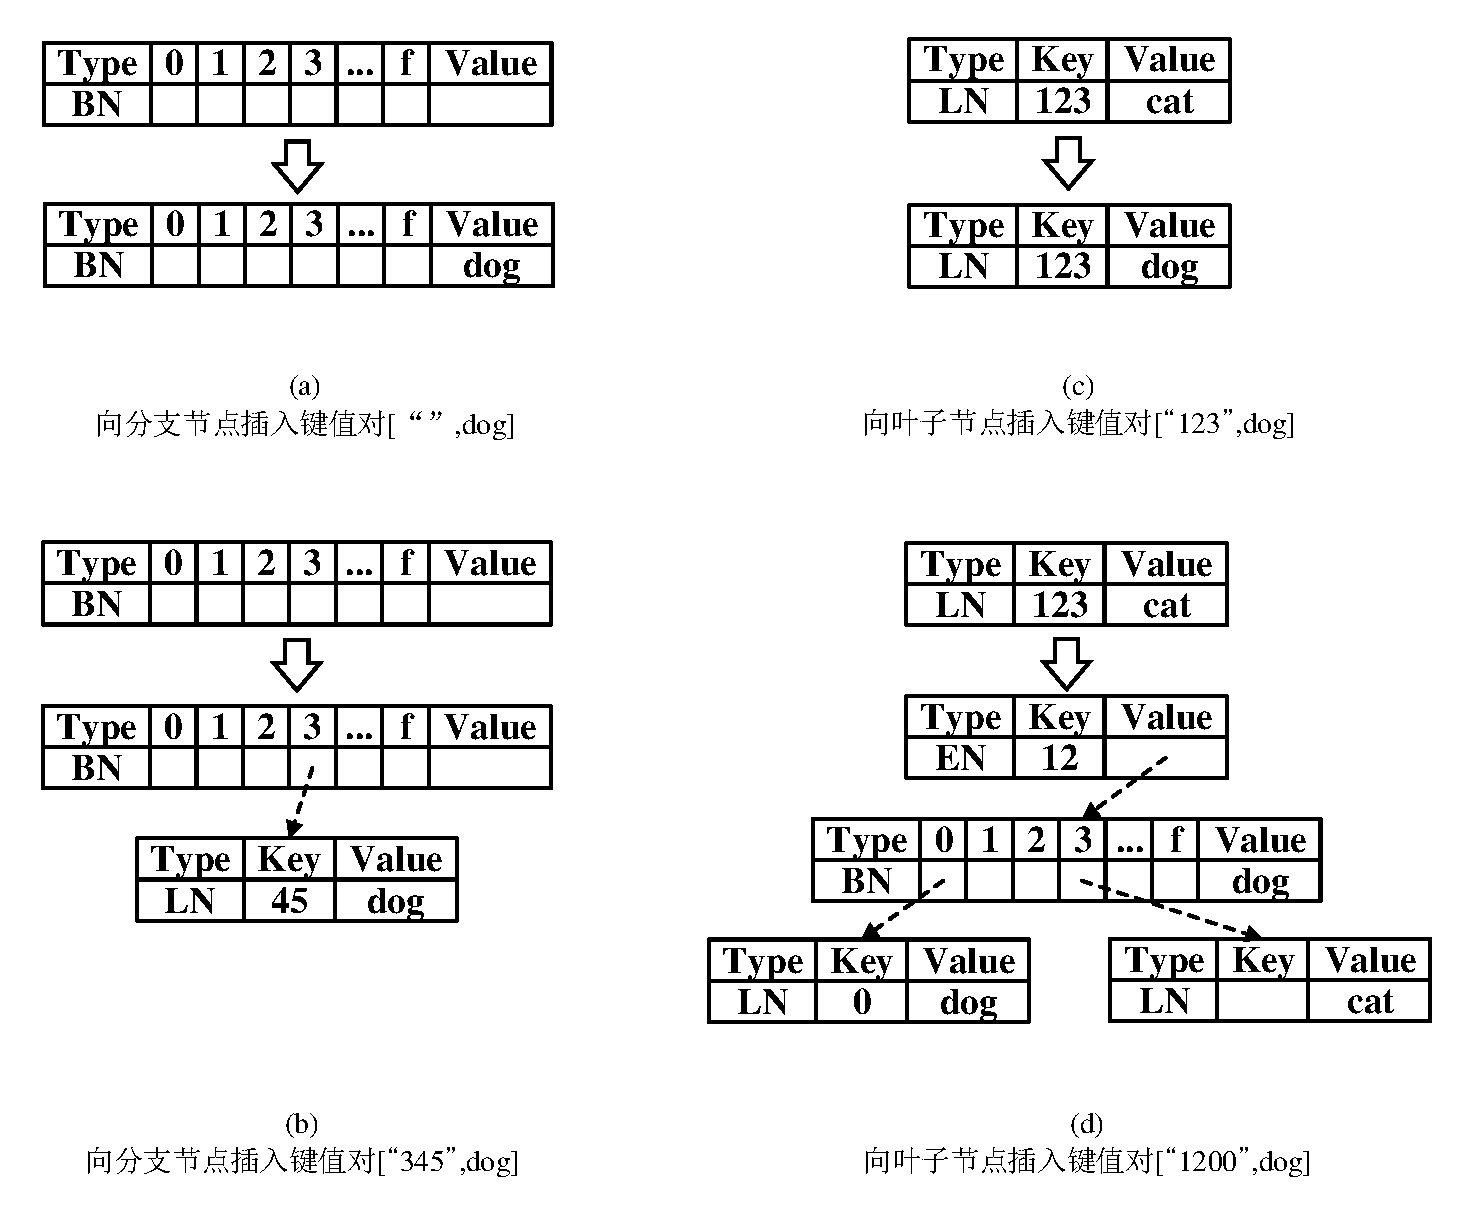
\includegraphics[width=6 in]{fig/MPTUpdate}
\DeclareGraphicsExtensions.
\caption{The Merkle Patricia Tree}
\label{fig:MPTUpdate}
\end{figure}

图~\ref{fig:MPTUpdate} 通过四个简单的例子展示了MPT树的插入过程。首先是将一个“键值对”插入到分支节点,这分为两种情况。如果当前的键空间已经为空,我们可以直接将“值”插入到分支节点的第17个位置。否则,在经过了分支节点匹配后,键空间中“剩余键”和“值”将会存储在分支节点指向的一个新的叶子节点中。其次是将“键值对”插入到叶子节点,也分为两种情况。如果当前键空间中“剩余键”与叶子节点中的“键”正好匹配,直接将叶子节点中的“值”修改为新的“值”即可。否则,我们将找到当前键空间“剩余键”和叶子节点“键”的共同前缀,将其作为一个新建的扩展节点的“键”,并新建一个分支节点,将现有的叶子节点和新建的叶子节点作为子节点插入到分支节点对应的空间中。

注意,MPT中的每一个节点都通过可递归长度前缀法~\cite{RLP_code}(Recursive Length Prefix, RLP) 进行了编码并对编码值再进行了哈希。数据库中存储了每个节点的“键值对”键值对,其中“键”为该节点RLP编码的哈希,“值”为该节点的RLP编码。这样每个节点可以通过他的哈希值被引用,同时保证了MPT的可搜索性和可验证性。通过这种方式,MPT的根哈希成为了整棵树的指纹信息,根哈希的值由所有下层节点的哈希值所决定,任何节点的微小改变都会导致根哈希的值发生变化。此外,MPT与默克尔树不同,MPT是完全确定性的,即一组相同的“键值对”采用不同的顺序插入到MPT中,最终得到的根节点哈希值是相同的,而默克尔树不具有这个性质。
%The Merkle Patricia Tree (MPT) is first proposed in Ethereum~ \cite{wood2014ethereum, merkle_patricia_tree}, which combines the Trie Tree and the Merkle Tree for data update efficiency. There are three kinds of nodes in an MPT to achieve the goal. Leaf Nodes(LN) represents [key,value] pairs. Extension Nodes(EN) represent [key,value] pairs where keys are the public prefixes and their values are the hashes of the next nodes. The Branch Nodes (BN) are used to store possible branches when the prefixes of the keywords differ, which is presented with 17 elements. Among the 17 elements, the first 16 elements represent the 16 possible hex characters in a key and the last element stores a value if a key in a [key,value] pair matches the node.

%Note that, each node of the MPT is represented by its hash and is encoded using Recursive Length Prefix (RLP) code that is mainly used to encode arbitrarily binary data~\cite{RLP_code}, which ensures the cryptographically security of the search operations. The root hash in MPT becomes a fingerprint of the entire tree and is computed based on all hashes of nodes below. Therefore, any modification in a node would incur recomputation of the root hash. Note that, the MPT is fully deterministic, meaning that an MPT with the same [key,value] pairs is exactly the same regardless of the order of insertion, which is different from the Merkle Tree.



%Searchable Encryption was first proposed by Song et al. \cite{song2000practical}, their solution allows a user to outsource its encrypted data to cloud services, and meanwhile retaining the ability to search over it. Normally, searchable encryption has been divided into two categories, i.e.,  Searchable Symmetric Encryption(SSE) and Public Key Encryption with keyword search(PKE). The most classical SSE scheme was proposed by Curtmola et al. in~\cite{curtmola2011searchable}. They defined  privacy against passive adversaries (i.e., honest but curious servers) and developed their scheme by using an inverted index. There exist various SSE schemes with different secure searching functionalities. For example, dynamic SSE schemes~\cite{kamara2012dynamic,cash2014dynamic,stefanov2014practical} allow a user to update his dataset and ranked keyword search scheme~\cite{wang2010secure} that allow a user to retrieve  ranked search results from the server. The most famous PKE scheme was proposed by Boneh et al.~\cite{boneh2004public} with the bilinear map. Normally, the efficiency of the PKE schemes are much lower than the SSE schemes.

%【SSE】Thanks for the suggestions. We explained the secure searchable encryption schemes in Section 2. Searchable encryption allows the server to perform search operations without seeing plaintext data. It empowers the server an ability to search over ciphertext and ensures the security of data on the server. In this revised manuscript, we discussed the existing categories of searchable encryption in Section 2.

\section{问题定义}
在本节中,我们将正式定义方案的攻击模型,方案需要解决的问题以及方案需要实现的目标。

\subsection{攻击模型}
在单用户场景中,数据持有者和数据搜索用户是同一人,而在多用户场景中,这两者是分开的。我们假定数据持有者本身是可信的,而数据搜索用户不可信。此外,我们假定提供存储和搜索服务的云服务器是不可信的,即 1) 云服务器会试图从用户的加密数据和搜索请求中推断出一些隐私信息; 2) 云服务器有可能会因为外部攻击、配置错误、软件错误等原因背离原有协议,从而导致产生数据新鲜性攻击和数据完整性攻击,用以节省其自身的计算开销和通信开销。数据新鲜性攻击和数据完整性攻击的正式定义如下:

\begin{definition}[\textbf{数据新鲜性攻击}]\label{def:freshness}
    {\itshape
			在对称加密搜索中,数据新鲜性攻击是指一个恶意的云服务器试图从旧数据集中返回搜索结果,而不从最新的数据集中返回搜索结果。正式地,让$\Delta_{n-1} = \{\delta_1,\delta_2,\cdots,\delta_{n-1}\}$ 代表用户数据集的历史版本, $\delta_n$ 代表用户的最新数据集,云服务器返回的搜索结果为 $\delta_i$ 的子集,其中 $1 \le i \le n-1$。
      %A data freshness attack in SSE is that a malicious server (or an attacker) attempts to return the historical version of the search result, not the most recently updated version. Formally, let $\Delta_{n-1} = \{\delta_1,\delta_2,\cdots,\delta_{n-1}\}$ denote the historical version of the dataset and $\delta_n$ is the latest version. However, the search result returned by the server is retrieved from $\delta_i$ where $1 \le i \le n-1$.
    }
\end{definition}

\begin{definition}[\textbf{数据完整性攻击}]\label{def:integrity}
    {\itshape
			在对称加密搜索中,数据完整性攻击是指一个恶意的云服务器试图篡改搜索结果,阻止数据搜索用户获取到完整的搜索结果。正式地,让 $\tau$ 代表对称加密搜索方案中的搜索令牌,$\delta_i$ 代表数据集,其中 $1 \le i \le n$。对应的搜索结果应为 $\mathcal{F}(\delta_i, \tau)$,但云服务器返回的搜索结果为 $\mathcal{G}(\delta_i, \tau)$, 其中$\mathcal{G}(\delta_i, \tau) \neq \mathcal{F}(\delta_i, \tau)$。
      %A data integrity attack in SSE is that a malicious server (or an attacker) attempts to tamper with the search result to prevent authenticated users from accessing the complete and correct search result. Formally, let $\tau$ be the search token of the SSE scheme, and $\delta_i$ be the dataset, where $1 \le i \le n$, the corresponding search result should be $\mathcal{F}(\delta_i, \tau)$, but the result returned by the server is $\mathcal{G}(\delta_i, \tau)$, where $\mathcal{G}(\delta_i, \tau) \neq \mathcal{F}(\delta_i, \tau)$.
    }
\end{definition}

%We assume that the data owner is trusted and the data users authorized by the data owner are also trusted\footnote{Please refer to Section \ref{Sec:Discussion} for details on how we can enforce such assumption in practice with multi-user access control techniques.}.
%We consider cloud services performing searchable symmetric encryption (SSE) to be untrusted, which means 1) cloud services intends to derive some sensitive information from the encrypted data and the queries; 2) cloud services may deviate from the prescribed protocols and mount a data freshness attack or a data integrity attack to save its computation or communication cost. The definitions of the data freshness attack and the data integrity attack are presented as follow:

%在可验证加密搜索中,由于服务器不诚信导致的安全性攻击主要可以分为以下两种:
%	重放攻击(Replay Attack):在加密搜索中,重放攻击是指服务器(攻击者)试图返回旧的搜索结果,而不是最新的搜索结果。我们用Δ_n={δ_1,δ_2,⋯,δ_n}来表示旧版本的数据集,用δ_(n+1)来表示最新的数据集,则服务器返回的搜索结果是数据集δ_i的搜索结果,其中1≤i≤n。
%	数据完整性攻击(Data Integrity Attack):在加密搜索中,数据完整性攻击是指服务器(攻击者)试图不让用户获取完整的搜索结果。我们用τ来表示加密搜索中用户的搜索陷门,用户应该得到的搜索结果为F(τ),而服务器返回的搜索结果为G(τ),其中G(τ)⊂F(τ)并且G(τ)可能为∅。
%重放攻击仅存在于动态的加密搜索方案中,在数据库静态的情况下不存在。但现实中,动态数据库较为常见,因此重放攻击是可验证加密搜索必须要解决的问题。数据完整性攻击不仅包括服务器少返回搜索结果的情况还包括了服务器不返回搜索结果来规避结果验证的情况。


\subsection{设计目标}

本论文旨在设计一种普适的可验证加密搜索框架,即该方案可以和任意加密搜索方案相结合,包括但不限于~\cite{stefanov2014practical,cash2014dynamic,kamara2012dynamic},使其能够完成结果验证的功能。本方案将现有的加密搜索方案当做黑盒,总体来说,需要满足以下几个需求:

\begin{enumerate}
	\item \textbf{机密性:} 数据和关键字的机密性是加密搜索最近本的安全需求。它保证了用户的明文数据和关键字信息无法被其他不可信第三方所推断。并且保证了敌手无法从方案的加密数据集,验证索引以及搜索关键字中推断出任何有用的隐私信息。
	%The confidentiality of data and keywords is the most important privacy requirements in SSE. It ensures that users' plaintext data and keywords cannot be revealed by any unauthorized parties, and an adversary cannot learn any useful information about files and keywords through the proof index and update tokens used in %\name.
	%In our scheme, data privacy and keyword privacy is guaranteed by its underlying cipher. Moreover, the search pattern of our scheme is hiding by trading the space.
	\item \textbf{可验证性:} 一个可验证的对称加密搜索方案应该能够验证搜索结果的正确性和完整性,即防止重放攻击和数据完整性攻击。%A verifiable SSE scheme should be able to verify the freshness and integrity of the search results for users.
	%In our scheme, we design a proof algorithm based on the proof structure to detect the dara integrity attacks and meanwhile use the chained-timestamp mechanism to detect the replay attacks.
	\item \textbf{高效性:} 一个可验证对称加密搜索方案应该达到次线性的计算复杂度,即对数复杂度 $O(log(|W|))$,其中 $|W|$ 是关键字的总数,并且应该在支持用户数据更新的情况下仍然能达到该复杂度。注意,这里的计算复杂度仅仅指服务器提供结果验证服务时所需的额外计算复杂度,不包括加密搜索方案本身带来的计算复杂度。%A verifiable SSE scheme should achieve sublinear computational complexity, e.g. logarithmic $O(log(|W|))$, where $|W|$ is the number of keywords, even with file update. Note that, the computational complexity only refers to the cost of searching operations for verification, which does not include the complexity of the searching operations in the existing SSE schemes.
	%Update efficiency, search efficiency and verification efficiency is the most improtant indicator we aim to achieve. In our scheme, we leverage the Mekle Patricia Tree (MPT) which provides the $O(log(n))$ efficiency for search and update which is the optimal solution to the best of our knowledge.
\end{enumerate}

	%机密性:数据和关键字机密性是加密搜索中最重要的隐私需求。其中,数据机密性要求用户的明文数据不能被云服务器获取,关键字机密性要求关键字和文件的相关性不能被云服务器所推断。
	%可验证性:一个可验证的加密搜索方案应该能够验证搜索结果的正确性和完整性,即防止重放攻击和数据完整性攻击。
	%效率:一个可验证的加密搜索方案应该在搜索和更新时具有合理的计算复杂度,例如O(log⁡(|W|)),其中|W|是关键字的数目。


  %This paper aims to provide result verification for any SSE schemes, including but not limited to~\cite{stefanov2014practical,cash2014dynamic,kamara2012dynamic}. Therefore, we treat an existing SSE scheme as a black box such that our proposed scheme can be applied to these SSE schemes for result verification.

\chapter{单用户下的可验证对称加密搜索方案研究}
\label{cha:single-user}
\section{引言}
本章提出了一种通用的可验证对称加密搜索方案\single,该方案可以在单用户场景下工作,与任意对称加密搜索方案结合后,可以为用户提供加密搜索的结果验证服务。本章的主要内容如下:首先介绍了单用户场景下(即数据持有者为数据搜索用户本身)的系统架构,介绍了该框架的参与方及其所承担的计算任务;接着,通过一个正式定义从抽象层面介绍了该框架工作的流程和每个参与方涉及到的算法。随后,对\single 方案涉及到的算法进行了详细分析,包括数据持有者构建和更新验证索引的算法,云服务器搜索验证索引并生成结果证明的算法,数据持有者进行结果验证的算法。随后通过一个简单的例子对这几个算法进行了详细的阐述。最后,通过安全性分析和实验结果分析证明\single 方案可以达到设计目标中的安全性要求和性能要求。

\section{系统架构}
单用户场景下的可验证对称加密搜索方案系统架构如图~\ref{fig:GS-VSSE}所示,数据持有者即为数据搜索用户本身。初始化时需要数据持有者对自身的数据集进行加密,并对该数据集构建加密的验证索引,用于后续结果验证。数据持有者将该验证索引上传给云服务器存储,并在需要时更新验证索引。当用户需要进行关键字搜索时,他将会构建出一个与关键字相关的搜索令牌,提交给云服务器进行搜索。云服务器接收到该搜索令牌后,通过某个加密搜索方案取得加密搜索结果,同时通过搜索验证索引取得一个针对于该搜索结果的结果证明,最后云服务器将结果证明返回给用户。用户在收到该结果证明和加密搜索方案提供的搜索结果后,对搜索结果进行结果验证,若验证失败,则丢弃该结果。
\begin{figure}[t]
\centering
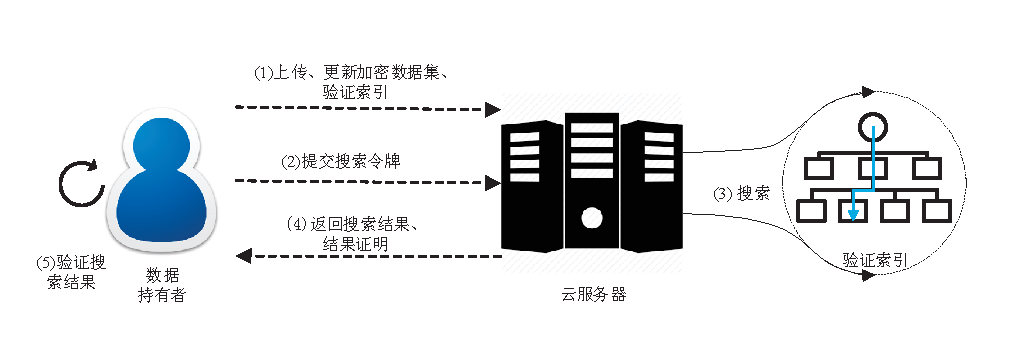
\includegraphics[width=6 in]{fig/GS-VSSE}
\DeclareGraphicsExtensions.
\caption{单用户场景下的可验证对称加密搜索框架\single}
\label{fig:GS-VSSE}
\end{figure}


\section{方案流程}
由于\single 方案的主要目标是为对称加密搜索方案提供结果验证功能,因此在开始讲述\single 方案的流程前,我们先回顾对称加密搜索方案的常见定义,如定义\ref{def:SSE}所示。
\begin{definition}[\textbf{SSE} 方案]\label{def:SSE}
  {\itshape
    一个支持文件更新的$SSE$方案,参与方包括两个,分别为数据持有者本身和半可信的云服务器。数据持有者向云服务器提供加密数据集和搜索索引,使得云服务器可以在密文上进行搜索,从而同时确保数据的可搜索性和隐私性。一个$SSE$方案可以定义为如下六个算法的集合:
    \begin{itemize}
      \item $KGen_{\mathcal{SSE}}(1^k) \rightarrow \{\mathcal{K}\}$: 是由数据持有者执行的秘钥生成算法。它将一个安全参数作为输入,输出一系列对称秘钥$\mathcal{K}$。
      \item $Init_{\mathcal{SSE}}(\mathcal{K}, \mathcal{D}) \rightarrow \{\gamma, \mathcal{C}\}$: 是由数据持有者执行的初始化算法。它将对称秘钥$\mathcal{K}$和明文文件集$\mathcal{D}$作为输入,输出搜索索引$\gamma$和密文文件集$\mathcal{C}$。数据持有者将搜索索引$\gamma$和密文文件集$\mathcal{C}$上传给云服务器。
      \item $UpdateToken_{\mathcal{SSE}}(\mathcal{K}, d) \rightarrow \{\tau_u\}$: 是由数据持有者执行的更新令牌生成算法。它将对称秘钥$\mathcal{K}$和需要更新的文件$d$作为输入,输出一系列更新令牌$\tau_u$。数据持有者将更新令牌$\tau_u$上传给云服务器。
      \item $Update_{\mathcal{SSE}}(\gamma, \tau_u) \rightarrow \{\gamma'\}$: 是由云服务器执行的更新算法。它将搜索索引$\gamma$和更新令牌$\tau_u$作为输入,输出更新后的搜索索引$\gamma'$。
      \item $SearchToken_{\mathcal{SSE}}(\mathcal{K}, w) \rightarrow \{\tau_{w}\}$: 是由数据持有者执行的搜索令牌生成算法。它将对称秘钥$\mathcal{K}$和某一关键字$w$作为输入,输出与该关键字相关搜索令牌$\tau_{w}$。数据持有者将该搜索令牌 $\tau_{w}$上传给云服务器进行搜索。
      \item $Search_{\mathcal{SSE}}(\gamma, \tau_{w}) \rightarrow \{C_w\}$: 是由云服务器执行的搜索算法。它将搜索索引$\gamma$和搜索令牌$\tau_{w}$作为输入,输出搜索结果$C_w$。云服务器将搜索结果$C_w$返回给数据持有者。
    \end{itemize}
  }
\end{definition}

在定义\ref{def:SSE}中,$SSE$算法对云服务器的假定为半可信的,即云服务器不会违背协议本身。因此在$SSE$方案中,云服务器在通过$Search$算法将搜索结果返回给用户后,用户无条件的接受该结果作为正确结果。然而在现实情况中,这种对云服务器半可信的假定往往是不成立的,云服务器往往会因为一些外部攻击,甚至配置错误、软件错误等原因背离原有协议,产生恶意行为。因此我们需要设计一个方案来对搜索结果进行验证,以确保云服务器没有恶意行为。\single 方案即在上述$SSE$的基础上,为其提供了一套结果验证机制。该机制可以与$SSE$方案中的每一个算法并行操作,在为其进行结果验证的同时,保证了整体方案的高效性。\single 方案的具体算法如定义~\ref{def:single}所示。

\begin{definition}[\textbf{\single 方案}]\label{def:single}
  {\itshape
      在\single 方案中,参与方有两个,分别为数据持有者本身和不可信的云服务器。数据持有者向云服务器提供验证索引,使得云服务器在用户搜索时可以向其返回结果证明,用于确保加密搜索结果的新鲜性和完整性。一个\single 方案是以下八个算法的集合:
      \begin{itemize}
        \item $KGen(1^k) \rightarrow \{K_1,K_2\}$: 是由数据持有者执行的秘钥生成算法。它将一个安全参数作为输入,输出对称秘钥$K_1,K_2$。
        \item $Init(K_1,K_2, \mathcal{D}) \rightarrow \{\lambda\}$: 是由数据持有者执行的初始化算法。它将对称秘钥$K_1,K_2$和明文文件集$\mathcal{D}$作为输入,输出验证索引$\lambda$。数据持有者在本地保存验证索引$\lambda$的根节点哈希$rt$,并将验证索引$\lambda$上传给云服务器。
        \item $UpdateToken(K_1,K_2, d) \rightarrow \{\tau_u\}$: 是由数据持有者执行的更新令牌生成算法。它将对称秘钥$K_1,K_2$和需要更新的文件$d$作为输入,输出一系列更新令牌$\tau_u$。数据持有者将更新令牌$\tau_u$上传给云服务器。
        \item $Update(\lambda, \tau_u) \rightarrow \{\lambda',\rho_u\}$: 是由云服务器执行的更新算法。它将验证索引$\lambda$和更新令牌$\tau_u$作为输入,输出更新后的验证索引$\lambda'$和更新证明$\rho_u$。云服务器将更新证明$\rho_u$返回给用户。
        \item $VerifyUpdate(rt,\tau_u,\rho_u) \rightarrow \{rt'\}$:是由数据持有者执行的更新算法。它将验证索引$\lambda$的根哈希 $rt$,更新令牌$\tau_u$和服务器返回的更新证明 $\rho_u$ 作为输入,输出新的根哈希$rt'$。若更新证明$\rho_u$验证通过,则输出更新后的根哈希$rt'$,若更新证明验证失败,则输出的根哈希$rt'$与原始根哈希$rt$相同。
        \item $SearchToken(K_1, w) \rightarrow \{\tau_{w}\}$: 是由数据持有者执行的搜索令牌生成算法。它将对称秘钥$K_1$和某一关键字$w$作为输入,输出与该关键字相关搜索令牌$\tau_{w}$。数据持有者将该搜索令牌 $\tau_{w}$上传给云服务器进行搜索。
        \item $Prove(\lambda, \tau_{w}) \rightarrow \{\rho_s\}$: 是由云服务器执行的结果证明生成算法。它将验证索引$\lambda$和搜索令牌$\tau_{w}$作为输入,输出结果证明$\rho$。云服务器将结果证明$\rho$返回给数据持有者。
        \item $Verify(K_1,K_2, C_w, \rho_s,\tau_{w}, rt) \rightarrow \{b\}$: 是由数据持有者执行的验证算法。它将对称秘钥$K_1,K_2$,加密搜索结果$C_w$,结果证明$\rho_s$,搜索令牌$\tau_{w}$和保留的验证索引根哈希$rt$作为输入,输出一个比特$b$,代表接受或者拒绝该搜索结果。
      \end{itemize}
      }
\end{definition}

注意,上述流程中的每一个算法(除了$VerifyUpdate$,$Verify$算法),都与加密搜索流程中的算法一一对应。例如$KGen$,$Init$,$UpdateToken$,$Update$,$SearchToken$算法都可以与加密搜索中的秘钥生成,初始化,更新令牌生成,更新操作以及搜索令牌生成同时进行,而$Prove$算法则可以与加密搜索方案中的$Search$搜索操作同时进行。该可验证加密搜索方案带来的额外算法是$VerifyUpdate$和$Verify$算法,它们分别用于用户收到更新结果和搜索结果后的验证操作。正是因为\single 方案的每一个算法都从加密搜索方案中解耦了出来,才使得该方案可以将加密搜索方案当做黑盒,并为任意加密搜索方案提供结果验证服务。

\section{方案设计}
在本节,我们将具体阐述\single 方案,即单用户场景下的可验证加密搜索方案。我们将详细讲解定义~\ref{def:single}中的算法。首先我们将描述如何通过$Init$算法来建立验证索引,并通过$Update$算法和$VerifyUpdate$算法来阐述如何更新验证索引。然后我们将通过$Prove$算法给出服务器生成结果证明的方法,并通过$Verify$算法详细解释用户如何利用结果证明来确保搜索结果的正确性。最后,我们将通过一个简单的例子来详细说明上述算法的执行流程,以便于读者理解。

\subsection{构建及更新验证索引}

算法~\ref{alg:Init} 给出了建立验证索引的伪代码。首先数据持有者根据明文文件集$\mathcal{D}$计算出倒排索引$\Delta$,其中倒排索引$\Delta$是指关键字$w_i$与包含该关键字的文件$D_{w_i}$组成的索引。对倒排索引中的每一个关键字$w_i$,我们计算他的"键值对",其中“键”是每一个关键字通过伪随机函数生成的令牌,而“值”是包含该关键字的文件的增量哈希和。我们通过将这些“键值对”插入MPT中来形成验证索引。
\begin{algorithm}[ht]
  \caption{$Init$ 算法}
  \label{alg:Init}
  \begin{algorithmic}[1]
    \REQUIRE ~~{$K_1,K_2$: 对称秘钥; $\mathcal{D}$: 明文文件集合;  $F, G: \{0, 1\}^k \times \{0, 1\}^* \rightarrow \{0, 1\}^*$ 伪随机函数; $IH: \{0, 1\}^* \rightarrow \{0, 1\}^k$ 增量哈希函数; $H: \{0, 1\}^* \rightarrow \{0, 1\}^k$ 哈希函数}
    \ENSURE ~~{$\lambda$: 通过MPT构建的验证索引。}
              \FOR {each $w_i \in \Delta$, 其中 $\Delta$ 是包括了$<w_i, D_{w_i}>$ 的明文倒排索引, $i \in \{1,\cdots, |W|\}$。}
                \STATE{生成“键”:$\tau_{w_i} = F_{K_1}(w_i)$。}
                \STATE{生成“值”:$V_{w_i} = \sum_{d \in D_{w_i}}IH (G_{K_2} (d))$。}
                \STATE{向MPT中插入键值对 $(\tau_{w_i},V_{w_i})$。}
              \ENDFOR
              \RETURN 返回从MPT构建得到的验证索引 $\lambda$。
  \end{algorithmic}
\end{algorithm}


对验证索引的更新操作支持三种方式,即插入、删除和编辑文件,其中编辑文件相当于删除一个文件后再新增一个文件。对于插入新文件操作,我们首先解析该文件$d$,得到该文件包含的关键字集合$W_d$,对每一个关键字$w_i \in W_d$,我们都用伪随机函数生成他的令牌$\tau_{w_i }$,并将文件的伪随机结果$G_{K_2}(d)$同时上传给云。如算法~\ref{alg:update}所示,云服务器在收到后更新令牌$\tau_u$后,首先需要将更新令牌$\tau_u$解析为键值对($\tau_{w_i}$,$G_{K_2}(d)$),并通过更新令牌$\tau_{w_i}$找到对应的叶子节点,将$IH(G_{K_2}(d))$与原有的叶子节点的值相加。如果该令牌对应的叶子节点尚不存在,则需要为其创建一个新的叶子节点,并将剩余键$remain\_key$和对应的值$IH(G_{K_2}(d))$作为键值对插入其中。删除操作同样,只是将原有的叶子节点的值减去$IH(G_{K_2}(d))$。此外,云服务器在更新每一个令牌时,都需要将该令牌对应的搜索路径$\sigma_{w_i}$保存在更新证明$\rho_u$中,用于后续发回给用户进行更新验证。


\begin{algorithm}[ht]
  \caption{$Update$ 算法}
  \label{alg:update}
  \begin{algorithmic}[1]
    \REQUIRE ~~{$\lambda$: 验证索引; $\tau_u$:更新令牌;}
    \ENSURE ~~{$\lambda'$: 更新后的验证索引;$\rho_u$: 更新证明;}
              \STATE{将更新令牌$\tau_u$解析为键值对($\tau_{w_i}$,$G_{K_2}(d)$),其中$i \in \{1,\cdots,|W_d|\}$,$d$为待更新的文件。}
              \FOR {each $\tau_{w_i} \in \tau_u$}
                \STATE{将$\tau_{w_i}$在$\lambda$中进行路径匹配,将$\tau_{w_i}$匹配后剩余的后缀作为$remain\_key$。}
                \IF{$remain\_key = \emptyset$,即$\tau_{w_i} \in \lambda$}
                  \STATE{将$IH(G_{K_2}(d))$更新到$\tau_{w_i}$到对应的叶子节点。}
                  \STATE{将$\tau_{w_i}$在$\lambda$上的搜索路径$\sigma_{w_i}$添加到更新证明$\rho_u$中。}
                \ELSIF{$remain\_key != \emptyset$,即$\tau_{w_i} \notin \lambda$}
                  \STATE{根据MPT更新规则,将$(remain\_key,IH(G_{K_2}(d)))$作为键值对插入到新建的叶子节点中。}
                  \STATE{将$\tau_{w_i}$在$\lambda$上的搜索路径$\sigma_{w_i}$添加到更新证明$\rho_u$中。}
                \ENDIF
              \ENDFOR
              \RETURN{返回更新证明$\rho_u$。}
  \end{algorithmic}
\end{algorithm}



算法~\ref{alg:verifyupdate}展示了数据持有者在收到云服务器返回的更新证明$\rho_u$后,执行的更新验证操作,该操作确保了数据的新鲜性。由于数据持有者本身在本地并不保留验证索引$\lambda$,只保留验证索引的根哈希$rt$,因此在数据产生更新时,如何更新该根哈希$rt$十分重要。因为云服务器是不可信的,数据持有者在提交了更新令牌$\tau_u$后,无法确保服务器执行了正确的更新操作,因此他需要云服务器返回更新证明$\rho_u$来进行验证,并且根据更新证明来更新根哈希$rt$。服务器返回的更新证明$\rho_u$包含了更新令牌中每一个关键字令牌$\tau_{w_i}$对应在验证索引$\lambda$上的路径$\sigma_{w_i}$。用户在接受到该更新证明后,首先将自身生成的更新令牌$\tau_u$解析为($\tau_{w_i}$,$G_{K_2}(d)$),将更新证明$\rho_u$解析为键值对$\sigma_{w_i}$。随后对每一个令牌$\tau_{w_i}$,验证是否能根据$\sigma_{w_i}$生成原始根哈希$rt$。若每个令牌都能验证成功,则用户通过更新令牌$\tau_u$和更新验证$\rho_u$构建新的根哈希$rt'$,否则验证失败,用户保留原有根哈希$rt$。


\begin{algorithm}[ht]
  \caption{$VerifyUpdate$ 算法}
  \label{alg:verifyupdate}
  \begin{algorithmic}[1]
    \REQUIRE ~~{$rt$: 验证索引的根哈希; $\tau_u$:更新令牌;$\rho_u$: 更新证明;}
    \ENSURE ~~{$rt'$: 更新后的根哈希。}
              \STATE{将更新令牌$\tau_u$解析为键值对($\tau_{w_i}$,$G_{K_2}(d)$),其中$i \in \{1,\cdots,|W_d|\}$,$d$为待更新的文件。}
              \STATE{将更新证明$\rho_u$解析为键值对$\sigma_{w_i}$,其中$i \in \{1,\cdots,|W_d|\}$。}
              \FOR {each $\tau_{w_i} \in \tau_u$}
                \STATE{根据更新令牌$\tau_{w_i}$和更新证明$\sigma_{w_i}$重构出根哈希$rt_t$。}
                \IF{$rt_t \neq rt$}
                  \RETURN{验证失败,返回原有根哈希$rt$。}
                \ENDIF
              \ENDFOR
              \STATE{根据更新令牌$\tau_u$和更新证明$\rho_u$重构出根哈希$rt'$}
              \RETURN{更新后的根哈希 $rt'$。}
  \end{algorithmic}
\end{algorithm}

在本章第\ref{sec:example}节,我们将通过一个例子来说明建立和更新验证索引的过程。


\subsection{生成结果证明}
如算法~\ref{alg:Prove}所示,服务器根据用户提交的搜索令牌$\tau_{w_i}$和验证索引$\lambda$来生成结果证明$\rho_s$。首先服务器根据搜索令牌$\tau_{w_i}$来寻找搜索路径$\sigma_{w_i}$。如果搜索令牌$\tau_{w_i}$对应的叶子节点存在,即用户查询的关键字存在,则服务器从叶子节点的上一层节点开始,返回搜索路径上的“键”作为结果证明。注意对于分支节点,服务器还需要返回不在搜索路径上的“键值对”。如果搜索令牌$\tau_{w_i}$对应的叶子节点不存在,即用户查询的关键字不存在,则服务器需要从搜索终结的节点开始自底向上返回搜索路径中的“键”作为结果证明,而对于搜索的终结节点,服务器需要返回完整的键值对。
我们将在本章第\ref{sec:example}节,通过一个具体的例子来说明该过程。

\begin{algorithm}[ht]
  \caption{$Prove$算法}
  \label{alg:Prove}
  \begin{algorithmic}[1]
    \REQUIRE {$\lambda$: 云服务器维护的验证索引; $\tau_{w_i}$: 用户提交的搜索令牌; }
    \ENSURE {$\rho_s$: 搜索结果的结果证明;}
              \STATE {查找搜索令牌$\tau_{w_i}$在验证索引$\lambda$上的对应路径 $\sigma_{w_i} =(n_0, \cdots, n_i, \cdots, n_m)$,直到匹配到叶子节点或者匹配失败,其中 $n_i \in \{EN, BN, LN\}$, $n_0$ 为根节点。}
              \IF {$t_{w_i}$ 在验证索引$\lambda$中存在}
                \FOR {$i = m-1$ to $0$}
                  \IF {$n_i = BN$}
                    \STATE {$\rho_s = \rho_s \cup C_{n_i}$,其中 $C_{n_i}$ 包括分支节点中在搜索路径 $\sigma$ 上的"键"和不在搜索路径上的“键值对”。}
                  \ELSIF{$n_i = EN$}
                    \STATE {$\rho_s = \rho_s \cup C_{n_i}$,其中 $C_{n_i}$ 包括扩展节点中的“键”。}
                  \ELSE
                    \STATE{$\rho_s = \rho_s \cup C_{n_i}$,其中 $C_{n_i}$ 包括叶子节点中的“键值对”。}
                  \ENDIF
                \ENDFOR
              \ELSE %{$t_{w_i}$ not exits}
                \FOR {$i = m$ to $0$}
                    \STATE{重复步骤 4-10}
                \ENDFOR
              \ENDIF
              \RETURN{$\rho_s$}
  \end{algorithmic}
\end{algorithm}

\subsection{结果验证}

\begin{algorithm}[t]
  \caption{$Verify$算法}
  \label{alg:verify}
  \begin{algorithmic}[1]
    \REQUIRE {$K_1,K_2$: 对称秘钥; $C_{w}$: 加密搜索结果; $\rho_s$: 加密搜索结果证明; $\tau_{w}$: 用户提交的搜索令牌;$rt$:用户本身保留的根哈希;}
    \ENSURE {$b \in \{0,1\}$, 如果 $b=1$, 表示结果验证成功,否则表示结果验证失败;}
          \STATE {将$\tau_{w_i}$与结果证明$\rho_s$中的键进行匹配,得到剩余键 $remain\_key$。}
          \STATE{如果$\rho_s$中的某条路径是$\tau_{w_i}$的前缀,则$remain\_key$为$\tau_{w_i}$匹配后的剩余键;否则$remain\_key = \emptyset$。}
          \IF {$C_{w} = \emptyset$ \&\& $remain\_key = \emptyset$}
              \STATE {根据结果证明$\rho_s$自底向上计算根哈希$rt_t$;}
          \ELSIF {$C_{w} \neq \emptyset$ \&\& $remain\_key \neq \emptyset$}
              \STATE {计算 $\varphi = \sum_{d \in D_{w}}IH (G_{K_2} (d))$, 其中 $D_w$ 是 $C_w$ 对应的明文信息;}
              \STATE {计算叶子节点 $LN = Compute(\varphi, remain\_key)$}
              \STATE {根据结果证明 $\rho$ 和叶子节点$LN$ 自底向上计算根哈希$rt_t$.}
          \ELSE
              \RETURN {$0$}
          \ENDIF
          \IF{$rt = rt_t$}
            \RETURN{$1$}
          \ELSE
            \RETURN{$0$}
          \ENDIF
  \end{algorithmic}
\end{algorithm}

如算法~\ref{alg:verify} 所示,当用户收到了结果证明$\rho_s$时,就可以开始验证数据的完整性。首先用户通过搜索令牌$\tau_{w_i}$与结果证明$\rho_s$中的“键”进行匹配。如果结果证明$\rho_s$中的“键”是搜索令牌$\tau_{w_i}$的前缀,则$remain\_key$存储搜索令牌$\tau_{w_i}$与结果证明匹配完后剩余的键。如果结果证明$\rho_s$中的“键”不是搜索令牌$\tau_{w_i}$的前缀,那么$remain\_key$就置为$\emptyset$。如果搜索结果 $C_{w}$ 和 $remain\_key$ 都为空集,即云服务器返回了空搜索结果,则我们通过结果证明$\rho_s$直接计算出根哈希值$rt_t$。如果二者都不为空,则我们首先通过搜索结果$C_{w}$和$remain\_key$生成叶子节点的哈希值,再通过结果证明$\rho_s$重建出根哈希值$rt_t$。除了这两种情况以外,我们就认为服务器故意返回了空结果或服务器篡改了结果证明的内容。最后,用户通过对比重建得到的根哈希$rt_t$和用户本身保留的根哈希$rt$是否相等来判断数据完整性。如果二者相等,则验证通过,如果二者不相等,则说明服务器少返回了搜索结果或者服务器篡改了结果证明。



\subsection{实例分析}
\label{sec:example}

\begin{figure}[ht]
\centering
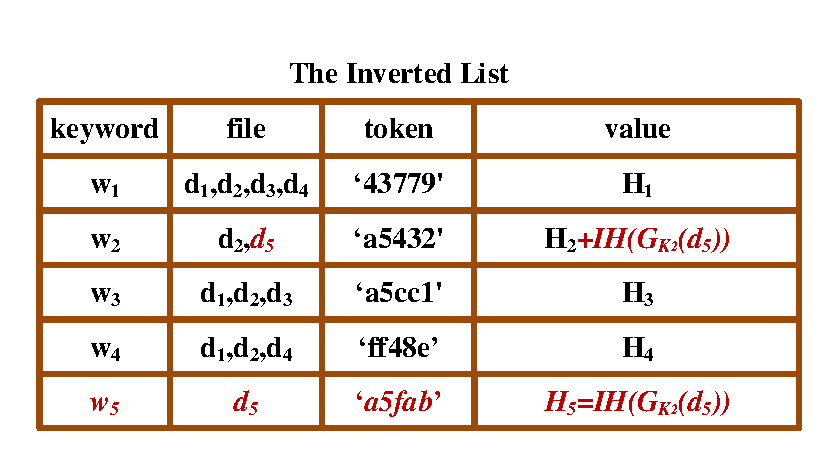
\includegraphics[width=4 in]{fig/inverted-index}
\DeclareGraphicsExtensions.
\caption{一个简单的倒排索引}
\label{fig:inverted-index}
\end{figure}

\begin{figure}[ht]
\centering
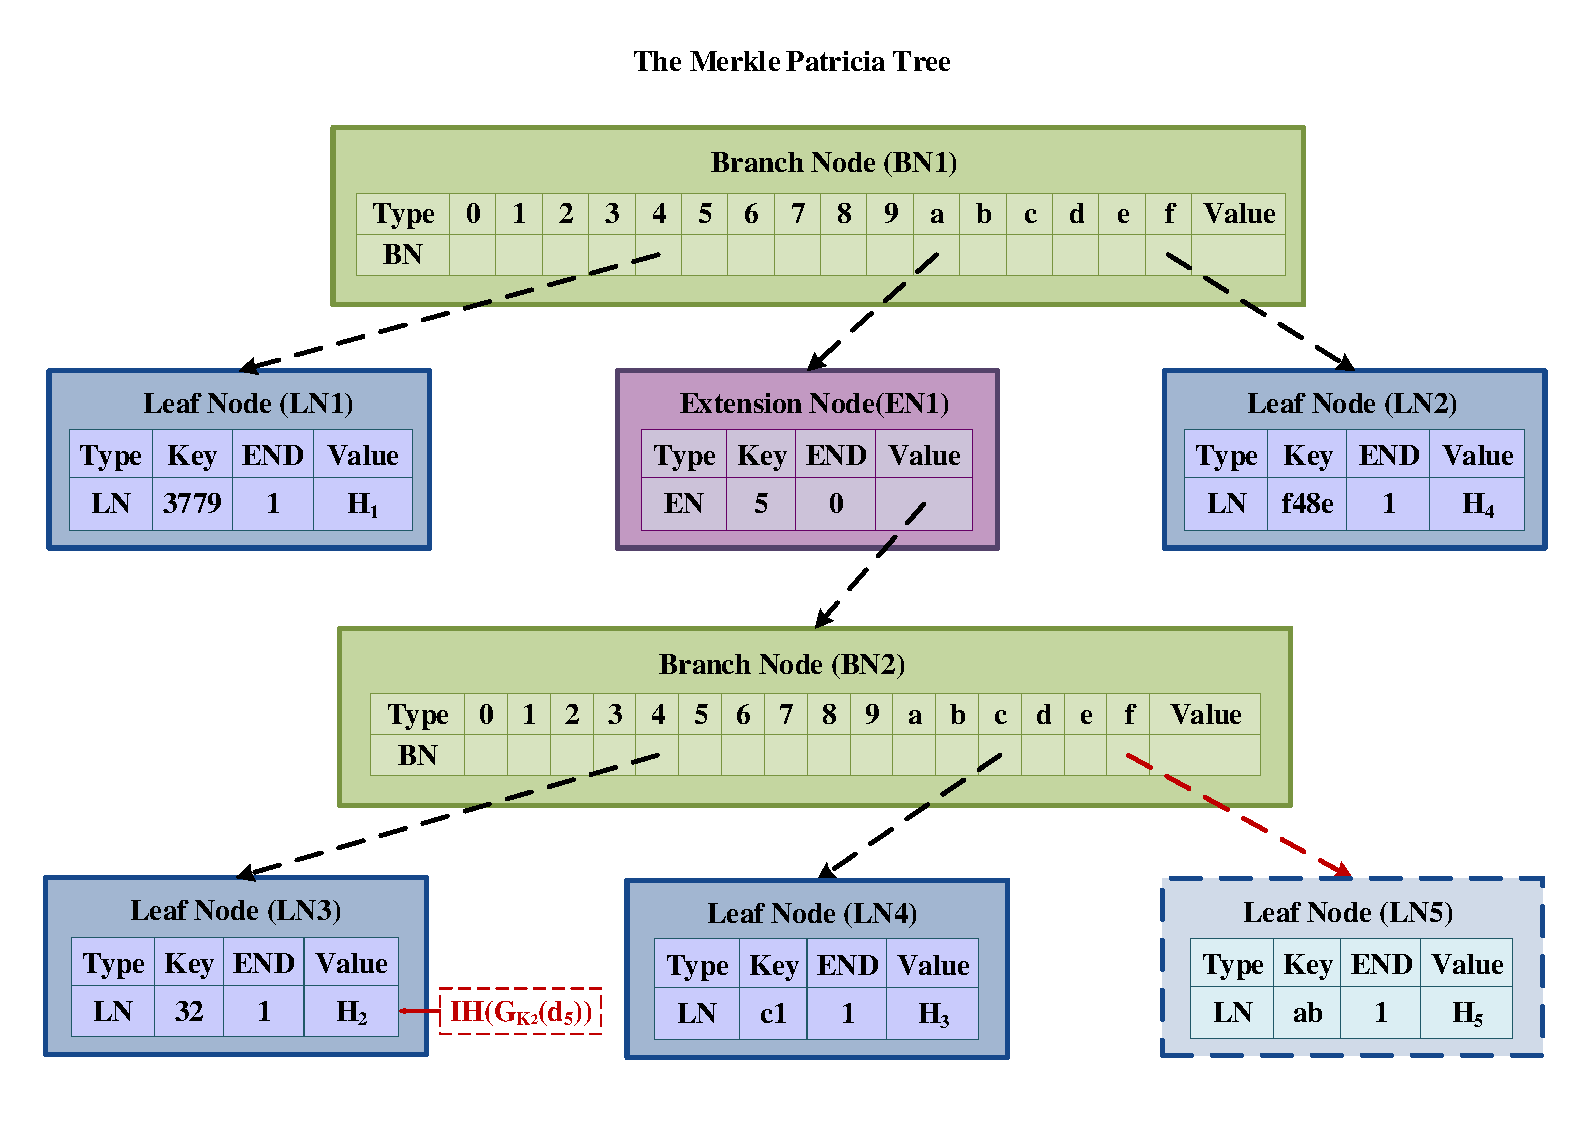
\includegraphics[width=6 in]{fig/MPT}
\DeclareGraphicsExtensions.
\caption{由倒排索引和MPT构建的验证索引}
\label{fig:MPT}
\end{figure}


\begin{figure}[ht]
  \begin{minipage}[b]{0.49\textwidth}
    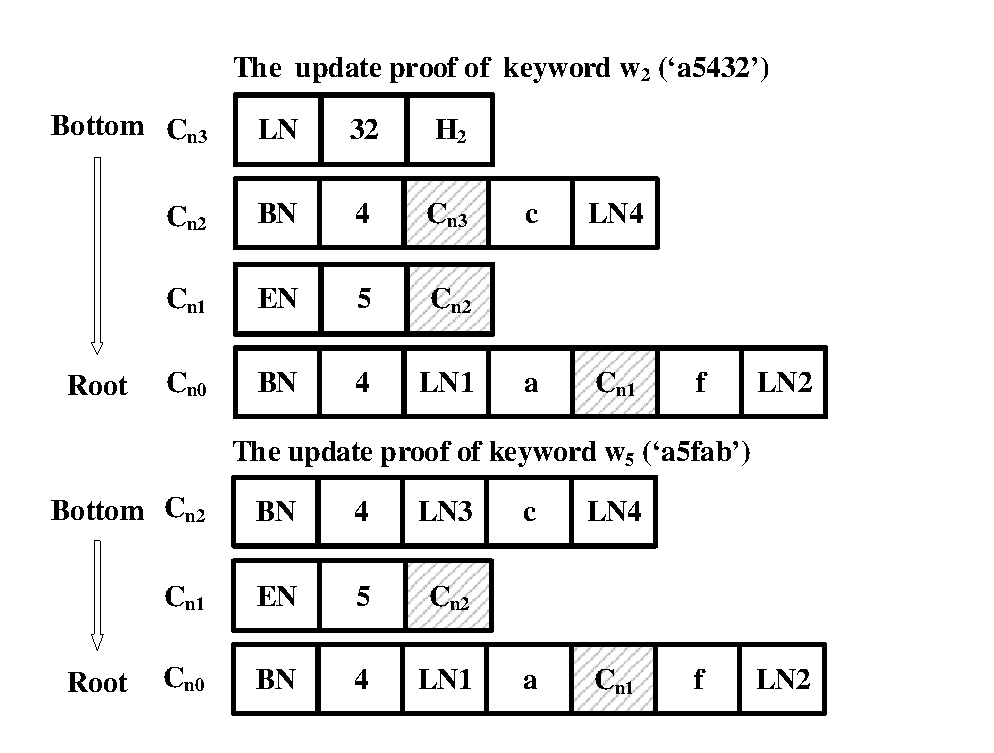
\includegraphics[width= 2.9 in]{fig/updateProof}
    \caption{更新证明}
    \label{fig:updateProof}
  \end{minipage}
  \begin{minipage}[b]{0.49\textwidth}
    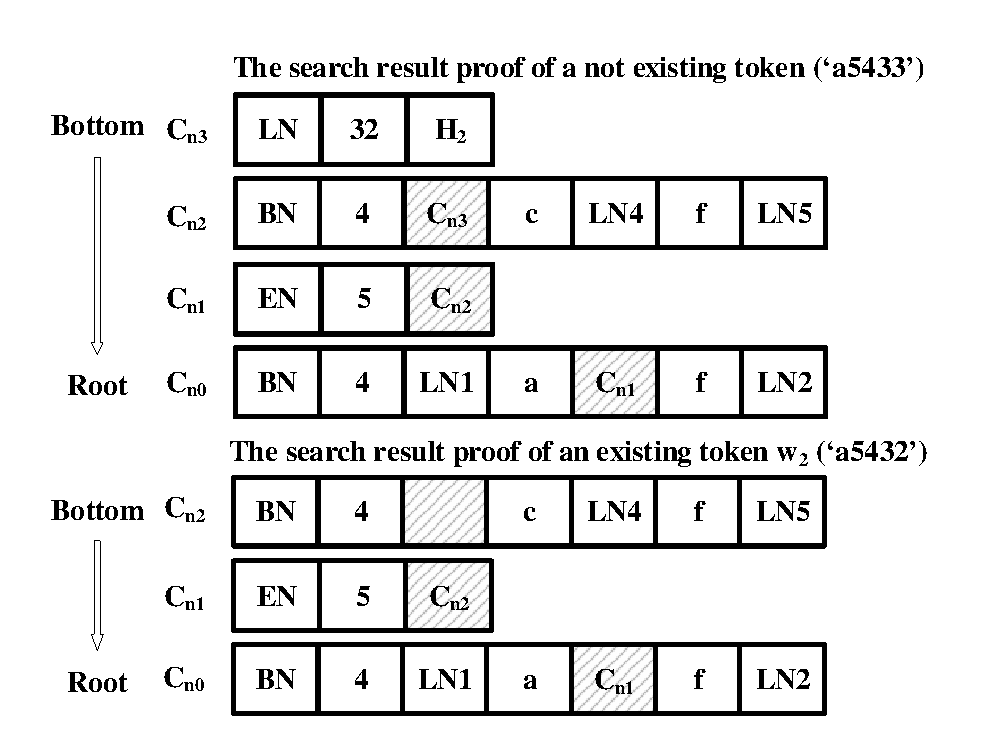
\includegraphics[width= 3.2 in]{fig/resultProof}
    \caption{结果证明}
    \label{fig:resultProof}
  \end{minipage}
\centering
\end{figure}

如图~\ref{fig:inverted-index},图\ref{fig:MPT},图\ref{fig:updateProof}和图\ref{fig:resultProof}所示,我们将通过一个解释性的实例来说明建立和更新验证索引$\lambda$,生成更新证明$\rho_u$和验证更新,以及生成结果证明$\rho_s$和验证搜索结果的过程。

{\heiti 建立并更新验证索引:}首先,我们假设数据持有者拥有四个文件,分别为$d_1,d_2,d_3,d_4$,他们包含了四个关键字$w_1,w_2,w_3,w_4$,其对应关系如图\ref{fig:inverted-index}中的倒排索引所示。由这四个文件构建的验证索引如图\ref{fig:MPT}所示。当包含关键字$w_2$和$w_5$的文件$d_5$新增时,对于已经存在的关键字$w_2$,云服务器只需将$IH(G_{K_2}(d_5))$添加到原有的叶子节点上。而对于不存在的关键字$w_5$,云服务器则需要创建一个新的叶子节点,并将$IH(G_{K_2}(D_5))$作为他的节点值。

{\heiti 生成更新证明和验证更新:}云服务器需要将两个涉及到更新的关键字$w_2$,$w_5$对应的路径返回给用户,用以作为更新证明$\rho_u$。如图~\ref{fig:updateProof}所示,当用户拿到该更新证明后,对于每一个待更新关键字,首先需要确保该关键字对应的令牌或其前缀出现在更新证明中。例如,对于关键字$w_2$,它对应的更新令牌为'a5432',在其更新证明$\sigma_{w_2} = \{C_n3,C_n2,C_n1,C_n0\}$中,我们可以自底向上找到一条路径与该令牌相同。而对于关键字$w_5$,它对应的更新令牌'a5fab'并没有出现在更新证明$\sigma_{w_5} = \{C_n2,C_n1,C_n0\}$中,但他的前缀'a5'出现在了更新证明中,这说明该关键字在验证索引$\lambda$中尚不存在。用户需要首先根据更新证明重构出根节点哈希,用于跟用户持有的根哈希进行对比。只有当每一个待更新关键字对应的更新证明重构出的根哈希与原根哈希相同时,更新验证才通过。验证通过后,用户通过更新令牌$\tau_u$和更新证明$\rho_u$构造出更新后的根哈希$rt'$。对于已存在于$\lambda$中的关键字$w_2$,用户只需要将其对应的哈希值$H_2$更新到$H_2+IH(G_{K_2(d_5)})$,而对于尚不存在于验证索引$\lambda$中的关键字$w_5$,用户需要根据更新证明为其新建叶子节点,即在$C_{n2}$这个分支节点中,添加一个新的分支$f$,使其指向一个新的叶子节点$('ab', IH(G_{K_2(d_5)}))$。最后用户通过联合两个更新证明更新验证索引的根哈希$rt'$,从而确保后续结果验证时的数据新鲜性。

{\heiti 生成结果证明和验证搜索结果:}结果证明$\rho_s$的生成可以分为两种情况来讨论。
第一种情况,假设用户想要搜索的关键字为$w_2$,他提交的对应该关键字的挑战令牌为“a5432”。如图~\ref{fig:resultProof}所示,由于该关键字令牌在验证索引$\lambda$中已经存在,云服务器可以找到与该令牌对应的搜索路径{BN1,EN1,BN2,LN3},根据$Prove$算法,服务器会自底向上返回除$LN3$以外的搜索路径上的“键值对”作为结果证明,如$C_{n2},C_{n1},C_{n0}$所示。用户在收到结果证明$C_{n2},C_{n1},C_{n0}$以后,可以根据该证明$\rho_s$和搜索结果$C_w$重新构建根哈希。具体过程如下:首先用户将令牌“a5432”与结果证明中$\rho_s$的“键”进行匹配,发现“a54”为令牌“a5432”的前缀,因此剩余键$remain\_key$ 为“32”。随后用户根据“32”以及搜索结果$d_2,d_5$重新生成叶子节点$LN3$,并通过结果证明$\rho_s$自底向上构建冲根哈希的值。最后用户通过比较重构得到的根哈希和自身持有的根哈希,来判断数据是否完整。例如,假设云服务器只返回了文件$d_2$,那么重构得到的根哈希将与正确的根哈希不匹配。
第二种情况:假设用户搜索的关键字令牌为“a5433”,该令牌在验证索引$\lambda$中不存在。根据云服务器的查找方法,其搜索路径与“a5432”相同,但不同的是,该令牌在叶子节点$LN3$处发生了不匹配。因此云服务器需要从叶子节点$LN3$开始 (包括$LN3$) 自底向上生成结果证明,如图~\ref{fig:resultProof}中的$C_n3,C_n2,C_n1,C_n0$所示。用户在收到该结果证明以后,由于发现结果证明$\rho_s$中的“键”都不是搜索令牌$\tau_s$的前缀,因此$remain\_key$被置空。用户将直接根据结果证明$\rho_s$重构根哈希。同样,用户将其与正确的根哈希进行对比,如果不相同,则说明服务器篡改了搜索结果或是结果证明,产生了恶意行为。


\section{安全性分析}
\label{sec:single-security}
在本节中,我们将对方案的安全性进行证明。方案的安全性主要分为两个部分,一个是机密性,另一个是可验证性。机密性是指敌手无法从验证索引$\lambda$和用户发送的令牌$\tau$中获取文件和关键字的明文信息。可验证性是指当服务器返回不完整或者不新鲜的结果时,用户不会验证通过。
\begin{figure}[t]
\centering
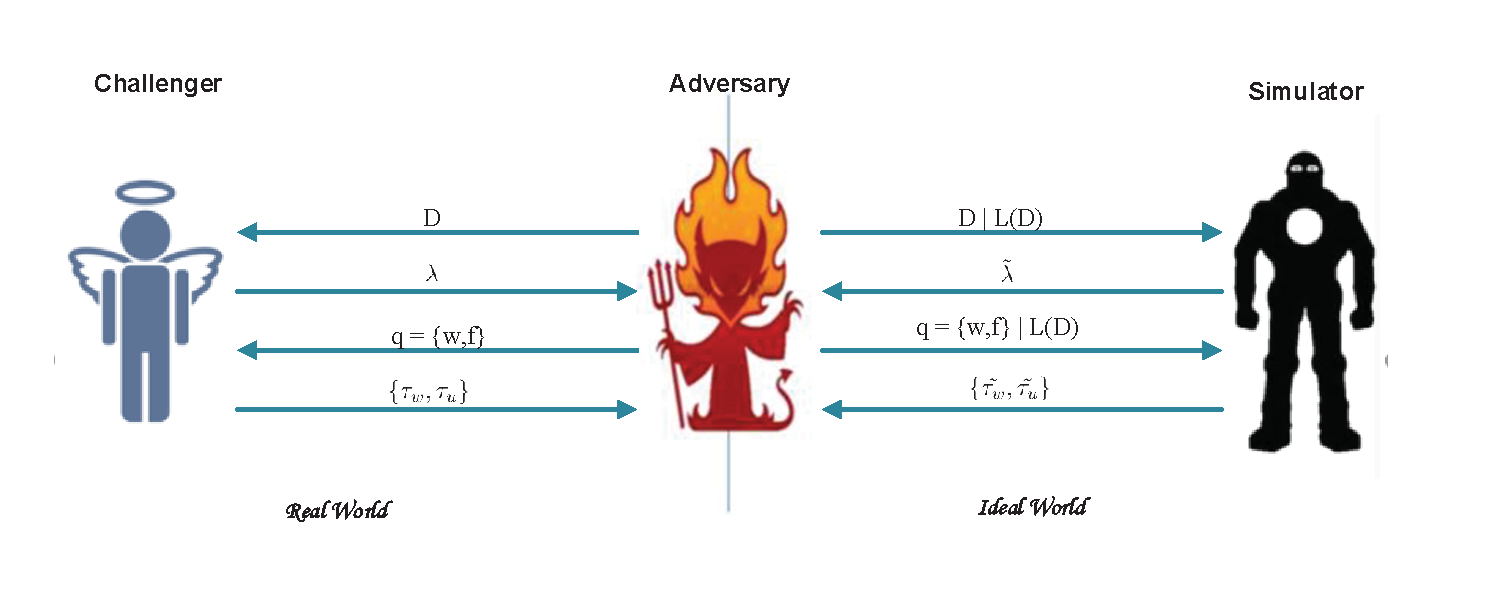
\includegraphics[width=6 in]{fig/security}
\DeclareGraphicsExtensions.
\caption{基于仿真博弈的安全性证明方案}
\label{fig:security}
\end{figure}

首先,我们采用基于仿真博弈 (Simulation-based Game)的安全性方案来证明方案的机密性。该方案的流程解释如图~\ref{fig:security}所示,我们需要确保一个敌手无法区分出$\mathbf{Real}$ World 和$\mathbf{Ideal}$ World 的输出,即公式~\ref{equ:sim}所示。该安全性方案的具体流程如定义~\ref{def:sim}所示:

\begin{definition}[\single 机密性]\label{def:sim}
  {\itshape
      令方案\single 是一个通用的、支持数据更新的可验证对称加密搜索方案,考虑以下概率性实验,其中 $\mathcal{A}$ 是一个有状态的敌手 (statefule adversary), $\mathcal{S}$ 是一个有状态的仿真者 (stateful simulator), $\mathcal{L}$ 是有状态的泄露函数 (leakage algorithms):

      $\mathbf{Real}_\mathcal{A}(k)$:一个挑战者采用$KGen(1^k)$生成了对称秘钥 $K_1,K_2$。敌手 $\mathcal{A}$ 选择了一个文件集 $\mathcal{D}$ 让挑战者通过 $\{\lambda\} \leftarrow Init(K_1,K_2,\mathcal{D})$ 算法生成验证索引 $\lambda$。同时,敌手 $\mathcal{A}$ 生成了多项式数量级的自适应查询 $q = \{w,f\}$。对于每一个查询 $q$, 敌手 $\mathcal{A}$ 从挑战者处收到一个搜索令牌 $\tau_w$ 和 更新令牌 $\tau_u$,其中 $\tau_w \leftarrow SearchToken(K_1,w)$,$(\tau_u) \leftarrow UpdateToken(K_1,K_2,f)$。最后,敌手 $\mathcal{A}$ 返回一个比特 $b$。

      $\mathbf{Ideal}_\mathcal{A,S}(k)$:一个敌手 $\mathcal{A}$ 选择了一个文件集 $\mathcal{D}$。 给定 $\mathcal{L}(\mathcal{D})$,仿真者 $\mathcal{S}$ 生成验证索引 $\lambda$ 发送给敌手 $\mathcal{A}$。敌手 $\mathcal{A}$ 生成了多项式数量级的自适应查询 $q = \{w,f\}$。对于每一个查询 $q$,仿真者 $\mathcal{S}$ 向其返回一个恰当的令牌 $\tau$。最后,敌手 $\mathcal{A}$ 返回一个比特 $b$。

      如果对于任何概率多项式时间 (Probabilistic Polynomial-Time, PPT)的敌手 $\mathcal{A}$, 始终存在一个概率多项式时间的仿真者 $\mathcal{S}$,使得,
      \begin{align}
        \label{equ:sim}
        |Pr[\mathbf{Real}_A(k) = 1] - Pr[\mathbf{Ideal}_{A,S}(k) = 1]| \leq negl(k).
      \end{align}
      则我们认为 \single 是 $\mathcal{L}$-机密的。
  }
\end{definition}


在具体证明之前,我们首先给出敌手$\mathcal{A}$能看到的内容,即泄露函数$\mathcal{L}$的内容,如公式~\ref{equ:leakage}所示:

\begin{align}\label{equ:leakage}
  \mathcal{L}(\mathcal{D})=(|\lambda|,{\tau}_q,{\sigma})
\end{align}

其中$|\lambda|$表示验证索引的大小,以叶子节点的数目来衡量。$\{\tau_q\}$表示由$q$个查询产生的令牌,$\sigma$表示验证索引中的搜索路径,则我们有定理~\ref{theo:sim}:

\begin{theorem}\label{theo:sim}
    如果$F$,$G$都是伪随机函数,那么方案\single 就是$\mathcal{L}$-机密的。
\end{theorem}

\begin{proof}
  我们将证明,对于任何概率多项式时间内的敌手$\mathcal{A}$,都存在一个概率多项式时间内的仿真者$\mathcal{S}$,使得真实游戏 $\mathbf{Real}_\mathcal{A}(k)$和仿真游戏 $\mathbf{Ideal}_\mathcal{A,S}(k)$在计算上是无法区分的 (Computationally Indistinguishable),而在现代密码学中,不可区分性等同于机密性。

  首先,给定$\mathcal{L}(\mathcal{D})=(|\lambda|,{\tau}_q,{\sigma})$,$\mathcal{S}$通过选择$|\lambda|$个随机“键值对”插入MPT中生成一个仿真的验证索引$\tilde{\lambda}$。由于在真实的验证索引中,“键值对”都是采用了伪随机函数$F$,$G$进行了伪随机化的,因此敌手$\mathcal{A}$将无法区分出真实的$\lambda$和仿真的$\tilde{\lambda}$。

  模拟搜索令牌时,对于挑战者生成的第一个令牌 $\tau_w$ ,如果它与 $\{\sigma\}$ 中的某一路径匹配,那么仿真者 $\mathcal{S}$ 就在 $\tilde{\lambda}$ 中选择任意一条路径作为令牌 $\tilde{\tau_w}$ 发送给敌手 $\mathcal{A}$,否则 $\mathcal{S}$ 就选择不在 $\tilde{\lambda}$ ̃路径中的随机字符串作为令牌 $\tilde{\tau_w}$ 发送给敌手 $\mathcal{A}$。对于后续的令牌,如果 $\tau_w$ 之前出现过,那么令牌 $\tilde{\tau_w}$ ̃就和之前发送给敌手 $\mathcal{A}$的维持一样。如果 $\tau_w$ 没出现过,那么令牌的生成方式就和第一个令牌的生成方式一样。由于令牌采用了伪随机函数$F$进行了加密,因此敌手$\mathcal{A}$也无法区分真实的令牌和仿真的令牌。

  模拟更新令牌时,更新令牌被设置为$\tilde{\tau_u} = (\tilde{\tau_{w_1}},\cdots,\tilde{\tau_{w_{|W_d|}}},\tilde{\tau_d})$。对每一个更新令牌$\tilde{\tau_{w_i}}$,其中$i \in \{1,\cdots, |W_d|\}$,$\mathcal{S}$ 的模拟方法与模拟搜索令牌方法相同。由于每一个更新令牌都采用了伪随机函数$F$进行了加密,并且文件$d$采用了伪随机函数$G$进行了加密,因此敌手 $\mathcal{A}$ 无法区分真实的令牌、文件与仿真的令牌、文件。

  因此我们可以得到结论:真实实验$\mathbf{Real}_\mathcal{A}(k)$和仿真实验$\mathbf{Ideal}_\mathcal{A,S}(k)$的输出结果是不可区分的。
\end{proof}

\single 方案的可验证性意味着该方案可以验证数据的新鲜性和完整性,即防御定义~\ref{def:freshness}和~\ref{def:integrity}提出的两种攻击。这里我们采用了一个基于游戏 (game-based)的安全性定义来证明\single 方案的可验证性,该定义表明,敌手提供伪造的搜索结果,而用户验证通过的概率是小于一个可忽略的数的,如公式~\ref{equ:game}所示,其具体定义如~\ref{def:game}所示:

\begin{definition}[\single 可验证性]\label{def:game}
  \itshape{
      令方案\single 是一个通用的、支持数据更新的可验证对称加密搜索方案,考虑以下概率性实验,其中 $\mathcal{A}$ 是一个有状态的敌手:

      \noindent$\mathbf{Vrf}_\mathcal{A}(k)$:
      \begin{enumerate}[1.]
        \item 挑战者通过 $KGen(1^k)$ 生成对称秘钥 $K_1,K_2$。
        \item 敌手 $\mathcal{A}$ 给挑战者选择一个文件集合 $\mathcal{D}$。
        \item 挑战者通过$\{\lambda\} \leftarrow Init(K_1,K_2,\mathcal{D})$生成一个验证索引 $\lambda$。
        \item 给定 $\lambda$ 和 对算法 $SearchToken(K_1,w)$, $UpdateToken(K_1,K_2,d)$ 的预言权限, 敌手 $\mathcal{A}$ 选择一个关键字令牌 $\tau_w$, 和一系列加密文件 $\tilde{C_w}$,其中 $\tilde{C_w} \neq C_w$,同时输出%更新证明 $\rho_u'$ 和
        结果证明$\tilde{rho_s}$.
        \item 挑战者计算 $b:=Verify(K_1,K_2,\tilde{C_w},\tilde{rho_s},\tau_w)$.
        \item 实验的输出为一个比特 $b$.
      \end{enumerate}
      如果对于任何概率多项式时间 (Probabilistic Polynomial-Time, PPT)的敌手 $\mathcal{A}$,
      \begin{align}\label{equ:game}
        Pr[\mathbf{Vrf}_\mathcal{A}(k)=1] \leq negl(k).
      \end{align}
      成立,则我们认为\single 方案是可验证的。
  }
\end{definition}

根据定义~\ref{def:game},我们有定理~\ref{theo:game}:
\begin{theorem}\label{theo:game}
    如果哈希函数$H$和增量哈希函数$IH$是抗碰撞的,并且$G$是伪随机函数,那么\single 方案就是可验证的。
\end{theorem}

\begin{proof}
  考虑服务器返回的搜索结果为$\tilde{C_w}$,而正确的搜索结果为$C_w$,其中$\tilde{C_w} \neq C_w$。但是用户的$Verify$算法通过了$\tilde{C_w}$作为正确搜索结果的情况。对于$Verify$算法,这种情况的产生存在两种可能。第一种可能是在计算$\tilde{C_w}$ ̃和$C_w$对应的伪随机值$G_{K_2}(d)$时产生了碰撞,其中$d \in D_w$, $D_w$为$C_w$的明文信息,或者是在计算对应的增量哈希值$\sum_{d \in D_{w}}IH (G_{K_2} (d))$时产生了碰撞。第二种是在生成根哈希的路径中产生了哈希碰撞。不管是哪一种,都可以推出哈希函数产生了碰撞或者伪随机函数产生了碰撞,但是哈希函数产生碰撞或者伪随机函数产生碰撞的可能性是小于一个可忽略的值的,因此,我们的方案是可验证的。
\end{proof}


\section{性能评价}



\subsection{实验设置}
为了证明方案\single 的有效性,我们通过 Crypto++ 5.6.5 库实现了方案的原型。原型系统包含大约2200行代码。我们使用 HMAC-SHA256 作为两个随机预言 (random-oracle),使用 SHA3-256 作为哈希函数,使用 MuHash 作为增量哈希函数。我们的实验在一台处理器为 Intel Core i5 2.5GHz,内存为 4G 的笔记本上进行,使用单线程实现。

我们使用一个开源数据集Enron email dataset~\cite{enronemail}作为实验的测试数据集,使用了其中从“allen-p”到“kaminski-v”之间的数据。我们从该数据集中提取出了大量的“文件-关键字”对 (document-keyword pairs),并通过python脚本为他们构建出了明文的倒排索引。注意,从文件中提取关键字的时延并没有被考虑在实验评估中,因为该问题与我们研究的\single 方案是一个独立的问题。

下文中,我们首先评估了\single 方案的算法效率,然后将\single 方案与一个著名的对称加密搜索方案~\cite{cash2014dynamic}进行了结合,以此来证明\single 方案引入的结果验证的开销并不大。注意,如无特别说明,下文中的每一个实验结果都是十次实验的平均值。


\subsection{实验结果}

首先,我们评估了$Init$算法的时延,即数据持有者生成验证索引$\lambda$所需的时间。$Init$算法需要数据持有者对每一个“文件-关键字”对生成键值对,其中“键”为关键字的伪随机值,“值”为包含该关键字的所有文件的增量哈希和。如图~\ref{fig:init}所示,由于验证索引$\lambda$的生成需要对每一个“文件-关键字”操作,即加密后向MPT中执行的插入操作,因此其所需时间与“文件-关键字”对的数量大小成正比。总体来说,$Init$ 算法在 “文件-关键字”对达到400万的时候,可以在25秒内执行完毕。由于$Init$算法仅需要在数据持有者在初始化时执行一次,因此这个开销是可以接受的。
\begin{figure}[h]
\centering
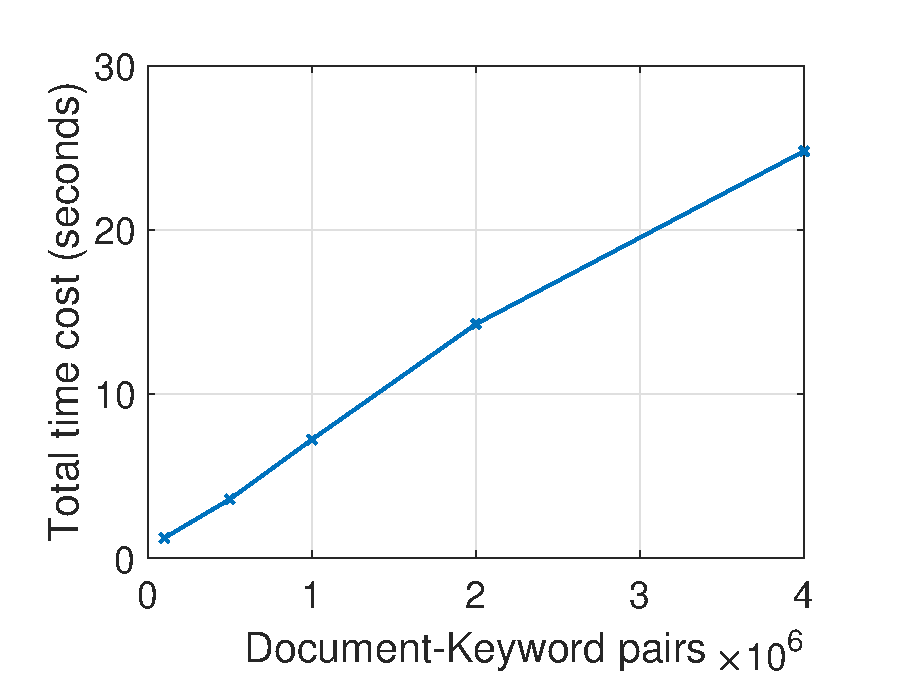
\includegraphics[width=3.5 in]{expr/initialization}
\DeclareGraphicsExtensions.
\caption{$Init$ 算法的开销}
\label{fig:init}
\end{figure}
%The delays of generating the proof index are proportional to the size of the document-keyword pairs, since \name performs the same number of insertions to the number of the document-keyword pairs. Overall, the initialization consumes around 25 seconds where the documents include four million keywords, which is acceptable.
% for the initialization process.

云服务器更新验证索引的时间如图~\ref{fig:update}所示,更新算法$Update$的时延与数据库的大小有关,即与验证索引的大小有关,而验证索引的大小由它包含的关键字数量来衡量。严格意义上来说,一次更新的时延与MPT树的层数有关。为了更好的展示更新时延与验证索引大小的关系,我们使用了不同大小的数据库大小来评估更新时延。由于每一个文件包含的关键字个数不同,这里我们采用吞吐量(throughput)来衡量每秒钟云服务器可以更新的“文件-关键字”对。需要注意的是,$Update$操作包括$Add$和$Del$两种操作,每一个关键字的更新不仅需要服务器更新相应的叶子节点,还需要服务器返回相应的搜索路径作为更新证明。从图中可以看到,$Add$和$Del$操作的性能几乎相同。当数据库的大小增大时,吞吐量将会降低。当数据库的大小为100万个关键字时,云服务器每秒钟可以同时支持30,000次更新操作。同时,我们也测量了用户端$UpdateToken$算法引入的带宽开销,更新令牌$\tau_u$中每一个关键字对应的密文带来的平均开销大小在 32字节左右,而更新令牌的总大小与待更新文件$d$包含的关键字个数有关。
\begin{figure}[h]
\centering
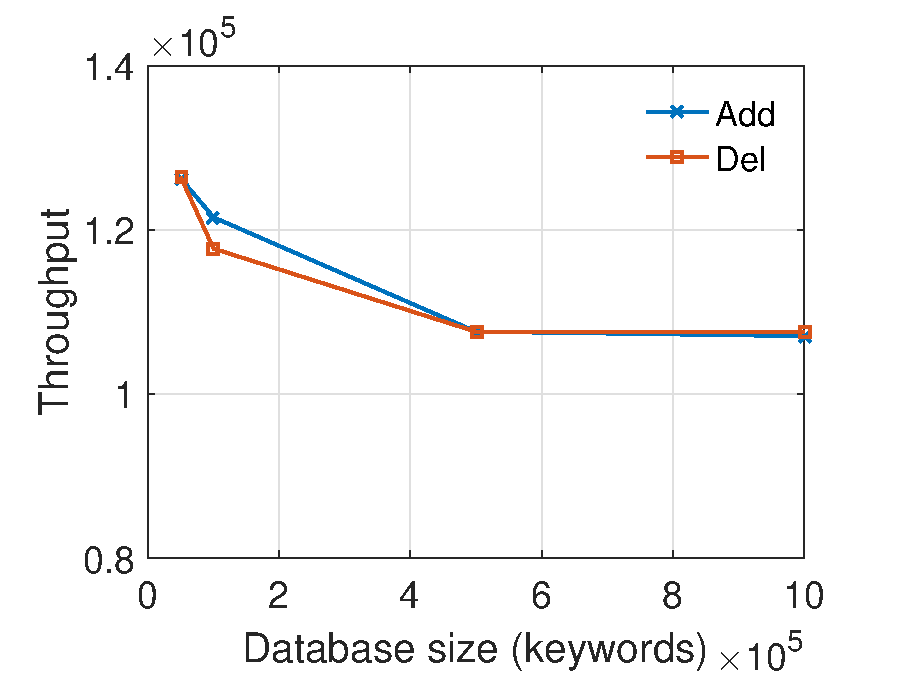
\includegraphics[width=3.5 in]{expr/update}
\DeclareGraphicsExtensions.
\caption{$Update$ 算法的吞吐量}
\label{fig:update}
\end{figure}



更新验证算法$VerifyUpdate$的执行时间与用户更新文件所包含的关键字个数相关,因此我们采用了单个关键字更新验证需要的平均时间来进行评估。注意,数据持有者验证更新的操作包括对每一个更新令牌生成根哈希进行比对,当所有的更新令牌都验证通过后,最后在进行根哈希的生成。这里,我们只评估了验证每一个根哈希所需要的开销,因为相对生成更新后的根哈希,验证每一个更新令牌是否准确是该算法的主要开销。我们采用了数据库大小分别为5万,10万,50万和100万来衡量数据持有者验证更新证明的时间开销。 如图~\ref{fig:verifyupdate}所示,数据持有者验证每一个搜索令牌的开销随着数据库的增大而逐渐增长,并且逐渐趋于平缓。当数据库的大小为50万个关键字时,一个关键字的更新验证操作平均需要55微秒的时间。即,在验证索引包含50万个关键字时,数据持有者更新一个包含1千个关键字的文件,也只需要55毫秒的时间。
\begin{figure}[h]
\centering
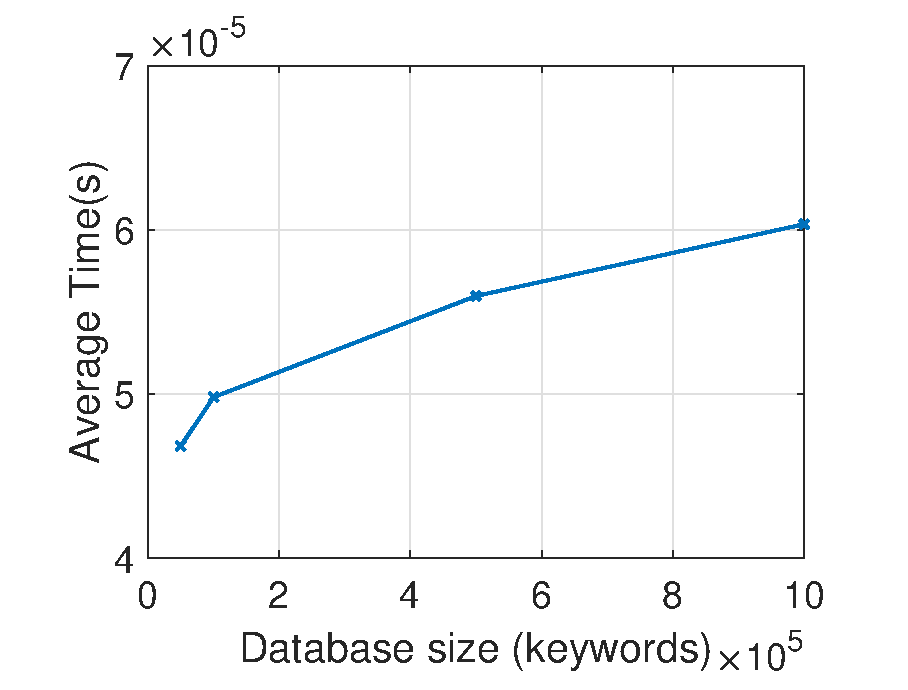
\includegraphics[width=3.5 in]{expr/verifyupdate}
\DeclareGraphicsExtensions.
\caption{$VerifyUpdate$ 算法的开销}
\label{fig:verifyupdate}
\end{figure}


$Prove$算法由云服务器执行,在数据持有者提交搜索请求时,云服务器需要根据搜索令牌在验证索引中查找到该关键字,并将其搜索路径作为结果证明返回。图~\ref{fig:prove}中显示了该算法的开销,包括计算开销和通信开销。其中红色的线表示云服务器执行$Prove$算法的计算开销,而蓝色的线表示云服务器生成的结果证明的大小,即通信开销。从图中可以看到,云服务器可以在数据库大小在100万关键字时,每秒钟进行43,000次 $Prove$ 操作,这意味着云服务器可以同时支持43,000个来自用户的查询请求。由$Prove$操作产生的结果证明$\rho_s$的大小也可以在图中看到,结果证明的大小随着数据库的增长而逐渐增长,趋于平缓。但总体而言,当数据库的大小在100万关键字时,结果证明的大小也只需要2.5KB左右。
\begin{figure}[h]
\centering
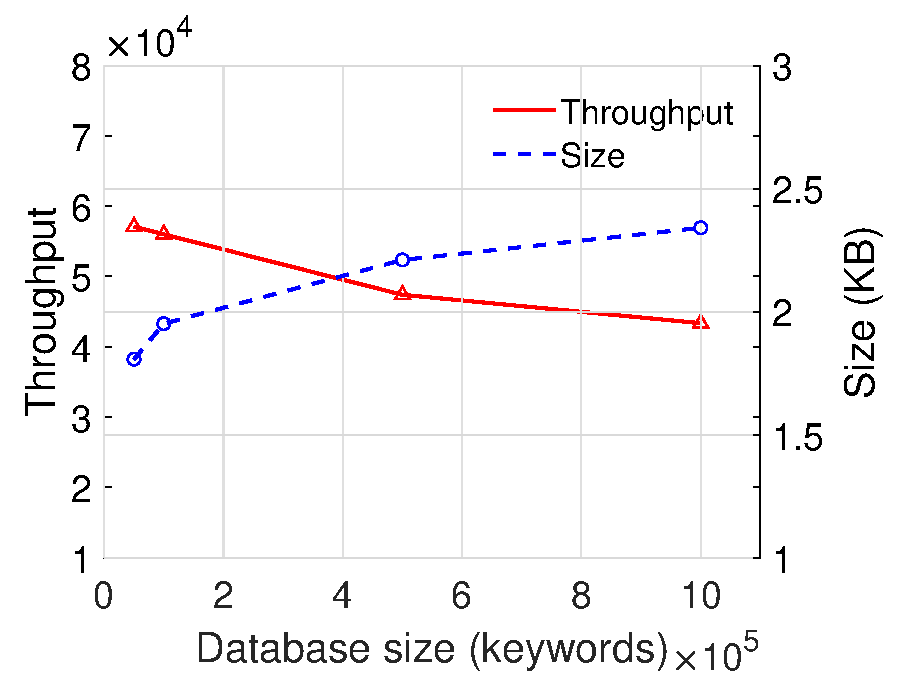
\includegraphics[width=3.5 in]{expr/prove}
\DeclareGraphicsExtensions.
\caption{$Prove$ 算法的吞吐量}
\label{fig:prove}
\end{figure}

$Verify$算法由数据持有者执行,数据持有者在收到云服务器返回的搜索结果和结果证明以后,需要重构出根哈希,并通过与自身保留的根哈希进行对比来确保搜索结果完整性。这里,我们通过累计分布函数图 (Cumulative Distribution Function, CDF)来对用户端进行的$Verify$算法进行测试。这里采用的数据库大小为10万个关键字,即在验证索引大小为10万个关键字的情况下,数据持有者最快可以在0.05毫秒内完成验证操作,最长需要0.1毫秒以上的时间。总体来说,该算法需要的验证时间分布较为集中,在99.7\%的概率下,数据持有者可以在0.1毫秒内完成结果验证,如图~\ref{fig:verify}所示。对于一个非频繁搜索的数据持有者来说,0.1毫秒的时间是完全可以接受的。
\begin{figure}[h]
\centering
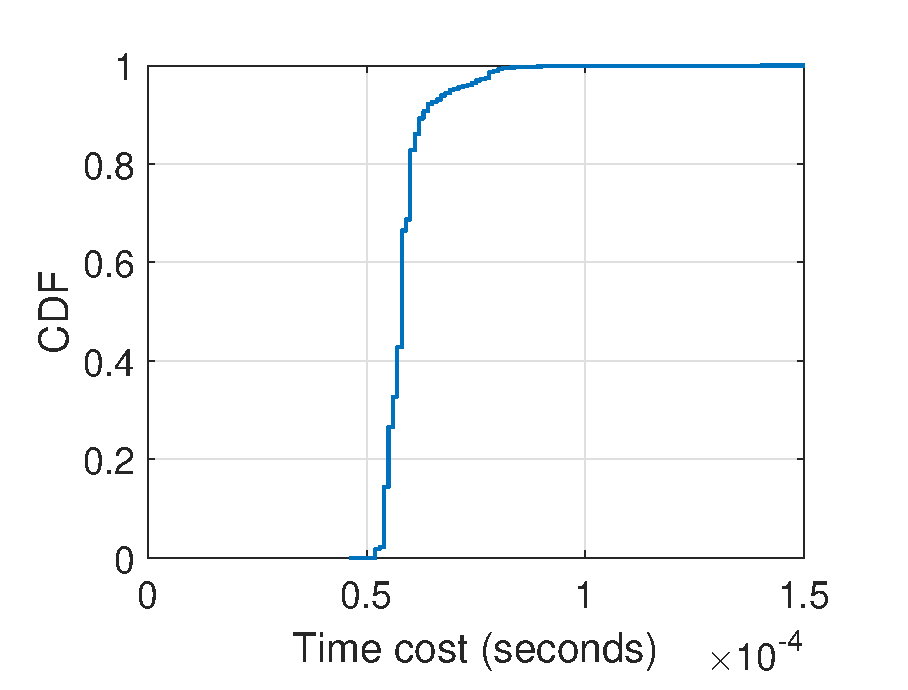
\includegraphics[width=3.5 in]{expr/verify}
\DeclareGraphicsExtensions.
\caption{$Verify$ 算法的开销}
\label{fig:verify}
\end{figure}

除了计算开销以外,我们还对算法引入的通信开销进行了评估,即由$Update$算法和$Prove$算法引入的更新证明和结果证明的开销。需要注意的是,由于更新证明和结果证明本质上都是搜索令牌在验证索引上的搜索路径,因此其大小与验证索引的层数直接相关,即与MPT的层数相关。如图~\ref{fig:proof}所示,这里我们将MPT的层数作为参数来对其进行了衡量。另外,由于更新证明和结果证明的结构相同,因此我们采用了一个实验来衡量单个关键字产生的更新证明(结果证明)的通信开销。从图中可以看到,随着关键字个数的增长,结果证明(更新证明)的开销呈现对数形式增长。这是因为当验证索引达到10层时,并不是每一个“文件-关键字”对都存储于验证索引的第10层,而是根据关键字令牌的分布情况,散落在验证索引的各个层次。因此虽然验证索引的层数逐渐增长,但平均情况下,每一个关键字令牌产生的更新证明(结果证明)增长较为缓慢。从图中可以看到,一个关键字带来的平均更新证明开销为2.5KB左右,即如果用户更新的文件包含1千个关键字,那么更新证明的开销就为2.5MB左右。而对于结果证明,由于每次用户只搜索一个关键字,因此结果证明的开销即为2.5KB。

\begin{figure}[h]
\centering
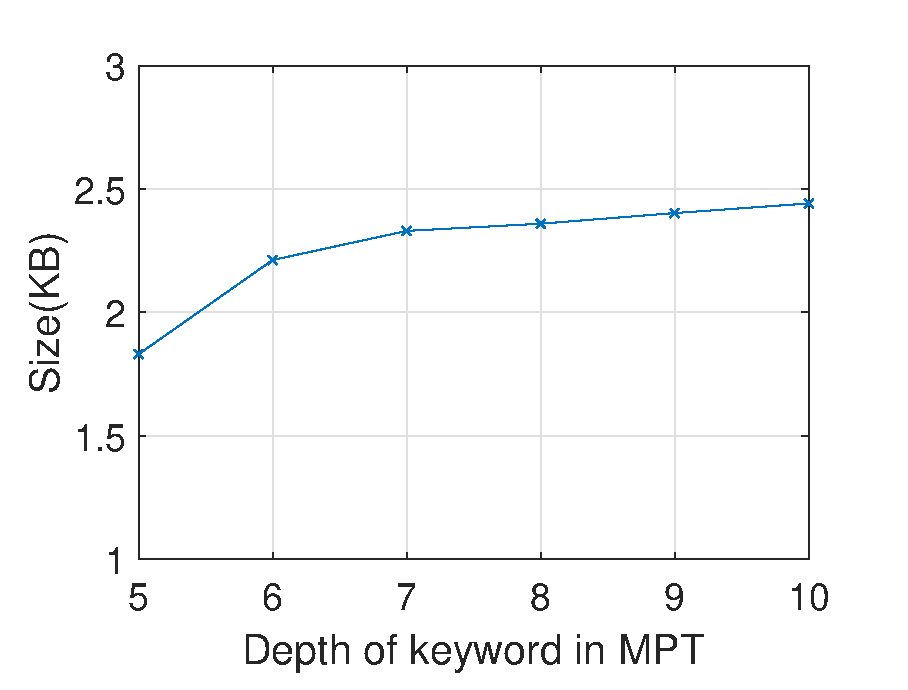
\includegraphics[width=3.5 in]{expr/proof}
\DeclareGraphicsExtensions.
\caption{更新证明和结果证明的通信开销}
\label{fig:proof}
\end{figure}


除此以外,我们还对基于MPT构建的验证索引的的存储空间进行了评估。由$Init$算法可知,存储在MPT中的数据为每一个“文件-关键字”对的加密形式,其中“键”为每一个关键字的伪随机值,而“值”为包含该关键字的所有文件的增量哈希和。如图~\ref{fig:storage}所示,如果我们使用一个100万个关键字的数据库,验证索引的存储空间大小大约为82MB,而该数据库本身所占用的空间大小为 590MB,相对而言,基于MPT构建的验证索引带来的额外存储开销不算特别大。特别需要说明的是,这里我们评估验证索引的大小所采用数据集为关键字密集型的数据,即邮件数据。如果数据持有者需要加密的是媒体类型的数据,例如图片或是音乐文件等等,这些文件只包含少量的关键字和属性,因此为这些类型的数据构建验证索引时,验证索引占原数据集的比例将会很小,甚至可以忽略。

\begin{figure}[h]
\centering
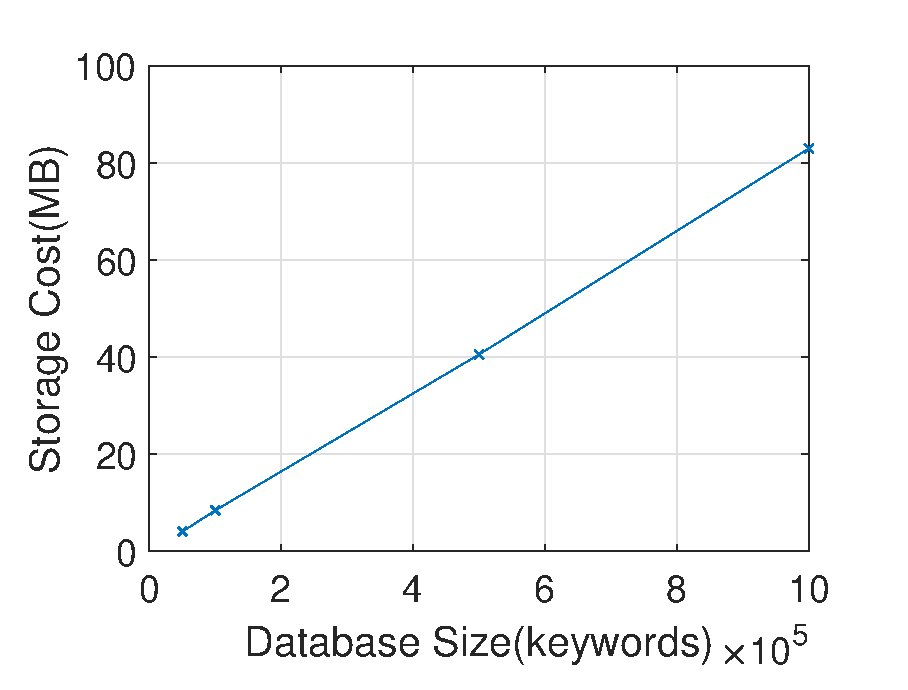
\includegraphics[width=3.5 in]{expr/storage}
\DeclareGraphicsExtensions.
\caption{验证索引$\lambda$的存储开销 }
\label{fig:storage}
\end{figure}

\subsection{与SSE方案的对比}
我们将我们的通用可验证对称加密搜索方案\single ,与Cash等人提出的一个较为知名的动态对称加密搜索方案 (Dynamic Symmetric Searchable Encryption, DSSE)~\cite{cash2014dynamic}进行了结合,并展示了\single 为其提供结果验证服务带来的额外开销,如图~\ref{fig:comparison}所示。
\begin{figure}[h]
\centering
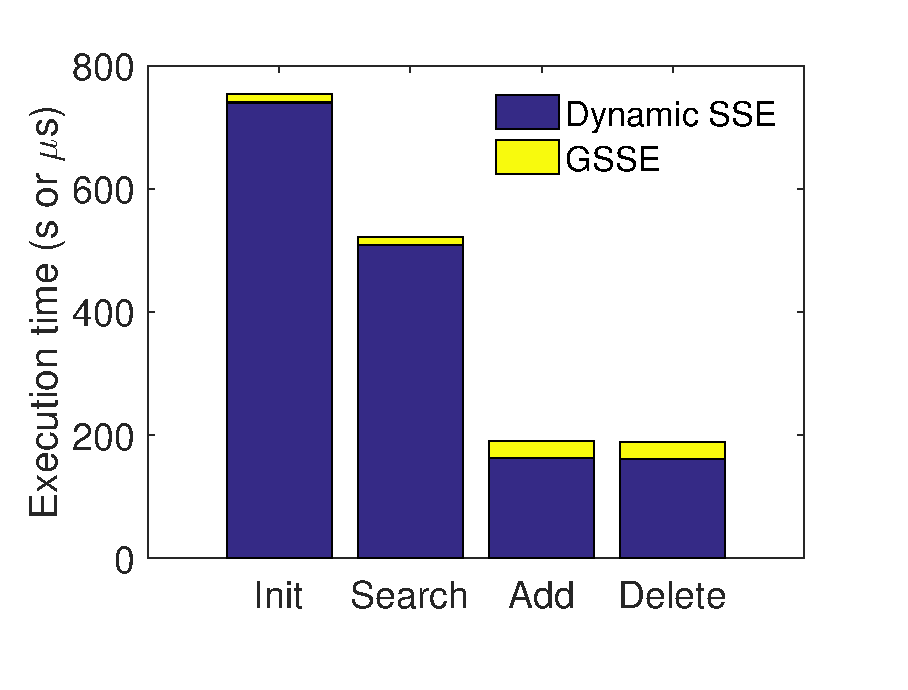
\includegraphics[width=3.5 in]{expr/comparison}
\DeclareGraphicsExtensions.
\caption{与DSSE方案~\cite{cash2014dynamic}的对比}
\label{fig:comparison}
\end{figure}
为了公平的进行性能比较,我们使用了同样的数据集,并在同样的设备参数下对两个方案联合进行了实验。如图~\ref{fig:comparison}所示,我们测量了$Init$阶段,$Search(Prove)$阶段和$Update$阶段的性能开销。图中,$Init$操作使用了200万个“文件-关键字”来分别构建DSSE方案~\cite{cash2014dynamic}和方案\single 用到的索引,时间单位为秒。而其他三个操作$Search(Prove), Add, Delete$的评估采用的数据库大小为10,000个关键字,时间单位为微秒。注意,DSSE方案中的$Search$操作与\single 方案中的$Prove$操作对应。从图中可以看出,我们的\single 方案引入的额外开销非常小。其中,相较于DSSE方案而言,方案\single 在$Init$阶段引入的开销非常小,仅仅额外引入了1.9\%的额外开销。而对于一次$Search(Prove)$ 操作来说,\single 方案给云服务器引入的额外开销为14微秒,仅仅给DSSE方案带来了2\%的额外开销。同样的,对于一次$Add$或$Delete$操作来说,我们的\single 方案仅仅引入了27微秒的时间,仅占方案~\cite{cash2014dynamic}的 17\%。

在表~\ref{tab:compareSSE}中,我们还比较了二者的通信开销。由于数据的方差较大,每一个实验结果都是50,000次实验的平均值。

\begin{table}[h]
  \begin{center}
  \caption{与DSSE方案~\cite{cash2014dynamic}结合后的通信开销对比}
  \label{tab:compareSSE}
  %\begin{threeparttable}
  \begin{tabular}{c c c c}
    \hline
    通信开销    & DSSE~\cite{cash2014dynamic} &\single       &  占比 \\
    \hline
    搜索令牌          & 390 B                 & 32 B         & 8.2\%\\

    搜索结果/结果证明   & 53 KB              & 3 KB         & 5.7\%\\
    \hline
  \end{tabular}
\end{center}
\end{table}
\vspace{-0.075in}
结果显示,DSSE方案的搜索结果大小平均为53KB左右,而我们的结果证明大小仅仅为3KB左右,即由\single 方案引入的额外开销低于6\%。此外,DSSE方案~\cite{cash2014dynamic}生成的令牌大小平均为390B,而\single 方案生成的令牌仅为32B,即由\single 方案引入的额外开销低于9\%。这些实验结果充分表明了,\single 方案是实用且高效的。



\section{本章总结}
本章从定义、算法,安全性分析和实验几个角度,对\single 方案进行了充分的研究与分析。\single 方案为用户在不可信云存储环境下提供了加密搜索解决方案,即为传统加密搜索方案提供了结果验证功能。总体来说,\single 方案完成了以下几点主要贡献。
\begin{itemize}
  \item 功能完善:\single 方案同时解决了数据新鲜性和数据完整性的验证。特别地,对于不可信云服务器故意返回空结果来规避结果验证的情况,\single 也提出了解决方案,并且不需要用户在本地维护关键字集合。该问题是一个严重的安全漏洞,但现有的许多工作都忽略了该问题。\single 方案首次对该问题进行了强调并进行了解决;
  \item 安全性:传统加密搜索方案以云服务器半可信为前提来提出解决方案,而\single 方案以云服务器不可信为前提。这种更真实的前提假定使\single 方案可以面对一个更强的敌手,因此也使得基于该假定设计的\single 方案具有更强的安全性;
  \item 高效性:\single 方案的高效性体现在两个方面,一方面\single 方案的算法操作可与加密搜索方案的算法操作并行执行,在与加密搜索方案解耦的前提下,又在流程上与其紧密结合,提升了整体的执行效率。另一方面,从与加密搜索方案的对比实验中可以看出,\single 方案的效率很高,每一步操作给整体方案带来的额外开销很小,并且\single 方案执行结果验证的效率也很高,几乎可以忽略不计;
  \item 通用性:\single 方案通过索引解耦,将结果验证功能从加密搜索方案中独立出来,使得\single 方案可以为任何加密搜索方案提供结果验证功能,包括对称加密搜索方案甚至是公钥加密搜索方案。
\end{itemize}

\chapter{多用户下的可验证对称加密搜索方案研究}
\label{cha:multi-user}
\section{引言}
本章在\single 的基础上,提出了一种适用于多用户场景下的可验证对称加密搜索方案\multi 。该方案同样可以与任意多用户场景下的加密搜索方案结合,来为其提供结果验证功能。与\single 方案不同的是,在多用户的场景下,即数据共享的情况下,数据持有者与数据搜索者产生了分离。数据持有者一方面需要对数据搜索者进行访问控制,以确保数据搜索者只能读取数据而无法写入数据。另一方面,为了保证数据新鲜性,数据持有者还需要在数据发生了更新时,告知数据搜索者。我们将通过公私钥机制解决访问控制问题,并通过时间戳链机制解决数据新鲜性问题。本章的主要内容安排如下:首先介绍了多用户场景下的系统框架,明确了该框架的参与方及所承担的计算任务;随后通过一个抽象定义对该方案工作的流程进行了说明;算法分析部分对抽象定义中的具体算法进行了详细分析;最后,通过安全性分析和实验结果验证了本方案的安全性和有效性。



\section{系统架构}

\begin{figure}[t]
\centering
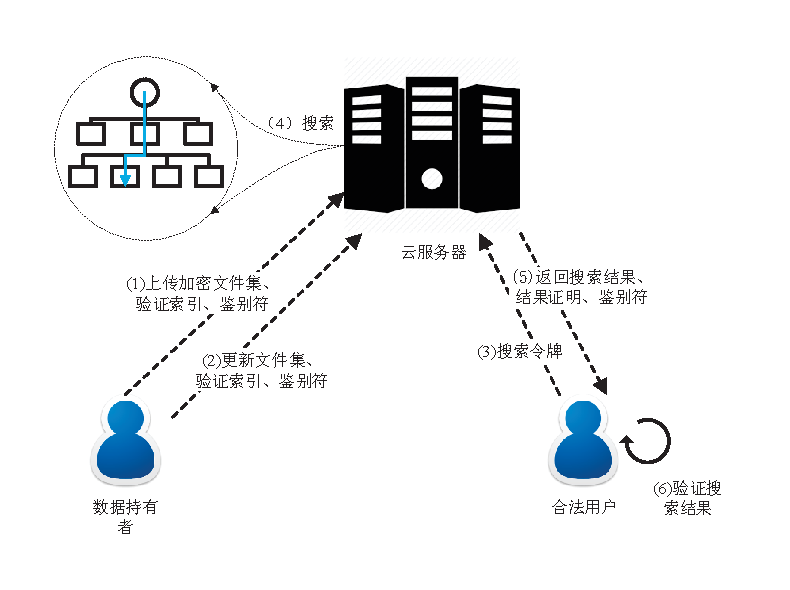
\includegraphics[width=6 in]{fig/GM-VSSE}
\DeclareGraphicsExtensions.
\caption{多用户场景下的可验证对称加密搜索框架\multi}
\label{fig:GM-VSSE}
\end{figure}

多用户场景下的可验证对称加密搜索方案\multi 如图~\ref{fig:GM-VSSE}所示,数据持有者和数据搜索用户产生了分离。首先数据持有者仍然需要对文件集进行处理,得到加密文件集和验证索引,同时他还需要生成一个鉴别符,将三者上传给云服务器。数据持有者在有需要的时候,也需要更新其文件集、验证索引和鉴别符。当一个数据搜索用户被数据持有者授权进行搜索时,他成为了一个合法用户。他可以通过提交搜索令牌来对数据持有者的加密文件集进行搜索。云服务器在收到该搜索令牌以后,需要向其返回加密搜索结果,结果证明以及鉴别符。通过这种方式,我们使得合法用户可以按需获取搜索结果并进行结果验证。


\section{方案流程}
在描述\multi 方案的工作流程前,我们先回顾多用户对称加密搜索方案的常见定义。
\begin{definition}[\textbf{MSSE 方案}]\label{def:MSSE}
  {\itshape
      一个支持文件更新的$MSSE$ 方案,参与方有三个, 分别为数据持有者,合法用户以及半可信的云服务器。数据持有者向云服务器提供提供加密数据集和搜索索引,同时数据持有者可以对合法用户进行注册和撤销。云服务器可以为合法用户提供搜索功能。一个$MSSE$方案是以下八个算法的集合:
      \begin{itemize}
        \item $KGen_{\mathcal{MSSE}}(1^k) \rightarrow \{\mathcal{K},K_O\}$: 是由数据持有者执行的秘钥生成算法。它将一个安全参数作为输入,输出一系列对称秘钥$\mathcal{K}$和一个用户私钥$K_O$。
        \item $EnrollUser_{\mathcal{MSSE}}(K_O,U) \rightarrow \{K_U\}$: 是由数据持有者执行的用户注册算法。它将数据持有者的私钥 $K_O$ 和待注册用户的身份证明 $U$作为输入, 输出该用户的私钥$K_U$。数据持有者将私钥$K_U$ 发送给用户$U$. 该算法将一个用户添加到了数据持有者的合法用户集合中,即授权该用户对数据持有者的数据进行搜索。
        \item $RevokeUser_{\mathcal{MSSE}}(K_O,U) \rightarrow \{b\}$ : 是由数据持有者执行的用户撤销算法。它将数据持有者的私钥 $K_O$ 和待注册用户的身份证明 $U$, 输出一个比特$b$。如果$b=1$表示撤销成功,反之。该算法将一个用户从数据持有者的合法用户集中移除,即取消该用户对数据持有者数据的搜索权限。
        \item $Init_{\mathcal{MSSE}}(\mathcal{K}, \mathcal{D}) \rightarrow \{\gamma, \mathcal{C}\}$: 是由数据持有者执行的初始化算法。它将对称秘钥$\mathcal{K}$和明文文件集$\mathcal{D}$作为输入,输出搜索索引$\gamma$和密文文件集$\mathcal{C}$。数据持有者将搜索索引$\gamma$和密文文件集$\mathcal{C}$上传给云服务器。
        \item $UpdateToken_{\mathcal{MSSE}}(\mathcal{K}, d) \rightarrow \{\tau_u\}$: 是由数据持有者执行的更新令牌生成算法。它将对称秘钥$\mathcal{K}$和需要更新的文件$d$作为输入,输出一系列更新令牌$\tau_u$。数据持有者将更新令牌$\tau_u$上传给云服务器。
        \item $Update_{\mathcal{MSSE}}(\gamma, \tau_u) \rightarrow \{\gamma'\}$: 是由云服务器执行的更新算法。它将搜索索引$\gamma$和更新令牌$\tau_u$作为输入,输出更新后的搜索索引$\gamma'$。
        \item $SearchToken_{\mathcal{SSE}}(\mathcal{K}, w) \rightarrow \{\tau_{w}\}$: 是由合法用户执行的搜索令牌生成算法。它将对称秘钥$\mathcal{K}$和某一关键字$w$作为输入,输出与该关键字相关搜索令牌$\tau_{w}$。合法用户将该搜索令牌 $\tau_{w}$上传给云服务器进行搜索。
        \item $Search_{\mathcal{MSSE}}(\gamma, \tau_{w}) \rightarrow \{C_w\}$: 是由云服务器执行的搜索算法。它将搜索索引$\gamma$和搜索令牌$\tau_{w}$作为输入,输出搜索结果$C_w$。云服务器将搜索结果$C_w$返回给合法用户。
      \end{itemize}
      }
\end{definition}

注意,这里需要说明的是,本方案的目的不是设计多用户的对称加密搜索方案,而是为了给这些已有的方案提供结果验证功能。本方案在\single 的基础上进行了改进,验证索引的构建仍然需要利用默克尔帕特里夏树和增量哈希技术,同时\multi 方案还使用了时间戳链和公私钥加密体系来实现跨用户的数据新鲜性和数据完整性验证。\multi 方案的具体定义如下。

\begin{definition}[\textbf{\multi 方案}]\label{def:multi}
  {\itshape
      在 \multi 方案中,参与方有三个, 分别为数据持有者,合法用户以及不可信的云服务器。数据持有者向云服务器提供一个验证索引和鉴别符,是的云服务器可以为合法用户提供搜索结果证明,来确保加密搜索结果的新鲜性和完整性。一个\multi 方案是以下八个算法的集合:
      \begin{itemize}
        \item $KGen(1^k) \rightarrow \{K_1,K_2,K_3, (ssk, spk)\}$: 是由数据持有者执行的秘钥生成算法。它将一个安全参数作为输入,输出对称秘钥 $K_1,K_2,K_3$ 和一对签名公私钥对 $(ssk, spk)$.
        \item $Init(K_1,K_2,K_3, ssk, \mathcal{D}) \rightarrow \{\lambda,\pi\}$: 是由数据持有者执行的初始化算法。它将对称秘钥 $K_1,K_2,K_3$,签名私钥 $ssk$ 和明文文件集 $\mathcal{D}$ 作为输入,输出验证索引 $\lambda$ 和鉴别符 $\pi$。数据持有者在本地保存验证索引$\lambda$的根节点哈希$rt$,并将验证索引$\lambda$和鉴别符 $\pi$上传给云服务器。
        \item $UpdateToken(K_1,K_2,K_3, ssk, d) \rightarrow \{\tau_u, \pi\}$: 是由数据持有者执行的更新令牌生成算法。它将对称秘钥$K_1,K_2,K_3$,签名私钥$ssk$和需要更新的文件$d$作为输入,输出一系列更新令牌$\tau_u$和鉴别符 $\pi$。数据持有者将更新令牌$\tau_u$和鉴别符$\pi$上传给云服务器。
        \item $PreUpdate(\lambda, \tau_u) \rightarrow \{\lambda',\rho_u\}$: 是由云服务器执行的预更新算法。它将验证索引$\lambda$和更新令牌$\tau_u$作为输入,输出更新后的验证索引$\lambda'$和更新证明$\rho_u$。云服务器将更新证明$\rho_u$返回给用户。
        \item $Update(rt,\tau_u,\rho_u) \rightarrow \{rt'\}$:是由数据持有者执行的更新算法。它将验证索引的根哈希 $rt$,更新令牌$\tau_u$和服务器返回的更新证明 $\rho_u$ 作为输入,输出新的根哈希$rt'$。若更新证明$\rho_u$验证通过,则输出更新后的根哈希$rt'$,若更新证明验证失败,则输出的根哈希$rt'$与原始根哈希$rt$相同。
        \item $SearchToken(K_1, w) \rightarrow \{\tau_{w}\}$: 是由数据持有者执行的搜索令牌生成算法。它将对称秘钥$K_1$和某一关键字$w$作为输入,输出与该关键字相关搜索令牌$\tau_{w}$。数据持有者将该搜索令牌 $\tau_{w}$上传给云服务器进行搜索。
        \item $Prove(\lambda, \tau_{w}, t_q) \rightarrow \{\rho,\pi^t_q, \pi_c\}$:是由云服务器执行的结果证明生成算法。它将验证索引$\lambda$,搜索令牌$\tau_{w}$和用户提交查询的时间$t_q$作为输入,输出$\rho$和两个鉴别符$\pi^t_q, \pi_c$作为结果证明。云服务器将结果证明$\rho$,$\pi^t_q, \pi_c$返回给数据搜索用户。
        \item $Verify(K_1,K_2,K_3, spk, C_w, \rho_s, \pi^t_q, \pi_c, \tau_{w},rt) \rightarrow \{b\}$: 是由数据持有者执行的验证算法。它将对称秘钥$K_1,K_2,K_3$,签名公钥$spk$,加密搜索结果$C_w$,结果证明$\rho_s,\pi^t_q, \pi_c$,搜索令牌$\tau_{w}$和保留的验证索引根哈希$rt$作为输入,输出一个比特$b$,代表接受或者拒绝该搜索结果。其中,该算法包括了两个子算法,分别为 $Check$ 算法和 $Generate$ 算法,它们分别可以定义为 $Check(K_3, spk, \pi^t_q, \pi_c) \rightarrow \{b\}$ 和 $Generate(K_1,K_2,K_3,C_w,\rho,\tau_{w},\pi^t_q) \rightarrow \{b\}$.
      \end{itemize}
      }
\end{definition}

\section{具体方案}
本节中,我们将阐述\multi 方案,即多用户场景下的可验证加密搜索框架。注意,由于数据在多个用户之间共享,当数据持有者的数据需要更新时,如何将更新信息同步给多个用户,从而确保数据的新鲜性是本方案的重要挑战。一个简单的想法是,由于验证索引的根哈希是数据新鲜性和数据完整性的保证,在数据持有者需要更新数据时,他只需将更新后的验证索引根哈希值发送给所有的合法用户。但这种方式在数据需要频繁更新的场景下,势必给数据持有者带来巨大的通信开销。并且,这种推送的方法存在带宽浪费,即某些合法用户搜索数据的频率可能较低,在两次推送时间间隔内,并没有数据搜索需求。考虑到该问题,我们提出了一种由合法用户按需获取验证索引根哈希的方式。该方法引入了由时间戳链构造的鉴别符,将验证索引的根哈希值与时间戳绑定,使得用户在搜索数据时,能够获取到最新的根哈希值,用以对数据的新鲜性进行验证。本节的内容安排如下,首先我们将描述如何建立和更新鉴别符,然后我们给出了通过鉴别符验证数据新鲜性的方法,最后通过一个简单的例子介绍了本方案的工作细节。

\subsection{构建及更新时间戳链}
由于云服务器不可信,当数据持有者向云服务器发送了多个鉴别符以后,云服务器有可能会向数据搜索用户重放之前收到的鉴别符,以此来破坏数据新鲜性。针对该问题,本方案采用了时间戳链机制来构造鉴别符,而不仅仅是将验证索引根哈希与时间戳绑定。它使得数据搜索用户可以通过该时间戳链来追踪其中包含的鉴别符,从而确保自身拿到的根哈希值为最新的数据。注意,我们采用的时间戳链方案与可验证对称加密搜索方案~\cite{stefanov2014practical}不同。他们的方案仅仅能在单用户的场景下工作,即在用户持有更新信息的场景下工作。因此,他们的方案不能用户多用户场景下的数据新鲜性验证。



在方案开始工作前,先对方案的设定进行描述,首先数据持有者需要为鉴别符设定一个更新周期 (Update Interval)\footnote{在实验验证环节,我们将展示更新周期与结果验证时延的相关性~\ref{sec:experiments}},即设置固定更新时间点为$\{up_1, up_2, \cdots, up_i, \cdots, up_m\}$。如果更新周期内数据持有者的数据产生了更新,则数据持有者需要生成鉴别符进行上传,否则,数据持有者只需要在固定更新时间点对鉴别符进行上传。注意,更新周期可以由数据持有者根据其更新频率来控制。 一般来说,如果数据持有者的更新频率较高,则更新周期可以设置短一些,以保证一个更新周期内的鉴别符不会过长,并且验证的时延也会减少。但这会给数据持有者带来相对较高的更新负载。在我们的实验部分\ref{sec:experiments},我们将会展示用户验证时延和数据持有者带宽开销之间的关系。
这里我们将使用网络时间协议 (Network Time Protocol, NTP)~\cite{mills1991internet, mills2010network}来对云服务器,数据持有者以及合法用户进行时间同步。注意,时钟同步的精确度目前已经可以达到几毫秒甚至是几十微秒~\cite{kopetz1987clock, elson2002fine, zhou2007accurate},足以保证\multi 方案的验证正确性。此外,一个恶意的云服务器有可能会伪造时钟信息,但他永远无法伪造时间戳链信息,因为时间戳链的信息由数据持有者的秘钥进行了保证。接下来我们将阐释方案细节。


首先,我们将阐述数据持有者如何通过时间戳链构造鉴别符。
为了防止云服务器重放鉴别符,我们设计了一种基于时间戳链的机制来检测云服务器的恶意行为。我们通过将旧的鉴别符嵌套进新的鉴别符的方式,使得鉴别符串联起来。如公式\ref{equ:timestamp-chain}所示,我们将旧的鉴别符$\pi$与时间戳$tp$和验证索引的根哈希$rt$进行连接,并将联合后的三者用对称秘钥$K_3$加密,同时使用数据持有者的签名私钥$ssk$进行签名,从而生成新的鉴别符。如果验证索引在一个更新周期内没有更新,则数据持有者只需要在下一个固定更新时间点对鉴别符中的时间戳进行更新。如果数据持有者的文件集在更新周期内产生了更新,即验证索引的根哈希产生了更新,则数据持有者需要用更新后的根哈希和最新的时间戳来构建一个新的鉴别符,并上传给云服务器。注意,在每一个更新周期内会行程一个时间戳链,一个时间戳链在下一个更新周期开始时结束,每个时间戳链中的最后一个鉴别符将在下一个固定更新时间点生成。换句话说,每一个更新周期内的鉴别符是连接在一起的,而不同更新周期内的鉴别符是不相关的。


\begin{equation}
  \label{equ:timestamp-chain}
    \left\{
    \begin{array}{ll} % \begin{eqnarray}好像也可以。
      \pi_{i, 0} = (\alpha_{i, 0}, \mathsf{Sig}_{ssk}(\alpha_{i, 0})),~~~~~~~~~~~up_i < tp_{i, 0} \leq up_{i+1} \\
      \alpha_{i, 0} = Enc_{K_3}(rt_{i, 0}||tp_{i, 0}) \\
      \cdots \\

     \pi_{i, j} = (\alpha_{i, j}, \mathsf{Sig}_{ssk}(\alpha_{i, j})),~~~~~~~~~~~tp_{i, j-1} < tp_{i, j} \leq up_{i+1}  \\
     \alpha_{i, j} = Enc_{K_3}(rt_{i, j}||tp_{i, j}||\alpha_{i, j-1}) \\
      \cdots  \\
     \pi_{i, n} = (\alpha_{i, n}, \mathsf{Sig}_{ssk}(\alpha_{i, n})),~~~~~~~~~~~tp_{i, n}=up_{i+1} \\
     \alpha_{i, n} = Enc_{K_3}(rt_{i, n}||tp_{i, n}||\alpha_{i, n-1})
    \end{array}
    \right.
  \end{equation}

\noindent 这里 $i$ 代表第 $i$个更新周期, $j$ 代表该更新周期内的第 $j$个鉴别符.

在这种设置下,当一个合法用户发起了一次搜索时,云服务器需要将最新的鉴别符发送给用户。用户可以通过解密鉴别符从其中得到验证索引的根哈希值$rt$和时间戳$tp$。如果时间戳$tp$在最近一次固定更新时间点之前,则可以认为服务器发回了旧的鉴别符,产生了恶意行为。这种方式保证了云服务器无法在最新一次更新周期外产生数据新鲜性攻击。

然而,如果云服务器只传送最新的鉴别符给用户,它仍然可以在最新一次更新周期内产生数据新鲜性攻击。具体地说,如果在最新的更新周期内,数据持有者的文件集产生了一次或者多次的更新,即数据持有者在该更新周期内,上传了多个鉴别符,则云服务器可以发送该更新周期内的任意一个旧的鉴别符来发起数据新鲜性攻击。

为了解决该问题,云服务器除了需要将相对用户搜索时刻的最新鉴别符发送给用户,还需要将一个时间戳链中的最后一个鉴别符发送给用户。我们将距离用户搜索时刻的最近一个时间戳链的结束时间点成为检测点(checkpoint)。通过这种方式,用户可以解密在检测点收到的鉴别符,并使用该鉴别符追踪在搜索时刻收到的鉴别符,以此来判定搜索时刻收到的鉴别符是否为搜索时刻最新的鉴别符,从而防止了云服务器在最新的更新周期内发起数据新鲜性攻击。在下一小节,我们将详细描述用户如何通过两个鉴别符检测云服务器是否发起了数据新鲜性攻击。


\subsection{结果验证}

\begin{algorithm}[t]
  \caption{Check}
  %\setcounter{algorithm}{2.1}
  \label{alg:check}
  \begin{algorithmic}[1]
    \REQUIRE {$K_3$: 对称秘钥; $spk$: 验证签名的公钥; $\pi^t_q$: 在搜索时刻 $t$返回给数据搜索用户的鉴别符; $\pi_c$: 在检测点返回给用户的鉴别符。}
    \ENSURE {$b \in \{0,1\}$, 如果 $b=1$, $Check$算法成功,否则失败。}
              \STATE{令 $\pi^t_q = \{\alpha^t_q, Sig^t_q\}$, $\pi_c = \{\alpha_c, Sig_c\}$}
              \IF{$\alpha^t_q \neq (Sig^t_q)_{spk}$ $\vert \vert$ $\alpha_c \neq (Sig_c)_{spk}$}
                \RETURN{$b = 0$}
              \ENDIF
              \STATE {$(rt^t_q, tp^t_q, \alpha) \leftarrow Dec_{K_3}(\alpha^t_q)$}
              \IF{$tp^t_q$ 早于最近一个更新时间点}
                \RETURN {$b = 0$}
              \ENDIF
              \STATE {令 $\alpha_k = \alpha_c$}
              \FOR {$\alpha_k \neq \emptyset$}
                    \STATE {$(rt_k, tp_k, \alpha_{k-1}) \leftarrow Dec_{K_3}(\alpha_k)$}
                    \IF {$tp_k < t$}
                      \STATE{break}
                    \ENDIF
                    \STATE {令 $\alpha_k = \alpha_{k-1}$}
              \ENDFOR
              \IF {$\alpha_k = \alpha^t_q ||\alpha_k = \emptyset$}
                  \RETURN {$b = 1$}
              \ELSE
                  \RETURN {$b = 0$}
              \ENDIF
  \end{algorithmic}
\end{algorithm}

\begin{algorithm}[t]
  \caption{Verify算法}
  \label{alg:verify2}
  \begin{algorithmic}[1]
    \REQUIRE {$K_1,K_2,K_3$: 对称秘钥;$spk$: 签名所使用的公钥; $C_{w}$: 加密搜索结果;$\rho_s$: 加密搜索结果证明;$\tau_{w}$: 搜索令牌;$\pi^t_q$: 在搜索时刻 $t$ 收到的鉴别符;$\pi_c$: 在检测点收到的鉴别符;}
    \ENSURE {$b \in \{0,1\}$, 如果 $b = 1$, 接受该结果;否则拒绝该结果。}
          \STATE {$b \leftarrow Check (K_3,spk, \pi^t_q, \pi_c)$}
          %\IF{$b_1=1$}K_1,K_2,K_3,C_w,\rho,\tau_{w},\pi^t_q
          \RETURN {$b \leftarrow b\quad  \&\&\quad Generate(K_1,K_2,K_3,C_w,\rho,\tau_{w},\pi^t_q)$}

          %\ELSE
          %  \RETURN {$reject$}
          %\ENDIF
  \end{algorithmic}
\end{algorithm}

\multi 方案中,数据持有者的验证算法$Verify$可以拆分为两个子算法$Check$和$Generate$,其中$Check$算法主要用于对鉴别符的验证,保证鉴别符的最新就保证了用户收到的验证索引根哈希为最新,从而防止了数据新鲜性攻击。$Generate$算法在$Check$算法后执行,它通过加密搜索结果,搜索令牌,结果证明和$Check$算法解密得到的最新根哈希可以完成对数据完整性的验证。该算法的具体流程与\single 方案中的$Verify$算法相同,只是$Generate$算法在与重构出的根哈希进行对比时,使用的根哈希为从鉴别符中解密得到的根哈希,而不是自身保留的根哈希。

算法~\ref{alg:check}展示了$Check$算法的伪代码,该算法由数据搜索用户执行,用以确保鉴别符没有被重放。
假设$\pi^t_q$为用户在搜索时刻$t$收到的鉴别符, $\pi_c$为用户在检测点收到的鉴别符。首先我们需要通过签名公钥$spk$确保两个鉴别符都来自于数据持有者。接着,我们需要通过鉴别符$\pi^t_q$中的$\alpha^t_q$来确保该鉴别符的时间戳不会早于该更新周期。随后,我们需要通过$\pi_c$中的$\alpha_c$不断解密得到$rt_k||tp_k||\alpha_{k-1}$,直到我们找到某个时间戳$tp_k < t$,或者找到$\alpha_k = \emptyset$。我们将  $\alpha_k$与$\alpha^t_q$和$\emptyset$进行对比。如果$\alpha_k$与两者均不相等,则证明产生了数据新鲜性攻击。否则,$\alpha^t_q$就被认为是正确的,即其中包含的根哈希可以用作数据新鲜性和数据完整性的见证。



在数据搜索用户完成了鉴别符的验证以后,即验证了数据新鲜性后,用户即可使用鉴别符$\pi^t_q$中的根哈希来对数据完整性进行验证。如算法~\ref{alg:verify2}所示,数据搜索用户需要通过$Check$算法确保鉴别符$\pi^t_q$的正确性,从而确保其中包含的根哈希的新鲜性。如果鉴别符$\pi^t_q$验证通过,则再通过$Generate$算法比较从鉴别符$\pi^t_q$中得到的根哈希与通过搜索结果和结果证明恢复出来的根哈希是否相等。只有这两个算法都验证通过,即都输出$b=1$,$Verify$算法才验证通过,表示接受服务器返回的加密搜索结果。


%However, if the update is not frequent, the update interval can be set longer to reduce the bandwidth consumption introduced by the fixed update.
% incurred by the fixed update point.

\subsection{实例分析}

\begin{figure}[htb]
  \centering
  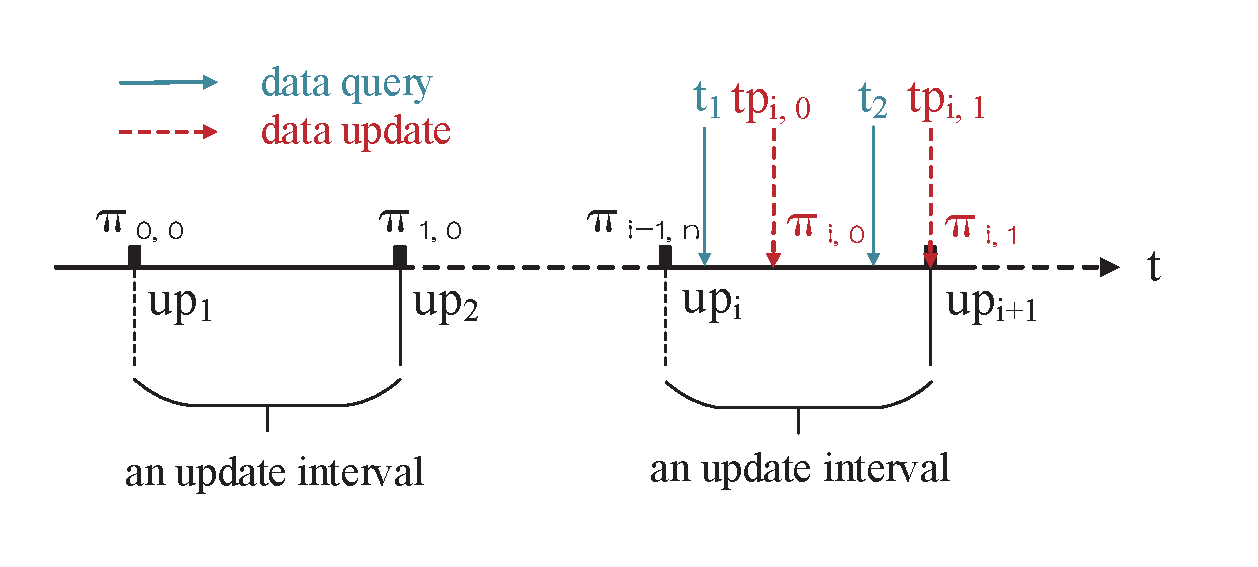
\includegraphics[width=6 in]{fig/timestamp}
  \DeclareGraphicsExtensions.
  \caption{时间戳链的简单示例}
  \label{fig:timestamp}
\end{figure}

如图~\ref{fig:timestamp}所示,横向为时间轴,红色的线表示的是数据持有者的更新时间点,蓝色的线表示的是数据搜索者的查询点。$(up_1,up_2,\cdots,up_i,up_{i+1})$是更新时间点,其中$(up_i,up_{i+1}]$即为一个更新周期,$up_{i+1}$为该更新周期的检测点。
每一个周期中,鉴别符都链式相连,例如图中的$\pi_{i, 0}, \pi_{i, 1}$,但是不同的更新周期内的鉴别符不相连。

让我们考虑如下几种数据搜索用户在不同时刻发起请求的情况:(i) 第一种情况,数据搜索用户在$t_1$时刻发起搜索请求,其中$t_1 < tp_{i, 0}$;(ii) 第二种情况,数据搜索用户在$t_2$时刻发起搜索请求,该请求发生在一次数据更新时刻$tp_{i, 0}$之后,且云服务器发送给用户的鉴别符为$\pi_{i, 0}$;(iii)第三种情况,数据搜索用户仍然在$t_2$时刻发起搜索请求,但是云服务器发送给用户的鉴别符为$\pi_{i-1, n}$。在最后一种情况中,一个数据新鲜性攻击产生,但是它会在检测点$up_{i+1}$被用户发现。用户将在检测点收到鉴别符$\pi_{i, 1}$,通过它用户可以验证用户在查询时刻收到的鉴别符是否正确。

我们仍然采用上述三种情况来描述搜索用户验证鉴别符的过程。在上述第一种情况中,用户将收到鉴别符$\pi_{i, 1}$ 和 $\pi_{i, 0}$,通过它们,用户可以提取出 $\alpha_{i,1}$ 和 $\alpha_{i,0}$。通过$Check$算法,我们可以发现在解密了$\alpha_{i, 0}$后,得到的$\alpha$为$\emptyset$,因此$Check$算法将输出$b=1$ 并且在搜索时刻收到的鉴别符$\pi_{i-1, n}$是正确的。在第二种情况中,$\alpha_{i, 0}$ 同样通过 $\alpha_{i, 1}$ 被解密出,并且 $\alpha_{i, 0}$的时间戳已经早于 $t_2$. 我们可以通过对比发现解密得到的鉴别符$\alpha_{i, 0}$ 与在搜索时刻收到的鉴别符 $\alpha^{t_2}_q$ 相等. 因此 $\alpha^{t_2}_q$ 也被认为是正确的,即 $\pi^{t_2}_q$ 中包含的根哈希是正确的。然而,在最后一种情况中,我们将会发现数据新鲜性攻击,因为解密得到的鉴别符$\pi_{i, 0}$与用户在搜索时刻得到的鉴别符$\pi_{i-1, n}$不相等。

\section{安全性分析}
在本节中,我们将对\multi 方案的安全性进行证明。与\single 方案相同,需要从机密性和可验证性两个角度对\multi 方案进行证明。
在证明开始前,我们需要明确\multi 方案与\single 方案的差别。\multi 方案通过引入鉴别符$\pi$的方式将根哈希和时间戳进行了绑定,搜索用户通过解密鉴别符,得到其中包含的最新根哈希来对数据新鲜性和数据完整性进行验证。除此之外,\multi 方案的其他步骤均与\single 方案相同。因此我们只需证明鉴别符$\pi$的引入仍然可以保证数据的机密性和结果的可验证性。我们有以下的定理:
\begin{theorem}
    如果$(ssk,spk)$是签名公私钥对,$K_3$是对称秘钥,那么\multi 方案就是机密且可验证的。
\end{theorem}

\begin{proof}
    首先证明机密性。由于鉴别符$\pi$通过数据持有者的对称秘钥$K_3$进行了加密,因此敌手只要没有该对称秘钥,即无法获知鉴别符的内容。因此鉴别符的机密性是可以保证的。
    其次证明可验证性。由于鉴别符$\pi$通过数据持有者的签名私钥$ssk$进行了签名,敌手没有该私钥就无法伪造数据持有者的签名。因此也无法生成鉴别符,让搜索用户使用公钥$spk$验证通过。一个由数据搜索用户验证了的、由数据持有者生成的鉴别符,最多只能因为服务器的恶意行为而产生数据新鲜性攻击,而该攻击已经通过$Check$算法解决。因此\multi 算法是可验证的。
\end{proof}

\section{实验结果}
\subsection{实验设置}
为了证明\multi 方案的有效性,我们采用一台处理器为Inter Core i5 2.3GHz,内存为4G的笔记本上进行实验,实验采用单线程执行。
下文中,我们首先对\multi 方案引入的数据持有者端的带宽开销进行了验证,随后对\multi 方案所需的结果验证时间进行了评估。
\subsection{实验结果}
\label{sec:experiments}
\begin{figure}[ht]
  \begin{minipage}[b]{0.49\textwidth}
    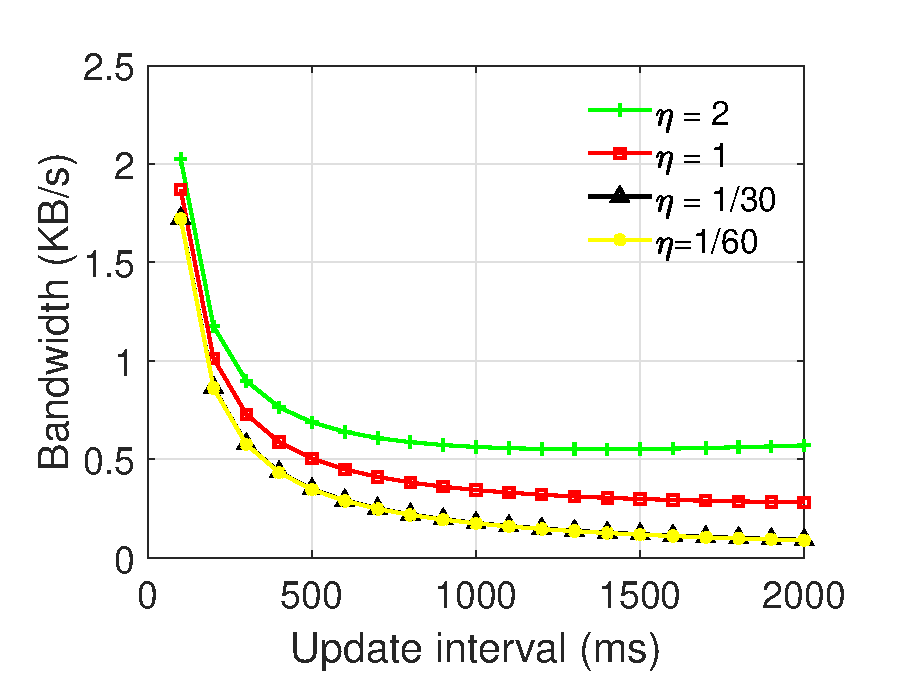
\includegraphics[width= 3 in]{expr/bandwidth}
    \caption{带宽开销}
    \label{fig:bandwidth}
  \end{minipage}
  \begin{minipage}[b]{0.49\textwidth}
    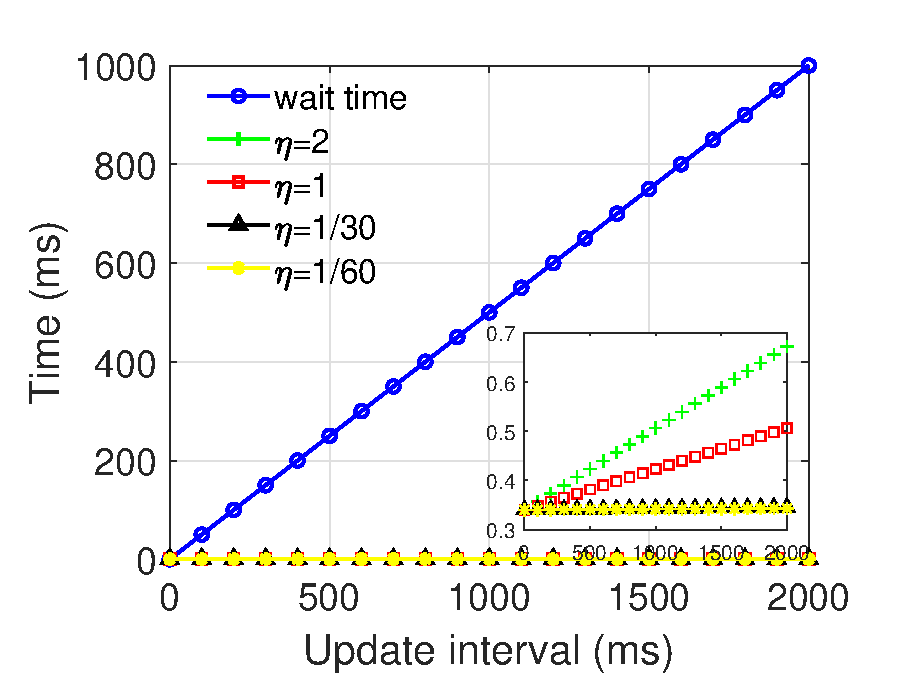
\includegraphics[width= 3 in]{expr/verify-2}
    \caption{总验证时间开销}
    \label{fig:verify-2}
  \end{minipage}
\centering
\end{figure}

图~\ref{fig:bandwidth}和图~\ref{fig:verify-2}评估了\multi 方案的开销,包括数据持有者的通信开销和数据搜索用户的验证开销。图中的$\eta$表示数据持有者的数据更新频率。

首先,我们考虑数据持有者端的通信开销。如图~\ref{fig:bandwidth}所示,我们主要考虑由鉴别符带来的开销。这里,每一个更新周期内的第一个鉴别符大小约为112字节,包括了32字节的验证索引根哈希开销,8字节的时间戳开销,8字节的AES-CBC扩展开销,以及128字节的RSA签名开销。总体来说,鉴别符引起的带宽开销包括以下两个部分:由固定更新点导致的鉴别符更新开销和数据更新导致的鉴别符更新开销。
图~\ref{fig:bandwidth}中的曲线充分体现了这两种更新带来的开销。我们可以发现当更新周期接近0时,鉴别符到来的带宽开销接近每秒2KB,这是由固定更新点导致的鉴别符开销,它是与带宽开销成反比的,即更新周期越小,固定更新点越密集,带宽开销越大。此外,带宽开销又随着更新周期的增长缓慢上升,这是由鉴别符自身长度增长带来的带宽开销增长。因为更新周期越长,一个更新周期内产生的鉴别符数量越大,嵌套生成的鉴别符的长度也就越大。

其次,我们考虑数据搜索用户端的验证开销。这部分开销包括用户等待检测点的时间以及执行$Check$算法和$Generate$算法的时间。由于$Generate$算法的开销几乎可以忽略,即0.1毫秒。因此图~\ref{fig:verify-2}中并未标注该部分开销。
这里, $\eta$表示数据持有者的更新频率,我们假设数据搜索在一个更新周期内发起搜索请求的时刻是均匀分布的,则用户等待检测点的时间也呈均匀分布。即,等待检测点的平均时间为半个更新周期的长短,这将占整个验证时延的大部分。$Check$算法与更新周期成正比,这主要由验证鉴别符的签名和解密鉴别符这两种开销导致,但是它相对等待检测点的时间是可以忽略的。需要特别说明的是,在以上的实验中,我们没有将网络的传输时间考虑在内,因为网络传输时间在不同的环境中差异非常大,并且根据我们的方案,传输时延对方案的影响不会很大。
从图\ref{fig:bandwidth}中我们可以看到,当更新频率在2Hz到1/60Hz不等时,数据搜索用户端的验证开销主要取决于等待检测点所需的时间,即和更新间隔的设置有关。

根据以上的实验结果,\multi 方案引入的带宽开销是可以接受的。总体来说,为了在验证时延和带宽开销之间寻找一个平衡点,我们建议可以将更新周期设置在500毫秒置1500毫秒之间。

\section{本章总结}
本章通过方案定义,方案描述,安全性分析和实验分析等方面对\multi 方案进行了分析与阐述,\multi 方案基于不可信云存储环境,为用户提供了一种数据共享场景下的可验证对称加密搜索解决方案,总体来说,\multi 方案的贡献有以下几点:
\begin{itemize}
  \item 完善性。\multi 方案首次为数据共享场景下的可验证加密搜索提出了解决方案,该方案使得可验证加密搜索方案的功能性更加完善,适用场景更加广泛,普适性得到了进一步提升。
  \item 高效性。通过实验验证,\multi 方案为数据持有者和合法用户带来的通信开销和计算开销都很小,在方案有效的前提下保证了其高效性。
\end{itemize}

\chapter{总结与展望}
\label{cha:conclusion}


%%% 其它部分
\backmatter

%% 本科生要这几个索引,研究生不要。选择性留下。
% 插图索引
%\listoffigures
% 表格索引
%\listoftables
% 公式索引
%\listofequations


%% 参考文献
% 注意:至少需要引用一篇参考文献,否则下面两行可能引起编译错误。
% 如果不需要参考文献,请将下面两行删除或注释掉。
% 数字式引用
\bibliographystyle{thuthesis-numeric}
% 作者-年份式引用
% \bibliographystyle{thuthesis-author-year}
\bibliography{ref/refs}


%% 致谢
% 如果使用声明扫描页,将可选参数指定为扫描后的 PDF 文件名,例如:
% \begin{acknowledgement}[scan-statement.pdf]
\begin{acknowledgement}

  三年的研究生生涯如同白驹过隙,一晃而过。从小学到研究生,将近二十年的求学生涯即将结束,却是越长大越珍惜当学生的机会。衷心感谢导师 李琦 教授,香港城市大学 王聪 教授, 武汉大学 王骞教授对本人的精心指导。他们的言传身教将使我终生受益。

  感谢 宋奇阳 同学,以及实验室全体老师和同学们的热情帮助和支持,帮我节省了不少时间。
  本课题承蒙国家自然科学基金资助,特此致谢。

%在这三年多的科研生活里,我从各位老师和同学那儿学到了很多专业知识和研究技能。在此,我要感谢曾经给予我帮助的老师和同学。
%首先我要衷心感谢我的指导老师刘永进老师。刘老师是一个学识渊博,工作负责的老师,在这三年的科研生活中,不管是在学术指导还是在日常生活上,他都给予了我很多的关怀和帮助。他认真的工作态度和渊博的学术知识都是值得我们敬佩和学习的。
%其次,我要感谢中科院软件所的马翠霞老师。马老师是一个非常勤奋和细心的人。在每天的科研工作里,我都能感受到马老师诲人不倦,孜孜以求的态度。在我刚刚踏入科研工作的时间里,她时常指导我解决在具体工作中遇到问题的一些棘手的问题。
%然后,我要感谢中科院心理所的傅小兰老师,王甦菁博士和颜文靖博士。他们在心理学领域给予了我很多的帮助,让我顺利地完成了我的硕士毕业论文。
%最后,我要感谢与我一起工作生活的实验室伙伴们。在忙碌而充实的科研生活中,有了你们的关心和帮助,我才能在这条路上走得如此顺利。
\end{acknowledgement}


%% 附录
%\begin{appendix}
%\chapter{外文资料原文}
\label{cha:engorg}

\title{The title of the English paper}

\textbf{Abstract:} As one of the most widely used techniques in operations
research, \emph{ mathematical programming} is defined as a means of maximizing a
quantity known as \emph{bjective function}, subject to a set of constraints
represented by equations and inequalities. Some known subtopics of mathematical
programming are linear programming, nonlinear programming, multiobjective
programming, goal programming, dynamic programming, and multilevel
programming$^{[1]}$.

It is impossible to cover in a single chapter every concept of mathematical
programming. This chapter introduces only the basic concepts and techniques of
mathematical programming such that readers gain an understanding of them
throughout the book$^{[2,3]}$.


\section{Single-Objective Programming}
The general form of single-objective programming (SOP) is written
as follows,
\begin{equation}\tag*{(123)} % 如果附录中的公式不想让它出现在公式索引中,那就请
                             % 用 \tag*{xxxx}
\left\{\begin{array}{l}
\max \,\,f(x)\\[0.1 cm]
\mbox{subject to:} \\ [0.1 cm]
\qquad g_j(x)\le 0,\quad j=1,2,\cdots,p
\end{array}\right.
\end{equation}
which maximizes a real-valued function $f$ of
$x=(x_1,x_2,\cdots,x_n)$ subject to a set of constraints.

\newtheorem{mpdef}{Definition}[chapter]
\begin{mpdef}
In SOP, we call $x$ a decision vector, and
$x_1,x_2,\cdots,x_n$ decision variables. The function
$f$ is called the objective function. The set
\begin{equation}\tag*{(456)} % 这里同理,其它不再一一指定。
S=\left\{x\in\Re^n\bigm|g_j(x)\le 0,\,j=1,2,\cdots,p\right\}
\end{equation}
is called the feasible set. An element $x$ in $S$ is called a
feasible solution.
\end{mpdef}

\newtheorem{mpdefop}[mpdef]{Definition}
\begin{mpdefop}
A feasible solution $x^*$ is called the optimal
solution of SOP if and only if
\begin{equation}
f(x^*)\ge f(x)
\end{equation}
for any feasible solution $x$.
\end{mpdefop}

One of the outstanding contributions to mathematical programming was known as
the Kuhn-Tucker conditions\ref{eq:ktc}. In order to introduce them, let us give
some definitions. An inequality constraint $g_j(x)\le 0$ is said to be active at
a point $x^*$ if $g_j(x^*)=0$. A point $x^*$ satisfying $g_j(x^*)\le 0$ is said
to be regular if the gradient vectors $\nabla g_j(x)$ of all active constraints
are linearly independent.

Let $x^*$ be a regular point of the constraints of SOP and assume that all the
functions $f(x)$ and $g_j(x),j=1,2,\cdots,p$ are differentiable. If $x^*$ is a
local optimal solution, then there exist Lagrange multipliers
$\lambda_j,j=1,2,\cdots,p$ such that the following Kuhn-Tucker conditions hold,
\begin{equation}
\label{eq:ktc}
\left\{\begin{array}{l}
    \nabla f(x^*)-\sum\limits_{j=1}^p\lambda_j\nabla g_j(x^*)=0\\[0.3cm]
    \lambda_jg_j(x^*)=0,\quad j=1,2,\cdots,p\\[0.2cm]
    \lambda_j\ge 0,\quad j=1,2,\cdots,p.
\end{array}\right.
\end{equation}
If all the functions $f(x)$ and $g_j(x),j=1,2,\cdots,p$ are convex and
differentiable, and the point $x^*$ satisfies the Kuhn-Tucker conditions
(\ref{eq:ktc}), then it has been proved that the point $x^*$ is a global optimal
solution of SOP.

\subsection{Linear Programming}
\label{sec:lp}

If the functions $f(x),g_j(x),j=1,2,\cdots,p$ are all linear, then SOP is called
a {\em linear programming}.

The feasible set of linear is always convex. A point $x$ is called an extreme
point of convex set $S$ if $x\in S$ and $x$ cannot be expressed as a convex
combination of two points in $S$. It has been shown that the optimal solution to
linear programming corresponds to an extreme point of its feasible set provided
that the feasible set $S$ is bounded. This fact is the basis of the {\em simplex
  algorithm} which was developed by Dantzig as a very efficient method for
solving linear programming.
\begin{table}[ht]
\centering
  \centering
  \caption*{Table~1\hskip1em This is an example for manually numbered table, which
    would not appear in the list of tables}
  \label{tab:badtabular2}
  \begin{tabular}[c]{|m{1.5cm}|c|c|c|c|c|c|}\hline
    \multicolumn{2}{|c|}{Network Topology} & \# of nodes &
    \multicolumn{3}{c|}{\# of clients} & Server \\\hline
    GT-ITM & Waxman Transit-Stub & 600 &
    \multirow{2}{2em}{2\%}&
    \multirow{2}{2em}{10\%}&
    \multirow{2}{2em}{50\%}&
    \multirow{2}{1.2in}{Max. Connectivity}\\\cline{1-3}
    \multicolumn{2}{|c|}{Inet-2.1} & 6000 & & & &\\\hline
    \multirow{2}{1.5cm}{Xue} & Rui  & Ni &\multicolumn{4}{c|}{\multirow{2}*{\thuthesis}}\\\cline{2-3}
    & \multicolumn{2}{c|}{ABCDEF} &\multicolumn{4}{c|}{} \\\hline
\end{tabular}
\end{table}

Roughly speaking, the simplex algorithm examines only the extreme points of the
feasible set, rather than all feasible points. At first, the simplex algorithm
selects an extreme point as the initial point. The successive extreme point is
selected so as to improve the objective function value. The procedure is
repeated until no improvement in objective function value can be made. The last
extreme point is the optimal solution.

\subsection{Nonlinear Programming}

If at least one of the functions $f(x),g_j(x),j=1,2,\cdots,p$ is nonlinear, then
SOP is called a {\em nonlinear programming}.

A large number of classical optimization methods have been developed to treat
special-structural nonlinear programming based on the mathematical theory
concerned with analyzing the structure of problems.
\begin{figure}[h]
  \centering
  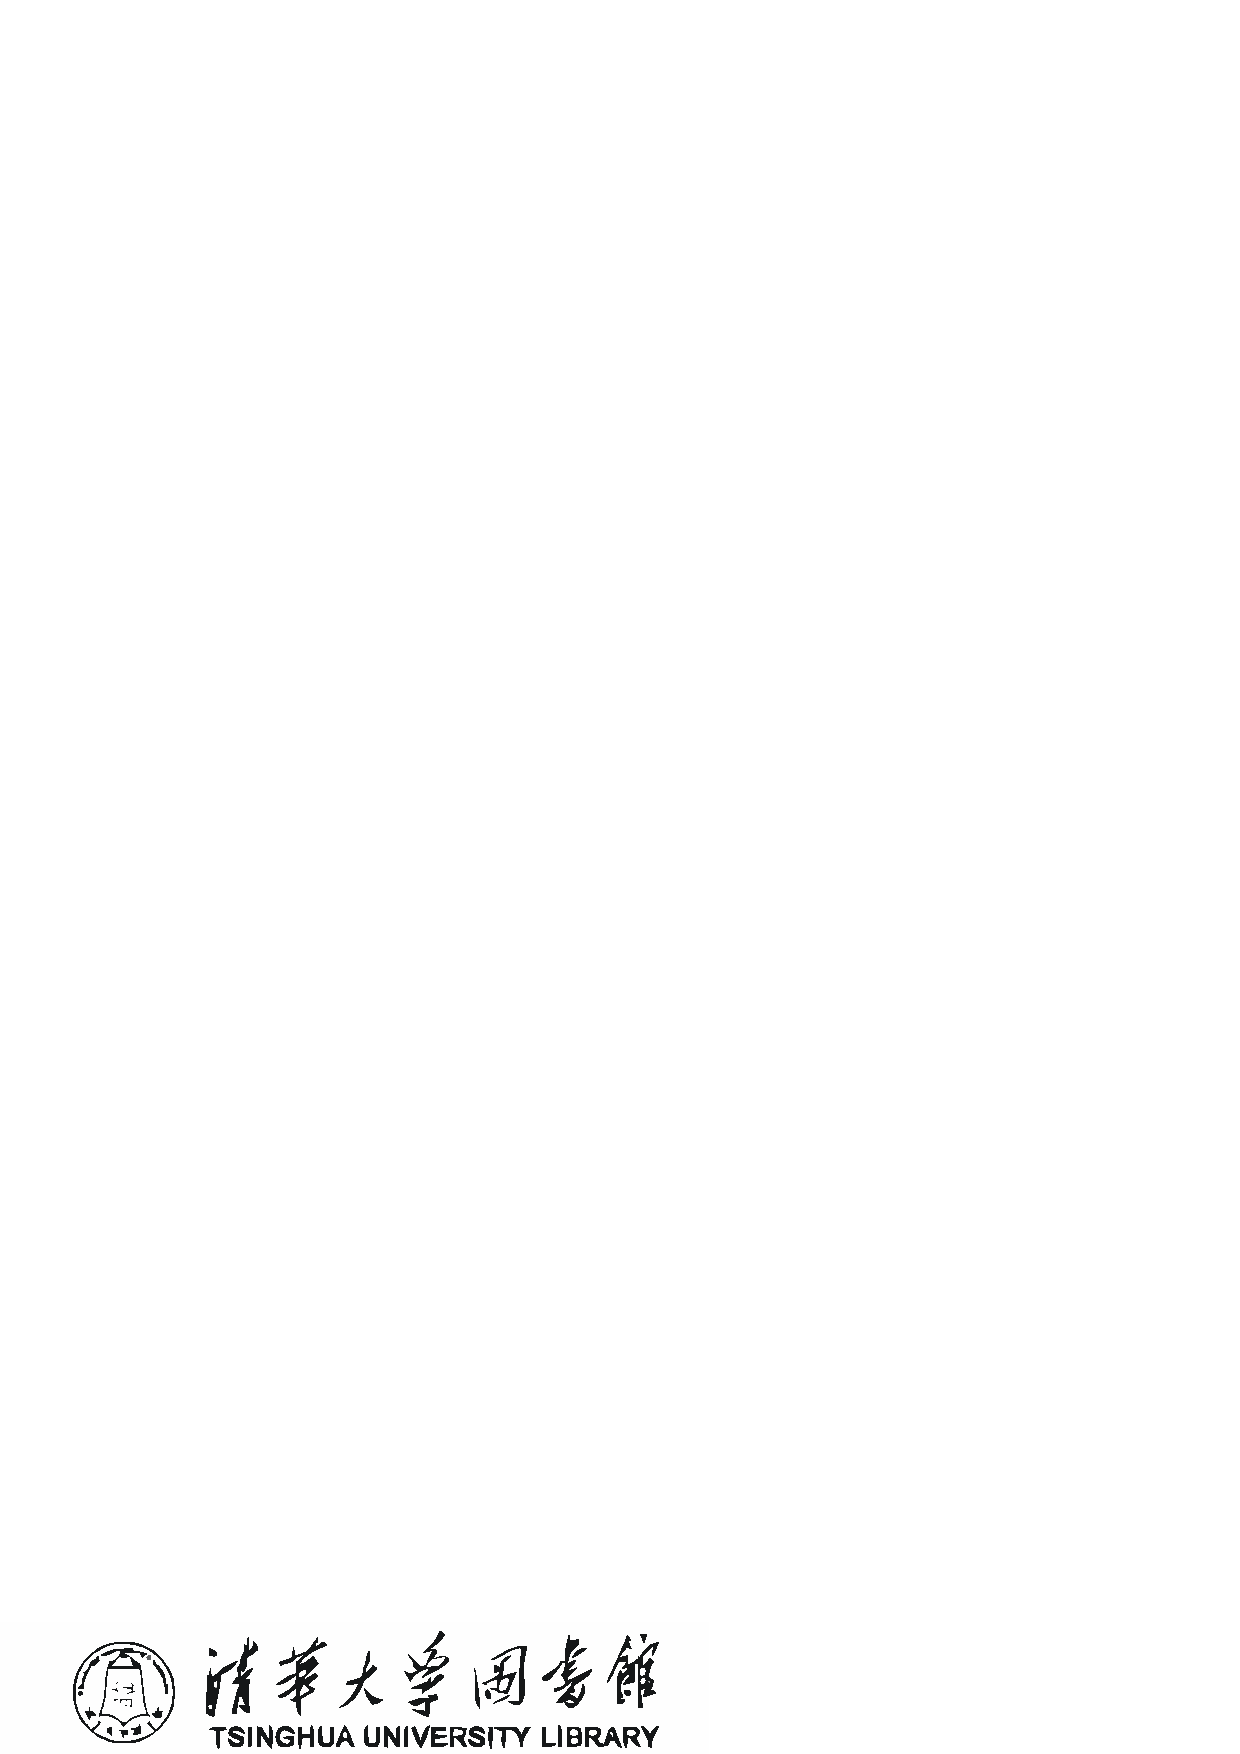
\includegraphics{thu-lib-logo}
  \caption*{Figure~1\quad This is an example for manually numbered figure,
    which would not appear in the list of figures}
  \label{tab:badfigure2}
\end{figure}

Now we consider a nonlinear programming which is confronted solely with
maximizing a real-valued function with domain $\Re^n$.  Whether derivatives are
available or not, the usual strategy is first to select a point in $\Re^n$ which
is thought to be the most likely place where the maximum exists. If there is no
information available on which to base such a selection, a point is chosen at
random. From this first point an attempt is made to construct a sequence of
points, each of which yields an improved objective function value over its
predecessor. The next point to be added to the sequence is chosen by analyzing
the behavior of the function at the previous points. This construction continues
until some termination criterion is met. Methods based upon this strategy are
called {\em ascent methods}, which can be classified as {\em direct methods},
{\em gradient methods}, and {\em Hessian methods} according to the information
about the behavior of objective function $f$. Direct methods require only that
the function can be evaluated at each point. Gradient methods require the
evaluation of first derivatives of $f$. Hessian methods require the evaluation
of second derivatives. In fact, there is no superior method for all
problems. The efficiency of a method is very much dependent upon the objective
function.

\subsection{Integer Programming}

{\em Integer programming} is a special mathematical programming in which all of
the variables are assumed to be only integer values. When there are not only
integer variables but also conventional continuous variables, we call it {\em
  mixed integer programming}. If all the variables are assumed either 0 or 1,
then the problem is termed a {\em zero-one programming}. Although integer
programming can be solved by an {\em exhaustive enumeration} theoretically, it
is impractical to solve realistically sized integer programming problems. The
most successful algorithm so far found to solve integer programming is called
the {\em branch-and-bound enumeration} developed by Balas (1965) and Dakin
(1965). The other technique to integer programming is the {\em cutting plane
  method} developed by Gomory (1959).

\hfill\textit{Uncertain Programming\/}\quad(\textsl{BaoDing Liu, 2006.2})

\section*{References}
\noindent{\itshape NOTE: These references are only for demonstration. They are
  not real citations in the original text.}

\begin{translationbib}
\item Donald E. Knuth. The \TeX book. Addison-Wesley, 1984. ISBN: 0-201-13448-9
\item Paul W. Abrahams, Karl Berry and Kathryn A. Hargreaves. \TeX\ for the
  Impatient. Addison-Wesley, 1990. ISBN: 0-201-51375-7
\item David Salomon. The advanced \TeX book.  New York : Springer, 1995. ISBN:0-387-94556-3
\end{translationbib}

\chapter{外文资料的调研阅读报告或书面翻译}

\title{英文资料的中文标题}

{\heiti 摘要:} 本章为外文资料翻译内容。如果有摘要可以直接写上来,这部分好像没有
明确的规定。

\section{单目标规划}
北冥有鱼,其名为鲲。鲲之大,不知其几千里也。化而为鸟,其名为鹏。鹏之背,不知其几
千里也。怒而飞,其翼若垂天之云。是鸟也,海运则将徙于南冥。南冥者,天池也。
\begin{equation}\tag*{(123)}
 p(y|\mathbf{x}) = \frac{p(\mathbf{x},y)}{p(\mathbf{x})}=
\frac{p(\mathbf{x}|y)p(y)}{p(\mathbf{x})}
\end{equation}

吾生也有涯,而知也无涯。以有涯随无涯,殆已!已而为知者,殆而已矣!为善无近名,为
恶无近刑,缘督以为经,可以保身,可以全生,可以养亲,可以尽年。

\subsection{线性规划}
庖丁为文惠君解牛,手之所触,肩之所倚,足之所履,膝之所倚,砉然响然,奏刀騞然,莫
不中音,合于桑林之舞,乃中经首之会。
\begin{table}[ht]
\centering
  \centering
  \caption*{表~1\hskip1em 这是手动编号但不出现在索引中的一个表格例子}
  \label{tab:badtabular3}
  \begin{tabular}[c]{|m{1.5cm}|c|c|c|c|c|c|}\hline
    \multicolumn{2}{|c|}{Network Topology} & \# of nodes &
    \multicolumn{3}{c|}{\# of clients} & Server \\\hline
    GT-ITM & Waxman Transit-Stub & 600 &
    \multirow{2}{2em}{2\%}&
    \multirow{2}{2em}{10\%}&
    \multirow{2}{2em}{50\%}&
    \multirow{2}{1.2in}{Max. Connectivity}\\\cline{1-3}
    \multicolumn{2}{|c|}{Inet-2.1} & 6000 & & & &\\\hline
    \multirow{2}{1.5cm}{Xue} & Rui  & Ni &\multicolumn{4}{c|}{\multirow{2}*{\thuthesis}}\\\cline{2-3}
    & \multicolumn{2}{c|}{ABCDEF} &\multicolumn{4}{c|}{} \\\hline
\end{tabular}
\end{table}

文惠君曰:“嘻,善哉!技盖至此乎?”庖丁释刀对曰:“臣之所好者道也,进乎技矣。始臣之
解牛之时,所见无非全牛者;三年之后,未尝见全牛也;方今之时,臣以神遇而不以目视,
官知止而神欲行。依乎天理,批大郤,导大窾,因其固然。技经肯綮之未尝,而况大坬乎!
良庖岁更刀,割也;族庖月更刀,折也;今臣之刀十九年矣,所解数千牛矣,而刀刃若新发
于硎。彼节者有间而刀刃者无厚,以无厚入有间,恢恢乎其于游刃必有余地矣。是以十九年
而刀刃若新发于硎。虽然,每至于族,吾见其难为,怵然为戒,视为止,行为迟,动刀甚微,
謋然已解,如土委地。提刀而立,为之而四顾,为之踌躇满志,善刀而藏之。”

文惠君曰:“善哉!吾闻庖丁之言,得养生焉。”


\subsection{非线性规划}
孔子与柳下季为友,柳下季之弟名曰盗跖。盗跖从卒九千人,横行天下,侵暴诸侯。穴室枢
户,驱人牛马,取人妇女。贪得忘亲,不顾父母兄弟,不祭先祖。所过之邑,大国守城,小
国入保,万民苦之。孔子谓柳下季曰:“夫为人父者,必能诏其子;为人兄者,必能教其弟。
若父不能诏其子,兄不能教其弟,则无贵父子兄弟之亲矣。今先生,世之才士也,弟为盗
跖,为天下害,而弗能教也,丘窃为先生羞之。丘请为先生往说之。”
\begin{figure}[h]
  \centering
  
\includegraphics{thu-whole-logo}
  \caption*{图~1\hskip1em 这是手动编号但不出现索引中的图片的例子}
  \label{tab:badfigure3}
\end{figure}

柳下季曰:“先生言为人父者必能诏其子,为人兄者必能教其弟,若子不听父之诏,弟不受
兄之教,虽今先生之辩,将奈之何哉?且跖之为人也,心如涌泉,意如飘风,强足以距敌,
辩足以饰非。顺其心则喜,逆其心则怒,易辱人以言。先生必无往。”

孔子不听,颜回为驭,子贡为右,往见盗跖。

\subsection{整数规划}
盗跖乃方休卒徒大山之阳,脍人肝而餔之。孔子下车而前,见谒者曰:“鲁人孔丘,闻将军
高义,敬再拜谒者。”谒者入通。盗跖闻之大怒,目如明星,发上指冠,曰:“此夫鲁国之
巧伪人孔丘非邪?为我告之:尔作言造语,妄称文、武,冠枝木之冠,带死牛之胁,多辞缪
说,不耕而食,不织而衣,摇唇鼓舌,擅生是非,以迷天下之主,使天下学士不反其本,妄
作孝弟,而侥幸于封侯富贵者也。子之罪大极重,疾走归!不然,我将以子肝益昼餔之膳。”


\chapter{其它附录}
前面两个附录主要是给本科生做例子。其它附录的内容可以放到这里,当然如果你愿意,可
以把这部分也放到独立的文件中,然后将其 \cs{input} 到主文件中。

%\end{appendix}

%% 个人简历
\begin{resume}

  \resumeitem{个人简历}

  xxxx 年 xx 月 xx 日出生于 xx 省 xx 县。

  xxxx 年 9 月考入 xx 大学 xx 系 xx 专业,xxxx 年 7 月本科毕业并获得 xx 学士学位。

  xxxx 年 9 月免试进入 xx 大学 xx 系攻读 xx 学位至今。

  \researchitem{发表的学术论文} % 发表的和录用的合在一起

  % 1. 已经刊载的学术论文(本人是第一作者,或者导师为第一作者本人是第二作者)
  \begin{publications}
    \item Yang Y, Ren T L, Zhang L T, et al. Miniature microphone with silicon-
      based ferroelectric thin films. Integrated Ferroelectrics, 2003,
      52:229-235. (SCI 收录, 检索号:758FZ.)
    \item 杨轶, 张宁欣, 任天令, 等. 硅基铁电微声学器件中薄膜残余应力的研究. 中国机
      械工程, 2005, 16(14):1289-1291. (EI 收录, 检索号:0534931 2907.)
    \item 杨轶, 张宁欣, 任天令, 等. 集成铁电器件中的关键工艺研究. 仪器仪表学报,
      2003, 24(S4):192-193. (EI 源刊.)
  \end{publications}

  % 2. 尚未刊载,但已经接到正式录用函的学术论文(本人为第一作者,或者
  %    导师为第一作者本人是第二作者)。
  \begin{publications}[before=\publicationskip,after=\publicationskip]
    \item Yang Y, Ren T L, Zhu Y P, et al. PMUTs for handwriting recognition. In
      press. (已被 Integrated Ferroelectrics 录用. SCI 源刊.)
  \end{publications}

  % 3. 其他学术论文。可列出除上述两种情况以外的其他学术论文,但必须是
  %    已经刊载或者收到正式录用函的论文。
  \begin{publications}
    \item Wu X M, Yang Y, Cai J, et al. Measurements of ferroelectric MEMS
      microphones. Integrated Ferroelectrics, 2005, 69:417-429. (SCI 收录, 检索号
      :896KM)
    \item 贾泽, 杨轶, 陈兢, 等. 用于压电和电容微麦克风的体硅腐蚀相关研究. 压电与声
      光, 2006, 28(1):117-119. (EI 收录, 检索号:06129773469)
    \item 伍晓明, 杨轶, 张宁欣, 等. 基于MEMS技术的集成铁电硅微麦克风. 中国集成电路,
      2003, 53:59-61.
  \end{publications}

  \researchitem{研究成果} % 有就写,没有就删除
  \begin{achievements}
    \item 任天令, 杨轶, 朱一平, 等. 硅基铁电微声学传感器畴极化区域控制和电极连接的
      方法: 中国, CN1602118A. (中国专利公开号)
    \item Ren T L, Yang Y, Zhu Y P, et al. Piezoelectric micro acoustic sensor
      based on ferroelectric materials: USA, No.11/215, 102. (美国发明专利申请号)
  \end{achievements}

\end{resume}


%% 本科生进行格式审查是需要下面这个表格,答辩可能不需要。选择性留下。
% 综合论文训练记录表
%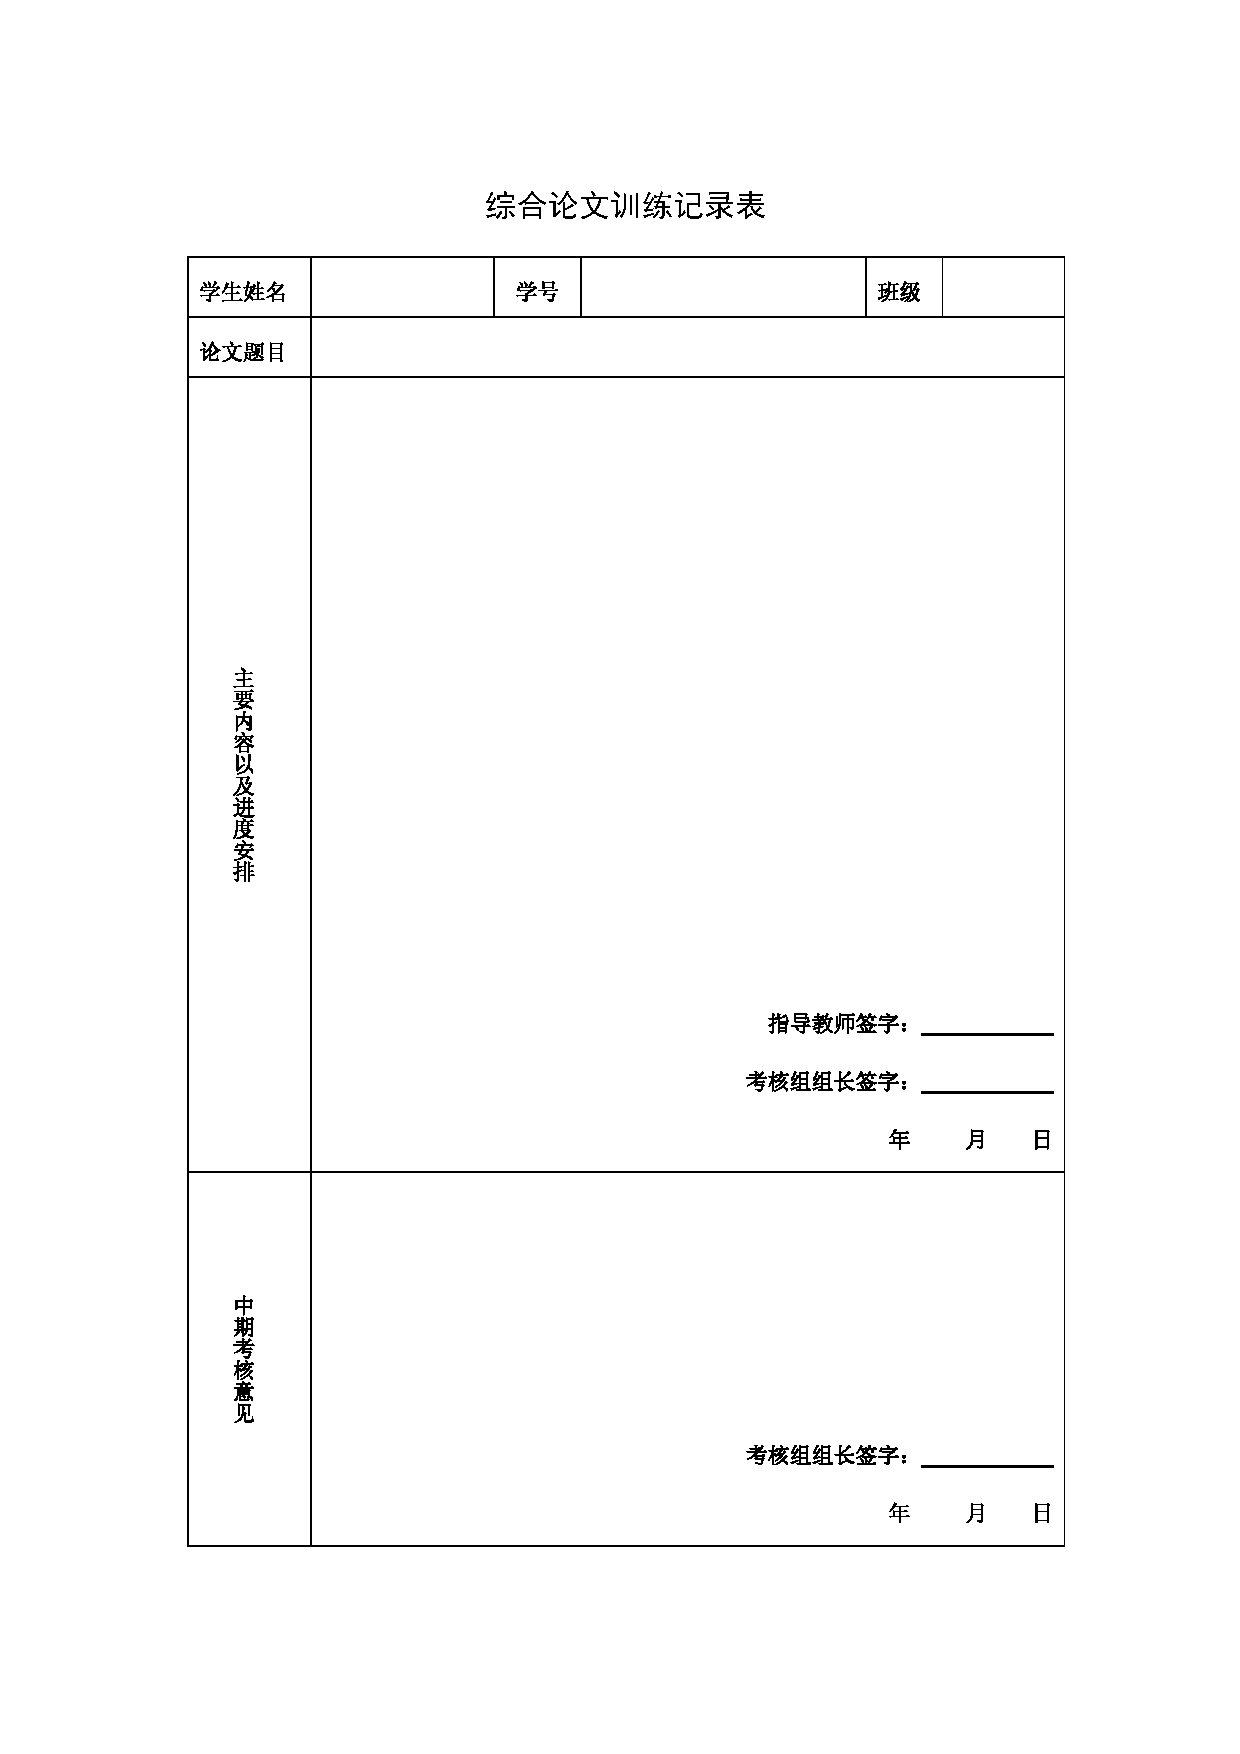
\includepdf[pages=-]{scan-record.pdf}
\end{document}
